\documentclass{scrbook}
\usepackage{amstext}
\usepackage{ulem}
\usepackage[ngerman]{babel}
\usepackage{amssymb}
\usepackage{amsmath}
\usepackage[utf8]{inputenc}
\usepackage{hhline}
\usepackage{multirow}
\usepackage{graphicx}
\usepackage{ mathrsfs }
\usepackage{ gensymb }
\usepackage[colorlinks,pdfpagelabels,pdfstartview = FitH,bookmarksopen = true,bookmarksnumbered = true,linkcolor = black,plainpages = false,hypertexnames = false,citecolor = black] {hyperref}
\begin{document}
\frontmatter
\begin{titlepage}
\title{Mathe für Informatiker II}
\subtitle{Mitschrift der Vorlesung von Christian Bender Sommersemester 17}
\author{Lukas Koschorke}
\date{\today}
\maketitle
\end{titlepage}
\section*{Vorwort}
Hallo zusammen, ich versuche mein Skript immer aktuell zu halten und wenn ich es eh schon abtippe, kann ich es auch noch zusätzlich auf StudyDrive hochladen. Ich kann leider keine Garantie geben, dass es immer den kompletten Stoff aller Vorlesungen beinhaltet, auch wenn ich mein Bestes dafür gebe. Wenn euch Fehler auffallen, haut sie einfach in die Kommentare von StudyDrive.
\tableofcontents
\mainmatter
\chapter{Lineare Gleichungssysteme und der Gaußalgorithmus}
\section{Beispiel (PageRank)}
Ein Nutzer surft auf den vorhandenen Seiten des Internets S\textsubscript{1},...,S\textsubscript{N}. Er beginnt auf irgendeiner Seite und folgt typischerweise einem der Links. Er kann aber auch auf eine beliebige Seite springen.\\
Zur Modellierung sei \(0<d<1\) (Damping-Faktor, typischerweise \(d=0,85\)).
Auf einer Seite angekommen, folgt der Nutzer mit Wahrscheinlichkeit d einem rein zufällig ausgewähltem Link, mit Wahrscheinlichkeit \(1-d\) springt er auf eine rein zufällig gewählte Seite.
(Konvention: Falls die Seite keinen Outlink hat, so wählt man rein zufällig eine Seite aus.)\\
"`Auf lange Sicht"' (d.h. wenn die Anzahl der Surfschritte gegen unenlich strebt), ist die Wahrscheinlichkeit p\textsubscript{i}, sich auf der Seite S\textsubscript{i} zu befinden, beschrieben durch
\begin{equation}\text{\label{1.1}}
p_{i} =\dfrac{1-d}{N} + d \sum_{j=1}^{N}a_{ij} p_{j}, i=1,...,N
\end{equation}
wobei:
\[
a_{ij}=
\left\{
\begin{array}{ll}
\dfrac{1}{c_{j}} & \text{, falls Seite S\textsubscript{j} auf Seite S\textsubscript{i} verlinkt}\\
\\
\dfrac{1}{N} & \text{, falls S\textsubscript{j} keinen Outlink hat}\\
\\
0 & \text{, sonst} 
\end{array}
\right.
\]
und c\textsubscript{j} die Anzahl an Seiten angibt, auf die S\textsubscript{j} verlinkt (siehe dazu das "`Das Kapital der Markovketten"' in der MFI3).\\
p\textsubscript{i} wird \uline{PageRank} der Seite S\textsubscript{i} genannt.\\
\\
\ref{1.1} ist ein System von N linearen Gleichungen zu N Unbekannten.\\
\\
In einem Netz mit 3 Seiten sei die Verlinkung schematisch dargestellt durch:\\
\[S_1\leftrightarrows S_3,S_2\rightarrow S_1, S_3 \rightarrow S_2\]
\\
Hier ist also \(c_3=2, c_1=c_2=1\), d.h. \ref{1.1}  
wird im Spezialfall zu:
\[\begin{array}{lrlrlrclc}
&p_1&-&d p_2 &-&\dfrac{d}{2}p_3&=&\dfrac{1-d}{3}&(I)\\\\
&&&p_2&-&\dfrac{d}{2}p_3&=&\dfrac{1-d}{3}&(II)\\\\
-&d p_1&&&+&p_3&=&\dfrac{1-d}{3}&(III)\\\\
\end{array}
\]
Indem man \((I)\) durch \((\tilde{I}) = (I)+d(II)+\dfrac{1}{d}(III)\)ersetzt, erhält man die äquivalente Form:
\[\begin{array}{lrlrlrclc}
-&d p_1&&&+&p_3&=&\dfrac{1-d}{3}&(III)\\\\
&&&p_2&-&\dfrac{d}{2}p_3&=&\dfrac{1-d}{3}&(II)\\\\
&&&&&(\dfrac{1}{d}-\dfrac{d^2}{2}-\dfrac{d}{2})p_3&=&\dfrac{1-d}{3}(1+\dfrac{1}{d}+d)&(\tilde{I})\\\\
\end{array}
\]
Nun haben wir das System in "`Zeilenstufenform"' und man kann die Lösung direkt ablesen (\( 0<d<1\)):
\[
\begin{array}{lcl}
p_3&=&\dfrac{1-d}{3}\dfrac{d^2+d+1}{1-\dfrac{d^3}{2}-\dfrac{d^2}{2}}\\
\\
p_2&=&\dfrac{1-d}{3}+\dfrac{d}{2}p_3\\
\\
p_1&=&\dfrac{1}{d}(p_3-\dfrac{1-d}{3})\\
\end{array}
\]
Da \(p_3>\dfrac{1-d}{3}\) folgt \(p_1>0\) und \(p_2>0\).\\
Da ferner \(p_1+p_2+p_3=1\) (Nachrechnen), kann der PageRank tatsächlich als Wahrscheinlichkeit interpretiert werden.\\
Für \(d=0,85\) ist:\\
\(
p_1 \approx 0,397\\
p_2 \approx 0,215\\
p_3 \approx 0,388\\
\)
Betrachten wir den "`Grenzfall"' \(d=1\), in dem nur Links zum Surfen verwendet werden, dann:
\[
\begin{array}{lrlrlrclc}
&p_1&-&p_2 &-&\dfrac{1}{2}p_3&=&0&(I)\\\\
&&&p_2&-&\dfrac{1}{2}p_3&=&0&(II)\\\\
-&p_1&&&+&p_3&=&0&(III)\\\\
\end{array}
\]
und wie zuvor:
\[
\begin{array}{lrlrlrclc}
-&p_1&&&+&p_3&=&0&(III)\\\\
&&&p_2&-&\dfrac{1}{2}p_3&=&0&(II)\\\\
&&&&&0&=&0&(\tilde{I})\\\\
\end{array}
\]
Hier lösen alle \(p_1, p_2, p_3\) der Form
\[p_1=p_3, p_2 = \dfrac{1}{2}p_3,\text{ }p_3\in\mathbb{R}\]
das System \ref{1.1}. Fordert man zusätzlich die Wahrscheinlichkeitsbedingung \(p_1+p_2+p_3=1\), so ist die eindeutige Lösung:
\[p_3=p_1 = 0,4,\text{ } p_2=0,2\]
\\
\textbf{\uwave{Zur Bedeutung des Damping-Faktor:}}
\begin{description}
\item[a)] Die Wahl \(0\leq d<1\) sichert, dass \ref{1.1} genau eine Lösung hat und, dass diese Lösung positive Einträge hat.\\
Dies werden wir im Zusammenhang mit "`Eigenwertproblemen"' besser verstehen.\\
\item[b)] Im realistischen Problem ist N sehr groß (\(N>20Mio.\)). Dann müssen nummerische Verfahren zur Approximation des PageRank herangezogen werden. Wir werden sehen, dass die Wahl von $d$ eine wichtige Rolle bei der Konvergenzgeschwindigkeit derartiger Verfahren spielt.\\
\end{description}
\textbf{\uwave{Problem:}}\\
\\
Gegeben sei ein System von \(m\in\mathbb{N}\) Gleichungen mit \(n\in\mathbb{N}\) Unbekannten:\\
\[
\left.
\begin{array}{ccccccc}
a_{11}x_1 & +  &\cdots & + & a_{1n}x_n & = & b_1\\
\vdots & & \ddots & & \vdots & & \vdots\\
a_{m1}x_1 & + & \cdots & + & a_{mn}x_n & = & b_m
\end{array}
\right\}
(L)
\]
\\
Hierbei seien die Koeffizienten \(a_{ij} \in \mathbb{R}\) (mit doppelter Indexschreibweise) für \(i=1,...,m,\) \(j=1,...,n\), sowie die rechte Seite \(b_i \in \mathbb{R}, i=1,...,m\), gegeben.\\
Gesucht sind alle n-Tupel (\(x_1,...,x_n\)) von reellen Zahlen, die das System (L) lösen.\\
Zur übersichtlichen Notation schreibt man die Koeffizienten als Rechteckschema, das \(m\times n\)-Matrix genannt wird\\
\[
A:=(a_{ij})_{i=1,...,m,j=1,...,n}:=
\left(
\begin{array}{ccc}
a_{11}&\cdots&a_{1n}\\
\vdots&\ddots&\vdots\\
a_{m1}&\cdots&a_{mn}
 \end{array}
 \right)
\]
und die \(b_{i}'s\) und \(x_j's\) als \textbf{Spaltenvektor}
\[
x:=\left(\begin{array}{c}
x_1\\
\vdots\\
x_n
\end{array}\right), b:= \left(
\begin{array}{c}
b_1\\
\vdots\\
b_m
\end{array}\right)
\]
Definiert man nun ein Produkt zwischen \(m\times n\)-Matrix und Spaltenvektor der Höhe n, das einen Spaltenvektor der Höhe m ergibt, durch:
\[
Ax := \left(\begin{array}{c}
\sum^n_{j=1}a_{1j}x_1\\
\vdots\\
\sum^n_{j=1}a_{mj}x_j
\end{array}\right)
\]
dann kann (L) umgeschrieben werden in die Form
\[Ax=b \text{ (L'})\]
als Gleichung von Spaltenvektoren der Höhe m.\\
Wir bezeichnen die Menge aller Spaltenvektoren der Höhe m mit reellen Einträgen als \(\mathbb{R}^n\) und die Menge aller \(m \times n\)-Matrizen mit reellen Einträgen als \(\mathbb{R}^{m \times n}\).Dann ist die Lösungsmenge von (L) gegeben durch:
\[\text{Lös}(A,b):=\{x \in \mathbb{R}^n| Ax=b\}\]
\section{Definition Zeilenstufenform}
Wir sagen, eine \(m \times n\)-Matrix\(A=(a_{ij})_{i=1,...,m,j=1,...,n}\) hat \textbf{Zeilenstufenform}, falls:
\begin{description}
\item[1.] Es gibt ein \(0\leq r\leq m\), sodass in den Zeilen mit Index 1 bis r nicht alle Einträge gleich 0 sind und in der Zeile(r+1) bis m alle Einträge gleich 0 sind\\
und
\item[2.] es gelte\[j_1<...<j_r\] wobei für jedes \(1\leq i \leq r\)\[j_i = min\{j|a_{ij} \neq 0\}\] der niedrigste Spaltenindex angibt, in dem in der i-ten Zeile ein von 0 verschiedener Eintrag steht.\\
Die Zahl $r$ wird \textbf{Zeilenrang} von $A$ genannt.\\
Die Einträge \(a_{i,j_i},i=1,...,r\), werden \textbf{Pivots} genannt.\\
Offenbar gilt: \(r\leq min\{m,n\}\)
\[
A=\left(\begin{array}{cccc}
(*)&&&\\
\hhline{-~~~}
\multicolumn{1}{c|}{0}&(*)&&\\
\hhline{~-~~}
0&0&\ddots&\\
\hhline{~~~~}
0&0&\multicolumn{1}{c|}{0}&(*)\\
\end{array}\right)
\]
Matrix in Zeilenstufenform: Die mit \((*)\) gekennzeichneten Einträge sind die von 0 verschiedenen Pivots, die Einträge unterhalb der "`Stufenlinie"' sind gleich 0, die übrigen Einträge sind beliebig.\\
Im Beispiel 1.1 hat die Koeffizientenmatrix zum System \((III),(II),(\tilde{I})\) Zeilenstufenform, nämlich:\\
\[\left(\begin{array}{ccc}
-d&0&1\\
0&1&-\dfrac{d}{2}\\
0&0&(\dfrac{1}{2}-\dfrac{d^2}{2}-\dfrac{d}{2})
\end{array}\right)\]
\end{description}
\subsubsection*{Fall 1:} Löse \(Ax=b\), wobei A Zeilenstufenform hat.\\
\begin{description}
\item[a)] Durch Umordnung der Spalten und damit Umnummerierung der Unbekannten, kann man stets voraussetzen, dass die Pivots in den ersten r Spalten stehen, d.h \(j_i=i\) für \(1\leq i \leq r\).\\
\uwave{Beispiel:}\\
\[\underbrace{\left(
\begin{array}{cccccc}
0&2&0&4&0&5\\
0&0&1&3&1&0\\
0&0&0&0&3&0\\
0&0&0&0&0&0\\
\end{array}\right)}_{j_1=2,j_2=3,j_3=5}
\rightsquigarrow
\left(\begin{array}{cccccc}
2&0&0&5&0&4\\
0&1&1&0&0&3\\
0&0&3&0&0&0\\
0&0&0&0&0&0\\
\end{array}\right)
\]
\item[b)] Wir betrachten die \textbf{erweiterte Koeffizientenmatrix} zu \(Ax=b\) (A beliebige \(m \times n\)-Matrix).
\[(A,b)=\left(\begin{array}{cccc}
a_{11} &\cdots&a_{1n}&b_1\\
\vdots&\ddots&\vdots&\vdots\\
a_{m1} &\cdots&a_{mn}&b_m\\
\end{array}\right),
\]
bei der die rechte Seite $b$ als (n+1)-te Spalte an die Koeffizientenmatrix angehängt wird. Ist A in Zeilenstufenform mit Pivots in den ersten $r$ Spalten, so
\[(A,b) =
\left(\begin{array}{cccccc}
a_{11}&&&&&b_1\\
\hhline{-~~~~~}
&\multicolumn{1}{|c}{\ddots}&&&&\vdots\\
&&\multicolumn{1}{|c}{a_{rr}}&&&b_r\\
\hhline{~~----}
&&&&&b_{r+1}\\
&&&&&\vdots\\
&&&&&b_m
\end{array}\right)
\]
\end{description}
\section{Algorithmus (Rückwärtseinsetzen)}
\begin{description}
\item[Input:]
\(m \times n\)-Matrix A in Zeilenstufenform mit Zeilenrang $r$ (\(0 \leq r \leq m\)) und Pivots in den ersten $r$ Spalten, \(b \in \mathbb{R}^m\).
\item[Output:]
"`es existiert keine Lösung"' oder eine bijektive Abbildung:
\[
\Phi_{A,b}:\mathbb{R}^{n-r} \rightarrow \text{Lös}(A,b)
\]
\begin{description}
\item[1.] Falls \(b_i \neq 0\) für ein \(i = r+1,...,m\), so gebe "`keine Lösung"' als Output aus.
\item[2.1] Andernfalls setze in Abhängigkeit von \(\lambda =
\left( \begin{array}{c}
\lambda_1\\
\vdots\\
\lambda_{n-r}
\end{array}\right)
\)
\[
x_{r+1}(\lambda):= \lambda_1,\ ...,\ x_n(\lambda):=\lambda_{n-r}
\]
und für \(i=r,...,1\) rekursiv
\[
x_i:=\dfrac{1}{a_{ij}}(b_i-\sum_{j=i+1}^n a_{ij} x_j(\lambda))
\]
\item[2.2] Gebe \(\Phi_{A,b}:\mathbb{R}^{n-r}\rightarrow \text{Lös}(A,b),\lambda\mapsto x(\lambda):=\left(\begin{array}{c}
x_1(\lambda)\\
\vdots\\
x_n(\lambda)
\end{array}\right)
\) aus.
\end{description}
\end{description}
\subsubsection*{Bemerkung:}
Ist \(r=n\), so ist \(\mathbb{R}^{n-r}=\mathbb{R}^0:=\{0\}\) eineindeutig und das Rückwärtseinsetzen liefert genau eine Lösung für \(Ax=b\) .
\subsubsection*{Beweis der Korrektheit des Algorithmus:}
Ist \(b_i \neq 0\) für ein \(i=r+1,...,m\), so lautet die $i$-te Gleichung\[0*x_1+...+0*x_n = b_i \neq 0\]
und kann also für kein \(x \in \mathbb{R}^n\) erfüllt sein. Andernfalls sind die Gleichungen $r+1$ bis $m$ immer erfüllt $(0=0)$.\\
Für \(i=1,...,r\) lautet die i-te Gleichung
\[a_{ii}x_i+a_{i,i+1}x_{i+1}+...+a_{in}x_n=b_i\]
und ist wegen \(a_{ii} \neq 0\) äquivalent zu:
\[
x_i=\dfrac{1}{a_{ii}}(b_i-\sum_{j=i+1}^n a_{ij}x_j)
\]
Also: \(x(\lambda) \in  \text{Lös}(A,b)\) für alle \(\lambda \in \mathbb{R}^{n-r}\)\\
Zur Bijektivität:\\
Injektiv ist klar, da \(x(\lambda) = \left(
\begin{array}{c}
x_1(\lambda)\\
\vdots\\
x_r(\lambda)\\
\lambda_{1}\\
\vdots\\
\lambda_{n-r}
\end{array}\right) \)\\
und also \(x(\lambda) \neq x(\tilde{\lambda})\) für \(\lambda \neq \tilde{\lambda}\).\\
Surjektiv: Sei \(x=\left(\begin{array}{c}
x_1\\
\vdots\\
x_n
\end{array}\right)\) \(\in\) Lös\((A,b)\) . Setze \(\lambda=\left(\begin{array}{c}
x_{i+1}\\
\vdots\\
x_n
\end{array}\right)\).
Dann:
\[
x_{r+i}(\lambda) = \lambda_i = x_{r+i}\ \forall i=1,...,n-r
\]
Für \(i = r,...,1\) folgt induktiv (Induktionsannahme: \(x_j(\lambda)=x_j \ \forall j \geq i+1\)):
\[
x_1(\lambda)=\dfrac{1}{a_{ii}}(b_i-\sum^n_{j=i+1}a_{ij}x_j(\lambda))
=\dfrac{1}{a_{ij}}(b_i-\sum^n_{j=i+1}a_{ij}x_j)=x_i\square\]
\subsubsection*{Fall 2:}
Löse \(Ax=b\), wobei A in allgemeiner Form.\\
\uwave{Strategie:} Finde ein äquivalentes System \(\tilde{A}x=\tilde{b}\) (also mit Lös(\(A,b\))\(= \text{Lös(}\tilde{A},\tilde{b}\text{)}\)), wobei \(\tilde{A}\) Zeilenstufenform hat.\\
Dazu: Unter \textbf{elementaren Zeilenumformungen} einer Matrix verstehen wir (vorläufig):
\begin{description}
\item[1)] Das Vertauschen von zwei Zeilen
\item[2)] Die Addition des \(\lambda\)-fachen der i-ten Zeile zur j-ten Zeile(\(i\neq j, \lambda\in\mathbb{R}\backslash\{0\}\))
\end{description}
\section{Satz}
Sei (A,b) die erweiterte Koeffizientenmatrix zu \(Ax=b\) und (\(\tilde{A},\tilde{b}\)) gehe aus (A,b) durch endlich viele Zeilenumformungen hervor. Dann:
\[
\text{Lös}(A,b)=\text{Lös}(\tilde{A},\tilde{b})
\]
\subsection*{Beweis:}
Es reicht zu zeigen, dass sich die Lösungsmenge bei einer elementaren Zeilenumformung nicht ändert.
\begin{description}
\item[Typ1:]
Da alle Gleichungen in (L) simultan erfüllt sein müssen, ist die Reihenfolge der Gleichungen egal.
\item[Typ2:]
Da nur die Zahlen i und j betroffen sind, reicht es zu zeigen, dass die Systeme
\[
\left.
\begin{array}{rcccrcc}
a_{i1}x_1&+&\cdots &+ &a_{in} x_n &=&b_i\\
a_{j1}x_1&+&\cdots &+ &a_{jn} x_n &=&b_j\\
\end{array}
\right\} (*)
\]
und
\[
\left.
\begin{array}{rcccrcc}
a_{i1}x_1&+&\cdots &+ &a_{in} x_n &=&b_i\\
(a_{j1}+\lambda a_{i1})x_1&+&\cdots &+ & (a_{jn} + \lambda a_{in}) x_n &=&b_j + \lambda b_i\\
\end{array}
\right\} (**)
\]
Löst \(x= \left(\begin{array}{c}
x_1\\
\vdots\\
x_n
\end{array}\right)
\in \mathbb{R}^n
\) das System \((*)\), so auch die erste Gleichung in \((**)\) und durch Addition des \(\lambda\)-fachen der ersten Gleichung in \((*)\) zur zweiten auch die zweite Gleichung in \((**)\).\\
Umgekehrt schließt man analog durch Subtraktion des \(\lambda\)-fachen der 1.Gleichung in \((**)\) von der zweiten. \(\square\)
\end{description}
\section{Satz}
Jede \(m\times n\)-Matrix kann durch endlich viele elementare Zeilenumformungen in Zeilenstufenform überführt werden.\\
Zum Beweis geben wir einen Algorithmus an, der das Geforderte leistet:\\
\section{Algorithmus}
\begin{description}
\item[Input:] \(m\times n\)-Matrix A
\item[Output:]\(m\times n\)-Matrix in Zeilenstufenform\\
\end{description}
\begin{description}
\item[1.] setze \(A_1 = A \), \(p_1=m, q_1 = n\)
\item[2.] Wende so lange die Funktion "`Zeilenstufenschritt"' an, d.h. setzte\\
\(
(A_k,p_k,q_k):= \text{Zeilenstufenschritt} (A_{k-1},p_{k-1},q_{k-1}) \text{ bis min}(p_k,q_k)=0
\)
\item[3.] Nenne den Abbruchindex \(k_0\) und gebe \(A_{k_0}\) aus.\\
\end{description}
Hierbei ist:\\
\\
\textbf{Zeilenstufenschritt}
\[(\mathbb{R}^{m\times n} \times \{0,\cdots ,m\}\times \{0,\cdots ,n\}\rightarrow \mathbb{R}^{m\times n} \times \{0,\cdots ,m\}\times \{0,\cdots ,n\})
\]
Wie folgt definiert:\\
\\
Zeilenstufenschritt(\(A,p,q\)) := (\(\tilde{A},\tilde{p},\tilde{q}\)), wobei:
\begin{description}
\item[1.] Sei \(B= (b_{ij})_{i=1,\cdots ,p,j=1,\cdots ,q} \text{ mit }  b_{ij}:= a_{m-p+i,n-q+j}\)\\
Veranschaulichung:
\[
A=
\left(
\begin{array}{ccccc}
a_{11}&\cdots&a_{1,n-p}&\cdots &a_{1n}\\
\vdots&\ddots&\vdots&\ddots&\vdots\\
a_{m-q,1}&\cdots &a_{m-q,n-p} & \cdots & a_{m-q,n}\\
\hhline{~~~--}
\vdots & \ddots & \vdots &\multicolumn{2}{|c|}{B}\\ 
a_{m1} & \cdots & a_{m,n-p} & \multicolumn{2}{|c|}{} \\
\end{array}
\right)
\]
\item[2.] Ist \(b_{ij} = 0\) für alle \(i=1,\cdots ,p\) und \(j=1,\cdots ,q\), setze \(\tilde{p} = \tilde{q} = 0 \text{ und } \tilde{A} = A\)
\item[3.1] Andernfalls seien: \(j_1 = min\{j\ |\ b_{ij} \neq 0 \text{ für ein }i =1,\cdots ,p\}\)
(die Spalte von B mit minimalem Index, in der ein von 0 verschiedener Eintrag ist.)\\
und \(i_1=min\{i\ |\ b_{ij} \neq 0\}\)
(die Zeile mit minimalem Index, in der \(j_1\)-ten Spalte ein von 0 verschiedener Eintrag steht.)
\item[3.2] Setze \(\tilde{B} = (\tilde{b}_{ij})_{i=1,\cdots , p ,j=1,\cdots ,q}\),
wobei \(\tilde{b}_{1j} := b_{i_1,j}\ \forall j=1,\cdots ,q\)
und für \(i=2,\cdots,p\) und \(j=1,\cdots, q\):
\[
\tilde{b}_{ij} = 
\left\{
\begin{array}{cccccc}
-\dfrac{b_{ij_1}}{\tilde{b}_{1j_1}}&\tilde{b}_{1j}&+&b_{ij}&i\neq i_1\\
-\dfrac{b_{1j_1}}{\tilde{b}_{1,j_1}}&\tilde{b}_{1j}&+&b_{1j}&i= i_1\\
\end{array}
\right.
\]
(Hier wird erst die \(i_1\)-te mit der ersten Zeile vertauscht und dann ein geeignetes Vielfaches der neuen ersten Zeile zu den anderen Zeilen addiert. \(\tilde{B}\) geht also durch elementare Zeilenumformungen aus B hervor.)
\item[3.3] Setze \(\tilde{p} = p-1, \tilde{q = q-j_1}\)
\[
\tilde{A}=
\left(
\begin{array}{ccccc}
a_{11}&\cdots&a_{1,n-p}&\cdots &a_{1n}\\
\vdots&\ddots&\vdots&\ddots&\vdots\\
a_{m-q,1}&\cdots &a_{m-q,n-p} & \cdots & a_{m-q,n}\\
\hhline{~~~--}
\vdots & \ddots & \vdots &\multicolumn{2}{|c|}{\tilde{B}}\\ 
a_{m1} & \cdots & a_{m,n-p} & \multicolumn{2}{|c|}{} \\
\end{array}
\right)
\]
\end{description}
\textbf{Beachte}, die Matrix \(\tilde{B}\) hat die Form\\
\[
\tilde{B}=
\left(
\begin{array}{ccccccc}
0&\cdots&0&b_{i_1,j_1}&*&\cdots&*\\
\vdots&\ddots&\vdots&0&\vdots&\ddots&\vdots\\
\vdots&\ddots&\vdots&\vdots&\vdots&\ddots&\vdots\\
0&\cdots&0&0&*&\cdots&*\\
\end{array}
\right)*:\text{belibige Einträge, }b_{i_1,j_1} \neq 0
\]
\section{Beispiel}
\[
A=
\left(
\begin{array}{ccccc}
0&0&1&2&9\\
0&3&4&5&9\\
0&6&7&8&9\\
0&9&9&9&9
\end{array}
\right)
\rightsquigarrow
\left(
\begin{array}{ccccc}
0&3&4&5&9\\
0&0&1&2&9\\
0&6&7&8&9\\
0&9&9&9&9
\end{array}
\right)
\rightsquigarrow
\left(
\begin{array}{rrrrr}
0&\multicolumn{1}{|c}{3}&4&5&9\\
\hhline{~-~~~}
0&0&1&2&9\\
0&0&-1&-2&-9\\
0&0&-3&-6&-18
\end{array}
\right)=A_2
\]
\[
\rightsquigarrow
\left(
\begin{array}{rrrrr}
0&\multicolumn{1}{|c}{3}&4&5&9\\
\hhline{~-}
0&0&\multicolumn{1}{|c}{1}&2&9\\
\hhline{~~-}
0&0&0&0&0\\
0&0&0&0&9
\end{array}
\right)=A_3
\rightsquigarrow
\left(
\begin{array}{rrrrr}
0&\multicolumn{1}{|c}{3}&4&5&9\\
\hhline{~-}
0&0&\multicolumn{1}{|c}{1}&2&9\\
\hhline{~~--}
0&0&0&0&\multicolumn{1}{|c}{9}\\
\hhline{~~~~-}
0&0&0&0&0
\end{array}
\right)=A_4
\]
\\
\textbf{Wir zeigen:} Algorithmus 1.6 führt jede \(m \times n\)-Matrix A mit endlich vielen elementaren Zeilenumformungen in Zeilenstufenform über.\\\\
\textbf{Beweis:} Da \(min(p_k,q_k)<min(p_{k-1},q_{k-1})\), bricht der Algorithmus nach endlich vielen Schritten ab. Ist \(A_1 = A\) die Nullmatrix, so ist A bereits in Zeilenstufenform und der Algorithmus liefert A als Output. Andernfalls entsteht \(A_2\) aus \(A_1\) durch endlich viele elementare Zeilenumformungen und hat die Form
\[
A_2=
\left(
\begin{array}{ccccccc}
0&\cdots&0&(*)&*&\cdots&*\\
\hhline{~~~~---}
\vdots&\ddots&\vdots&0&\multicolumn{3}{|c|}{}\\
\vdots&\ddots&\vdots&\vdots&\multicolumn{3}{|c|}{B_2}\\
0&\cdots&0&0&\multicolumn{3}{|c|}{}\\
\hhline{~~~~---}
\end{array}
\right)
\]
Der Eintrag \((*) \neq 0\) steht in der \(m-p_2 =1\)-ten Zeile und \(n-q_2\)-ten Spalte. Also ist \(B_2\) eine \(p_2\times q_2\)-Matrix.\\
Ist \(B_2\) de Nullmatrix, so ist \(A_2\) in Zeilenstufenform und der Algorithmus gibt \(A_2\) aus. Andernfalls wird \(B_2\) im nächsten Schritt mit endlich vielen Elementaren Zeilenumformungen auf die Form (1.1) gebracht. Dehnt man diese Umformungen auf die Zeilen 2 bis m von \(A_2\) aus, ändern sich die ersten \(n-q_2\) Spalten von \(A_2\) nicht, da dort nur Nullen stehen.\\
\(A_2\) wird also in diesem Schritt mit endlich vielen elementaren Zeilenumformungen auf die Form
\[
A_3=
\left(
\begin{array}{ccccccccccc}
0&\cdots&0&(*)&*&\cdots&\cdots&\cdots&\cdots&\cdots&*\\
\vdots&\ddots&\vdots&\vdots&0&\cdots&0&(*)&*&\cdots&*\\
\hhline{~~~~~~~~---}
\vdots&\ddots&\vdots&\vdots&\vdots&\cdots&\vdots&0&\multicolumn{3}{|c|}{}\\
\vdots&\ddots&\vdots&\vdots&\vdots&\cdots&\vdots&\vdots&\multicolumn{3}{|c|}{B_3}\\
0&\cdots&0&0&0&\cdots&0&0&\multicolumn{3}{|c|}{}\\
\hhline{~~~~~~~~---}
\end{array}
\right)
\]
gebracht. Induktiv überzeugt man sich leicht, dass der Algorithmus das Geforderte leistet. \(\square \)\\
\\
Diese Überlegungen führen zu:
\section{Algorithmus (Gaußsche Eliminationsverfahren zur Lösung von \(Ax=b\))}
\begin{description}
\item[Input:]
\(m\times n\)-Matrix A, \(b \in \mathbb{R}^m\)\\
\item[Output:]
"`es ex. keine Lösung"' oder (\(0\leq r \leq n\) und eine Bijektion \(\Phi_{A,b}:\mathbb{R}^{n-r}\rightarrow \text{Lös}(A,b)\))\\
\begin{description}
\item[1.]
Bringe die erweiterte Koeffizientenmatrix \((A,b)\) in Zeilenstufenform \((\tilde{A},\tilde{b})\) mit Algorithmus 1.6
\item[2.]
Bestimme den Zeilenrang $r$ von \(\tilde{A}\) ($m$ minus die Anzahl der Nullstellen von \(\tilde{A}\))
\item[3.]
Tausche die Spalten von \(\tilde{A}\)(falls nötig) so, dass die Pivots in den ersten $r$ Spalten stehen. (Wir bezeichnen die entstehende Matrix weiterhin mit \(\tilde{A}\))
\item[4.]
Verwende Algorithmus 1.3 mit Input \(\tilde{A},\tilde{b},r\) und setzen im Existenzfall \(\Phi_{(A,b)}:=\Phi_{(\tilde{A},\tilde{b})}\) (wobei ggf. die Umnummerierung der Unbekannten aus Schritt 3 zu beachten ist).\\
Die Korrektheit des Algorithmus folgt aus Satz 1.4.
\end{description}
\end{description}
\section{Folgerung}
Die Lös\((A,b)\) für \(Ax=b\) ist entweder leer oder einelementig oder überabzählbar unendlich.
\section{Beispiel (Rundungsfehler im Gauß-Algorithmus)}
Zu lösen ist:
\[
\left(
\begin{array}{cc}
10^{-4}&1\\
1&1
\end{array}
\right)
\left(
\begin{array}{c}
x_1\\
x_2
\end{array}
\right)=
\left(
\begin{array}{c}
1\\
2
\end{array}
\right)
\]
Der Gaußalgorithmus liefert:
\[
\left(
\begin{array}{cc|l}
10^{-4}&1&1\\
1&1&2
\end{array}
\right)
\rightsquigarrow
\left(
\begin{array}{cc|l}
10^{-4}&1&1\\
0&-9999&-9998
\end{array}
\right)
\]
Also:
\[
x_2 = \dfrac{9998}{9999} \approx0,9999
\]
\[
x_1 = 10^4(1-1 \cdot \dfrac{9998}{9999})\approx 1,0001
\]
Führen wir nun den Algorithmus mit der Rechengenauigkeit von 3 Dezimalstellen aus, so:
\[
\left(
\begin{array}{cc|c}
1,00 \cdot 10^{-4}&1,00&1,00\\
1,00&1,00&2,00
\end{array}
\right)
\rightsquigarrow
\left(
\begin{array}{cc|c}
1,00 \cdot 10^{-4}&1,00&1,00\\
0&1,00 \cdot 10^{4}&1,00 \cdot 10^4
\end{array}
\right)
\]
Also: \(x_2=1,x_1=10^4(1-1)=0\), was stark von der exakten Lösung abweicht.
\subsection*{Problem:}
Der erste Pivot \(10^{-4}\), durch den zu Beginn des Algorithmus geteilt wird, ist "`sehr klein"' und führt zu einem "`großen"' Rundungsfehler, der sich im Lauf des Algorithmus fortsetzen kann.
\subsubsection*{Ausweg:}
Vertausche die Zeilen im Verlauf des Gauß-Algorithmus so, dass in der jeweiligen Spalte immer ein betragsmäßig möglichst großer Pivot entsteht (Gauß-Algorithmus mit Teilpivotierung)\\
In dieser Form ist der Gauß-Algorithmus "`stabiler"', also weniger anfällig gegen Rundungsfehler.
\\\\
Im Beispiel mit Rundungen auf 3 Dezimalstellen:
\[
\left(
\begin{array}{cc|c}
1,00*10^{-4}&1,00&1,00\\
1,00&1,00&2,00
\end{array}
\right)
\rightsquigarrow
\left(
\begin{array}{cc|c}
1,00&1,00&2,00\\
1,00*10^{-4}&1,00&1,00\\
\end{array}
\right)
\rightsquigarrow
\left(
\begin{array}{cc|c}
1,00&1,00&2,00\\
0&1,00&1,00\\
\end{array}
\right)
\]
da \(1-10^{-4} = 0,9999 \text{ und } 1-2*10^{-4} =0,9998\) auf 3 Stellen gerundet gleich 1 ist,\\
also \(x_2=1,00\) und \(x_1=1,00\), was der Rundung der korrekten Lösung auf 3 Stellen entspricht.\\
\\
Formal bedeutet die Teilpivotierung:\\
Verwende in "`Zeilenstufenschritt"' (Alg. 1.6) in Schritt 3.1:
\[
i_1 := min\{i||b_{i,j_1}|\geq | b_{k,j_1}| \forall k=1,...,p\}
\]
\section*{Rechenaufwand des Gauß-Algorithmus}
Wir bestimmen die Anzahl der Multiplikationen, die im Verlauf der Gauß-Algorithmus durchgeführt werden, im Fall \(m=n=r\).
\begin{itemize}
\item Umformen in Zeilenstufenform:\\
Die erste Zeile von \((A,b)\) auf Zeilenstufenform zu bringen, benötigt
\[
\begin{array}{cccccccc}
(n-1) &*&1&+&(n-1)&*&n&=(n-1)*(n+1)\\
\uparrow& &\uparrow& &\uparrow& &\uparrow\\
\text{Zeilen}&&\text{Faktor}&&\text{Zeilen}&&\text{Spalten}
\end{array}
\]
Multiplikationen.\\
Iteration führt zu:
\[
\sum_{k=1}^n (k-1)(k+1) = \sum_{k=1}^n (k^2-1)=\dfrac{1}{3}n^3+\dfrac{1}{2}n^2-\dfrac{5}{6}n
\]
Multiplikationen.
\item Rückwärtseinsetzen:\\
Da der Zeilenrang von \(\tilde{A}\) gleich n ist, so werden zur Berechnung von \(x_k\)\[(n-k+1)\] Multiplikationen benötigt, also insgesamt:
\[
\sum_{k=1}^n (n-k+1)=\sum_{k=1}^n k =\dfrac{(n+1)n}{2}
\]
Multiplikationen.
\item Gesamtaufwand:
\(
\dfrac{1}{3}n^3+O(n^2)\) Multiplikationen
\end{itemize}
Ist n sehr groß (s. Beispiel 1.1), so müssen approximative Lösungsverfahren mit niedrigerem Rechenaufwand zum Einsatz gebracht werden.

\chapter{Vektorräume}
Sei \(A \in \mathbb{R}^m\times n\) und \(b \in \mathbb{R}^m\). Um das System \(Ax=b\) weiter zu studieren, bietet es sich an, die Funktion
\[
f_A:\mathbb{R}^n\rightarrow\mathbb{R}^m,x\mapsto Ax
\]
zu untersuchen. Dies werden im allgemeineren Rahmen von "`Linearen Abbildungen"' zwischen "`Vektorräumen"' vornehmen.\\
Zunächst einige Begriffe:
\section{Definition}
Eine Menge G zusammen mit einer Verknüpfung \(*\), also einer Abbildung \(*:G\times G \rightarrow G\) heißt \textbf{Gruppe}, falls
\begin{description}
\item[(G1)]\(\forall a,b,c \in G:(a*b)*c=a*(b*c)\)  (assoziativ)
\item[(G2)]Es gibt:
\begin{itemize}
\item ein \(e \in G\) mit: \(\forall_{a\in G}: e*a=a\)
\item für alle \(a\in G\) ein \(a^{-1} \in G\) mit: \(a^{-1}*a=e\) (e wird \textbf{neutrales Element genannt, \(a^{-1} \) das \textbf{inverse Element} zu a)}
\end{itemize}
\end{description}
Gilt zudem \(a*b = b*a\) für alle \(a,b\in G\), so wird G \textbf{abelsch} (oder \textbf{kommutativ}) genannt.
\section{Beispiel}
\begin{description}
\item[i)] \(\mathbb{Z},\mathbb{Q},\mathbb{R},\mathbb{C}\) sind jeweils mit der Addition eine abelsche Gruppe.\(\mathbb{Q}\backslash \{0\},\mathbb{R}\backslash \{0\},\mathbb{C}\backslash \{0\}\) bilden mit der Multiplikation als Verknüpfung eine abelsche Gruppe.
\item[ii)] Die Menge aller bijektiven Funktionen von \(\mathbb{R}\) nach \( \mathbb{R}\) mit der Hintereinanderausführung \(\circ\) als Verknüpfung ist eine Gruppe, aber nicht kommutativ (Erinnerung: \((f\circ g)(x) = f(g(x))\))
\end{description}
\section{Satz}
Sei \((G,*)\) eine Gruppe. Dann:
\begin{description}
\item[i)] Das neutrale Element e ist eindeutig und \(a*e=a \ \forall a \in G\)
\item[ii)] Das inverse Element \(a^{-1}\) zu \(a \in G\) ist eindeutig und \(a*a^{-1} = e \ \forall a\in G\)
\item[iii)] Für alle \(a,b \in G\) gilt: \((a^{-1})^{-1} = a\) und \((a*b)^{-1}=b^{-1} * a^{-1}\)
\item[iv)]Für \(a,b,\tilde{b} \in G \) gelten die "`Kürzungsregeln"':
\[
a*b = a*\tilde{b}\Rightarrow b=\tilde{b}
\]
\[
b*a = \tilde{b} * a \Rightarrow b= \tilde{b}\]
\end{description}
\subsection*{Beweis:}
Es seien \(a\in G, a^{-1}\) ein inverses Element zu a und \((a^{-1})^{-1}\) ein inverses Element zu \(a^{-1}\). Dann:
\[
a*a^{-1} = e*(a*a^{-1}) =( (a^{-1})^{-1}*a^{-1})*(a*a^{-1})=(a^{-1})^{-1}*(a^{-1} *a)*a^{-1}=(a^{-1})^{-1}*(e*a^{-1})
\]
\[
(a^{-1})^{-1}*a^{-1} = e
\]
Somit:
\[
a*e = a*(a^{-1}*a) = (a*a^{-1})*a = e*a =a
\]
Sei \(\tilde{e}\) ein weiteres neutrales Element. Dann:
\[
\tilde{e}*e = \tilde{e} \text{ und } \tilde{e}*e = e
\]
Also \(e = \tilde{e}\)\\
Ist a' ein weiteres neutrales Element zu a. Dann:
\[
a' = a'*e=a'*(a*a^{-1})=(a'*a)*a^{-1} = e*a^{-1} = a^{-1}
\]
Dies zeigt i) und ii). iii) und iv): Übung \(\square\)\\
Erinnerung:
\section{Definition}
Eine Menge K mit Verknüpfungen \(+: K \times K \rightarrow K, *: K \times K \rightarrow K\) heißt \textbf{Körper},falls
\begin{description}
\item[K1)] \((K,+)\) ist eine abelsche Gruppe. Man bezeichnet das neutrale Element mit 0 und das inverse Element zu \(a\) mit \(-a\).
\item[K2)]\((K\backslash \{0\},*)\) ist eine abelsche Gruppe. Man bezeichnet das neutrale Element mit 1 und das inverse Element zu \(a\) mit \(a^{-1}\) oder \(\dfrac{1}{a}\).
\item[K3)]Für alle \(a,b,c \in K\) gilt:
\[
(a+b)*c=a*c+b*c \text{ Distributivgesetz}
\]
\end{description}
\section{Beispiel}
\begin{description}
\item[i)] \((\mathbb{Q},+,\cdot),(\mathbb{R},+,\cdot),(\mathbb{C},+,\cdot)\) sind Körper, \((\mathbb{Z},+,\cdot)\) nicht.
\item[ii)] Ist p eine Primzahl, so bilden die Restkassen modulo p, versehen mit der modularen Addition und Multiplikation einen Körper, der mit \(\mathbb{Z}_p\) oder \(\mathbb{F}_p\) bezeichnet wird (siehe MFI1).\\
\textbf{Erinnerung:} \(\mathbb{F}_2 = \{0,1\}\) mit Addition und Multiplikation erklärt durch:
\[
\begin{array}{c|cc}
+&0&1\\
\hline
0&0&1\\
1&1&0
\end{array}
\text{    }
\begin{array}{c|cc}
\cdot&0&1\\
\hline
0&0&0\\
1&0&1
\end{array}
\]
\textbf{Notation:} Sei K ein Körper und \(n\in \mathbb{N}_0\). Dann schreiben wir \(a^n:=a\cdot a\ \cdot\  \cdots \ \cdot \  a\), \(a^{-n}:= \left(\dfrac{p}{a}\right)\), \(a^0:=1\)
\end{description}
\section{Definiton}
Sei K ein Körper. Eine Menge V zusammen mit Abbildungen:
\[
+:V\times V\rightarrow V \text{ (Addition)}
\]
\[
*:K\times V\rightarrow V \text{ (skalare Multiplikation)}
\]
wird \textbf{K-Vektorraum} (oder \textbf{Vektorraum} über K) genannt, wenn:
\begin{description}
\item[V1)] \((V,+)\) ist eine abelsche Gruppe (Das neutrale Element heißt Nullvektor und wird mit 0 bezeichnet, das inverse Element zu \(v \in V\) mit \(-v\)).
\item[V2)] Die skalare Multiplikation ist verträglich mit den übrigen Verknüpfungen, d.h. für alle \(\lambda , \mu \in K\) und \(u,v \in V\) gilt:
\[
(\lambda + \mu)*v = \lambda * v+ \mu *v, \lambda*(v+w) = \lambda *v + \lambda *w
\]
\[
(\lambda * \mu) * v = \lambda *( \mu * v), 1*v = v (1\in K)
\]
\end{description}
\subsection*{Achtung}
+ bezeichnet hier sowohl die Addition im Körper, als auch die Addition im Vektorraum. Aus dem Kontext wird klar, was gemeint ist, \textbf{zum Beispiel:}
\[
\begin{array}{ccccccccccccccc}
(\lambda&+&\mu)*v=\lambda*v&+&\mu * v\\
&\uparrow&&\uparrow\\
&\text{Addition}&&\text{Addition} \\
&\text{im Körper}&&\text{im Vektorraum}
\end{array}
\]
Analog wird \(*\) für die Multiplikation im Körper und für die skalare Multiplikation verwendet und 0 kann für die neutralen Elemente bzgl. der Addition im Körper und im Vektorraum stehen.
\section{Beispiel}
Sei K ein Körper.
\begin{description}
\item[i)]\(K^n=
\left\{
\left(
\begin{array}{c}
x_1\\
\vdots\\
x_n
\end{array}
\right)| x_i\in K \ \forall i=1,...,n
\right\}\)\\
Also die Menge aller Spalten der Höhe $n$ mit Einträgen in K mit 
\[
\left(
\begin{array}{c}
x_1\\
\vdots\\
x_n
\end{array}
\right)+
\left(
\begin{array}{c}
y_1\\
\vdots\\
y_n
\end{array}
\right)
:=
\left(
\begin{array}{ccc}
x_1&+&y_1\\
&\vdots\\
x_n&+&y_n
\end{array}
\right)
\],
\[
\lambda * \left(
\begin{array}{c}
x_1\\
\vdots\\
x_n
\end{array}
\right):=
\left(
\begin{array}{c}
\lambda*x_1\\
\vdots\\
\lambda*x_n
\end{array}
\right)
\]
ist ein \textbf{K-Vektorraum}.
\item[ii)]Für eine nichtleere Menge \(A\) sei \(K^A := \left\{ f:A \rightarrow K\right\}\) die Menge aller Funktionen von \(A\) nach \(K\). Dann wird \(K^A\) zu einem K-Vektorraum mit \((f+g)(a):=f(a)+g(a)\), \((\lambda *f)(a):=\lambda *f(a)\), \(a\in A\)
\end{description}
\section{Beispiel}
Ein Datenblock aus n Bits kann als Vektor in \(\mathbb{F}_2\) notiert werden, also Vektor der Länge n mit Einträgen \(\{0,1\}\). Aufgrund der Additionstabelle in (Beispiel 2.5) folgt:
\[
\left(
\begin{array}{c}
v_1\\
\vdots\\
v_n
\end{array}
\right)+
\left(
\begin{array}{c}
w_1\\
\vdots\\
w_n
\end{array}
\right) = 
\left(
\begin{array}{c}
z_1\\
\vdots\\
z_n
\end{array}
\right) \text{ wobei } z_i=\left\{\begin{array}{rl}
0&,v_i=w_i\\
1&,v_i\neq w_i
\end{array}
\right.
\]
\section{Definition}
Sei V ein K-Vektorraum und \(U\subset V\) nicht leer. Dann wird U ein \textbf{Untervektorraum (UVR)} von V genannt, falls
\begin{description}
\item[1.] \(\forall u,v\in U:u+v \in U\)
\item[2.]\(\forall\lambda\in K, u\in U: \lambda*u \in U\)
\end{description}
\section{Bemerkung}
Sei U ein UVR von V. Schränkt man die Addition und die skalare Multiplikation auf \(U\times U\) bzw. \(K\times U\) ein, so ist \((U,+,*)\) ein Vektorraum. Denn : Für jeden Vektor \(u\in U\) gilt: \(-u = (-1)*u \in U\) und \(0 = u+(-u)\in U\).
\section{Beispiel}
\begin{description}
\item[i)] Sei \([a,b] \subset \mathbb{R}\) ein Intervall. Dann sind
\[
\zeta ([a.b]) = \left\{ f:[a,b] \rightarrow \mathbb{R} | f\text{ stetig}\right\}
\]
\[
\zeta^1 ([a.b]) = \left\{ f:[a,b] \rightarrow \mathbb{R} | f\text{ stetig, differenzierbar}\right\}
\]
\[
\zeta^{\infty} ([a.b]) = \left\{ f:[a,b] \rightarrow \mathbb{R} | f\text{ belibig oft differenzierbar}\right\}
\]
\item[ii)]Sei K ein Körper. Die Menge der \textbf{Polynomfunktionen} 
\[
Pol(K)=\left\{ f:K\rightarrow K| f(\lambda ) = a_n\lambda^n + a_{n-1}\lambda^{n-1}+\cdots+a_0\lambda^0, \text{ für ein }n\in \mathbb{N}_0 \text{ und } a_0,\cdots ,a_n \in K   \right\}
\]
ist ein UVR des \(K^K\).
\subsection*{Achtung:}
Ist etwa \(K=\mathbb{F}_2\), so gilt für die Polynomfunktion \[f:\mathbb{F}_2 \rightarrow \mathbb{F}_2, \lambda\mapsto \lambda + \lambda^2:\]
\(f(0) = 0+0 =0\)\\
\(f(1) = 1+1=0\) in \(\mathbb{F}_2\)\\
Also ist \(f:\mathbb{F}_2 \rightarrow \mathbb{F}_2\) die Nullfunktion. Polynome mit verschiedenen Koeffizienten können in endlichen Körpern die gleiche Funktion darstellen.
\end{description}
\section{Beispiel}
Im \(\mathbb{R}^n\) seinen Vektoren \(p\) und \(v \neq 0\) gegeben. Eine Menge der Form\[L(p,v) := \{p+\lambda * v|\lambda\in\mathbb{R}\}\]
heißt \textbf{Gerade} mit \textbf{Aufpunkt} p und \textbf{Richtungsvektor} v.\\\\
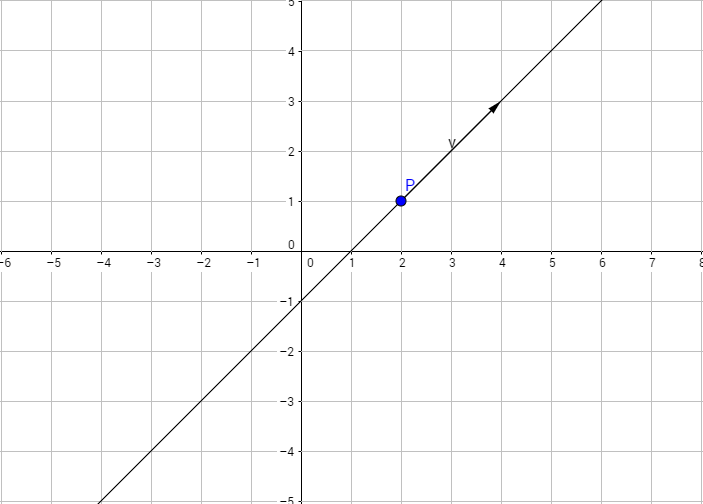
\includegraphics[width=\textwidth]{Graph1.png}\\
Eine Gerade ist genau dann ein UVR des \(\mathbb{R}^n\) falls \(0\in l(p,v)\).

\chapter{Lineare Unabhängigkeit und Basen}
\section{Definition}
Sei V ein K-Vektorraum und \((v_i)_{i\in I}\) eine Familie von Vektoren aus V. (d.h. \( I \neq \emptyset\) ist eine Menge und für alle \(i\in I\) gilt: \(v_i \in V\).
\begin{description}
\item[i)] v heißt \textbf{Linearkombination} von \((v_i)_{i\in I}\), falls es ein \(r \in \mathbb{N}\), \(i_1,\cdots,i_r \in I\) und \(\lambda_1,\cdots , \lambda_r \in K\) gibt mit \[v=\sum^{r}_{k=1}\lambda_k v_{i_k}.\]
Die Menge aller Linearkombinationen von \((v_i)_{i\in I}\) wird mit \(span((v_i)_{i\in I})\) notiert und heißt \textbf{Spann} von \((v_i)_{i\in I}\).\\
\textbf{Konvention:} \(span(\emptyset)=\{0\}\)
\item[ii)] \((v_i)_{i\in I}\) wird \textbf{Erzeugendensystem} von V genannt, falls  \(span((v_i)_{i\in I})= V\)
\item[iii)] V heißt \textbf{endlich erzeugt}, falls es ein \(r\in \mathbb{N}_0\) und \(v_1,\cdots v_r\in V\) so, dass \((v_1,\cdots , v_r)\) ein Erzeugendensystem von V ist.
\end{description}
\section{Bemerkung}
Sei \(U:=span((v_i)_{i\in I})\). Dann ist U ein UVR von V. Denn sind \(u_1,u_2 \in U\), so existiert \(r\in \mathbb{N}, i_1,\cdots , i_r \in I\) und \(\lambda^{(1)}_k,\lambda^{(2)}_k \in K \ (k=1,\cdots , r)\) mit:
\[
u_1=\sum^r_{k=1} \lambda^{(1)}_k v_{i_k},u_2=\sum^r_{k=1} \lambda^{(2)}_k v_{i_k}
\]
Somit folgt für alle \(\mu_1,\mu_2 \in K\):
\[
\mu_1 * u_1+ \mu_2 * u_2= \sum^r_{k=1} \underbrace{(\mu_1 \lambda^{(1)}_k + \mu_2 \lambda^{(2)}_k)}_{\in K} * v_{i_k} \in U
\]
\section{Beispiel}
\begin{description}
\item[i)] Für einen Körper K ist \(K^n\) endlich erzeugt. Sei:
\[
e_i=
\left(\begin{array}{c}
0\\
\vdots\\
0\\
1\\
0\\
\vdots\\
0
\end{array}\right) \leftarrow \text{i-te Position,}
\]
\textbf{i-te Einheitsvektor} im \(K^n\)(i=1,...,n). Dann ist \((e_1,...,e_n)\) ein Erzeugendensystem des \(K^n\), denn für alle \(x 
= \left(\begin{array}{c}x_1\\\vdots\\x_n\end{array}\right)\in K^n\) gilt: \[
x=\sum^n_{i=1}x_i*e_i
\]
\item[ii)] Der \(\mathbb{R}\)-VR der Polynomfunktion Pol(\(\mathbb{R}\)) ist nicht endlich erzeugt. Denn seinen \(p_1,...,p_n \in Pol(\mathbb{R})\) und \(\lambda_1,...,\lambda_n\) reelle Zahlen, sei k der maximale Grad dieser n-Polynome. Dann hat \[p:= \sum^n_{i=1}\lambda_i p_i\] höchstens Grad k. Also ist \((p_1,...,p_n)\) kein Erzeugendensystem von Pol(\(\mathbb{R}\)).
\end{description}
\section{Definiton}
Sei V ein K-VR.
\begin{description}
\item[i)] Eine endliche Familie von Vektoren \((v_1,...,v_n)\) wird \textbf{linear unabhängig} genannt, falls für alle \(\lambda_1,...,\lambda_n \in K\) gilt:\[ \sum^n_{i=1} \lambda_i v_i = 0\in V \Rightarrow \forall_{i=1,...,n}\lambda_i=0\in K\]
\item[ii)]Eine beliebige Familie von Vektoren \((v_i)_{i\in I}\) wird \textbf{linear unabhängig} genannt, falls jede endliche Teilfamilie linear unabhängig ist (d.h. für alle \(J \subset I\) endlich gilt: \((v_j)_{j\in J}\) ist linear unabhängig)\\
Andernfalls heißt \((v_i)_{i\in I}\) \textbf{linear abhängig}.
\item[iii)] Unter einer \textbf{Basis} von V verstehen wir ein linear unabhängiges Erzeugendensystem von V.
\end{description}
\section{Bemerkung}
Lineare Abhängigkeit bedeutet also, dass man aus der Familie \((v_i)_{i\in I}\) den Nullvektor durch eine nicht-triviale Linearkombination darstellen kann (d.h. durch eine Linearkombination, bei der nicht alle Koeffizienten gleich 0 sind).\\
Die Familie
\[
\left(
\left(
\begin{array}{c}
1\\0\\0
\end{array}
\right),
\left(
\begin{array}{c}
0\\1\\0
\end{array}
\right),
\left(
\begin{array}{c}
2\\2\\0
\end{array}
\right)
\right) \text{ im } \mathbb{R}^3
\]
ist also linear abhängig, denn 
\[-2*
\left(
\begin{array}{c}
1\\0\\0
\end{array}\right)
+(-2)*
\left(
\begin{array}{c}
0\\1\\0
\end{array}
\right)+1*
\left(
\begin{array}{c}
2\\2\\0
\end{array}
\right)
=\left(
\begin{array}{c}
0\\0\\0
\end{array}
\right)
\]
\section{Beispiele}
\begin{description}
\item[i)] Die Familie $(e_i)_{i=1,...,n}$ im $K^n$ ist eine Basis. Dann seien $\lambda_1,...,\lambda_n\in K$ mit
\[
\sum^n_{i=1}\lambda_ie_i =0 \in K^n
\]
Da $\sum^n_{i=1}\lambda_ie_i = \left(\begin{array}{c}
\lambda_1\\
\vdots\\
\lambda_n
\end{array}\right)$, folgt $\lambda_i=0\in K$ für alle i=1,...,n. Also ist ($e_i,...,e_n$) linear unabhängig. Nach Beispiel 3.3 ist ($e_i,...,e_n$) auch ein Erzeugendensystem, also eine Basis.\\
($e_i,...,e_n$) wird \textbf{kanonische Basis} in $K^n$ genannt.
\item[ii)] Die Familie $\left(\left(\begin{array}{c}1\\0\\0\end{array}\right),\left(\begin{array}{c}1\\2\\0\end{array}\right),\left(\begin{array}{c}1\\2\\3\end{array}\right)\right)$ ist eine Basis im $\mathbb{R}^3$\\
Lineare Unabhängigkeit:
\[
\lambda_1 * \left(\begin{array}{c}1\\0\\0\end{array}\right) +\lambda_2 *\left(\begin{array}{c}1\\2\\0\end{array}\right)+\lambda_3*\left(\begin{array}{c}1\\2\\3\end{array}\right) = \left(\begin{array}{c}0\\0\\0\end{array}\right)
\]
\[
\Rightarrow 3*\lambda_3 = 0 \Rightarrow \lambda_3 = 0
\]
\[
\Rightarrow \lambda_1 *\left(\begin{array}{c}1\\0\\0\end{array}\right) +\lambda_2 *\left(\begin{array}{c}1\\2\\0\end{array}\right) = \left(\begin{array}{c}0\\0\\0\end{array}\right) \Rightarrow \lambda_2=0\Rightarrow \lambda_1=0.
\]
Erzeugendensystem:
Sei $x =\left(\begin{array}{c}x_1\\x_2\\x_3\end{array}\right)\in \mathbb{R}^3 $.\\Dann $\lambda_1 * \left(\begin{array}{c}1\\0\\0\end{array}\right) +\lambda_2 *\left(\begin{array}{c}1\\2\\0\end{array}\right)+\lambda_3*\left(\begin{array}{c}1\\2\\3\end{array}\right) = \left(\begin{array}{c}x_1\\x_2\\x_3\end{array}\right)$\\für $\lambda_3 = \dfrac{x_3}{3},\ \lambda_2 = \dfrac{x_2}{2}-\dfrac{x_3}{3},\  \lambda_1 = x_1-\dfrac{x_2}{2}$.
\item[iii)] Seien $q_n(t)=t^n,n\in \mathbb{N}_0$. Dann ist $(q_n)_{n\in \mathbb{N}_0}$ eine Basis von Pol($\mathbb{R}$).\\
Lineare Unabhängigkeit:  Sei $n \in \mathbb{N}$ beliebig. Ist $\lambda_i \neq 0$ für ein $i=0,...,n$, dann hat 
\[
\left(
\sum^n_{i=0}q_i
\right)(t)=\sum^n_{i=0}\lambda_i t^i
\]
höchstens n Nullstellen. Also ist $\sum^n_{i=0}\lambda_i q_i \neq 0 \in Pol(\mathbb{R})$.\\
Erzeugendensystem: Sei $p\in Pol(\mathbb{R})$. Dann
\[
p(t) = \sum^n_{k=0}\lambda_k t^k \text{ für ein }n\in \mathbb{N}_0, \lambda_1,...,\lambda_n \in \mathbb{R.} 
\]
\[
\text{Also } p=\sum^n_{k=0} \lambda_kq_k.
\]
\end{description}
Zur Charakterisierung von Basen:
\section{Satz}
Sei \textit{B} = $(v_1,...,v_n)$ eine Familie von Vektoren eines K-VR V. Dann sind äquivalent:
\begin{description}
\item[i)] \textit{B} ist Basis
\item[ii)] \textit{B} ist ein unverkürzbares Erzeugendensystem, das heißt für jedes $r\in \{1,...,n\}$ ist $(v_1,...,v_{r-1},v_{r+1},...,v_n)$ kein Erzeugendensystem, aber \textit{B} ist Erzeugendensystem.
\item[iii)] Zu jedem Vektor $v\in V$ ex. eindeutig bestimmte $\lambda_1,...,\lambda_n \in K$ mit: $v=\sum^n_{i=0}\lambda_iv_i$
\item[iv)] \textit{B} ist unverlängerbar linear unabhängig, d.h. \textit{B} ist linear unabhängig und für alle $v \in V$ ist $(v_1,...,v_n,v)$ linear abhängig.
\end{description}
\subsection*{Beweis:}
\begin{description}
\item[i) $\Rightarrow$ ii):] Sei \textit{B} ein Erzeugendensystem. Ist \textit{B} verkürzbar, so gilt:
\[
v_r = \lambda_1 v_1+...+\lambda_{r-1} v_{r-1}+\lambda_{r+1} v_{r+1}+...+\lambda_nv_n
\] 
Also:
\[
\lambda_1 v_1+...+\lambda_{r-1} v_{r-1}+\lambda_{r+1} v_{r+1}+...+\lambda_nv_n+(-1)*v_r=0,
\] d.h. \textit{B} ist nicht linear unabhängig und also keine Basis.
\item[ii)$\Rightarrow$ iii):] Sei \textit{B} ein Erzeugendensystem. Ist die Eindeutigkeitsbedingung nicht erfüllt, so gibt es ein $v \in V$ mit 
\[
v=\lambda_1v_1,...,\lambda_nv_n=\mu_1v_1+...+\mu_nv_n
\]
($\lambda_r\neq \mu_r$ für mindestens ein $r$).\\
Für ein solches $r$ gilt:
\[
v_r=\dfrac{\mu_1-\lambda_1}{\lambda_r-\mu_r}v_1+...+\dfrac{\mu_{r-1}-\lambda_{r-1}}{\lambda_r-\mu_r}v_{r-1}+\dfrac{\mu_{r+1}-\lambda_{r+1}}{\lambda_r-\mu_r}v_{r+1}+...+\dfrac{\mu_n-\lambda_n}{\lambda_r-\mu_r}v_n
\]
Also ist \textit{B} verkürzbar.
\item[iii) $\Rightarrow$ iv):] Aus iii) mit $v=0\in V$ folgt direkt die lineare Unabhängigkeit. Sei $v\in V $. Dann hat v die Darstellung:
\[
v=\sum^n_{i=1}\lambda_iv_i
\]
Also
\[
\sum^n_{i=1}\lambda_1v_i +(-1)*v = 0,
\]
d.h. $(v_1,...,v_n,v)$ ist linear abhängig.
\item[iv) $\Rightarrow$ i):] Aus iv) folgt: Für jedes $v\in V$ existieren $\lambda_1,...,\lambda_n,\lambda \in K$ mit \[
\sum^n_{i=1}\lambda_i\lambda v = 0,
\]
wobei nicht alle $\lambda_1,...,\lambda_n, \lambda$ gleich 0 sind. Da \textit{B} linear unabhängig ist, muss gelten $\lambda\neq 0$. Also:
\[
v=\sum^n_{i=1}\dfrac{-\lambda_1}{\lambda}v_i,
\]
d.h. \textit{B} ist auch ein Erzeugendensystem. $_\square$
\end{description}
\section{Folgerung}
Jeder endlich erzeugte K-VR hat eine Basis.
\subsection*{Beweis:}
Von einem endlichen Erzeugendensystem nehme man so lange Vektoren weg, bis es unverkürzbar ist. $_\square$
\subsection*{Konvention:}
Die leere Familie von Vektoren ist linear unabhängig, also ist sie Basis von $V=\{0\}$.
\subsection*{Frage:}
Kann ein endlich erzeugter Vektorraum Basen unterschiedlicher Länge (also mit unterschiedlich vielen Vektoren) haben?
\section{Lemma (Austauschlemma)}
Sei V ein K-VR mit Basis \textit{B}$=(v_1,...,v_n)$ und $w=\sum^n_{k=1}\lambda_kv_k \in V$.\\
Falls $\lambda_k \neq 0$, so ist $(v_1,...,v_{k-1},w,v_{k+1},...,v_n) =:$\textit{B}' ebenfalls eine Basis von V.
\subsection*{Beweis:}
Durch Umnummerierung kann man erreichen, dass $k=1$. \begin{itemize}
\item \textit{B}'$=(w,v_2,...,v_n)$ ist Erzeugendensystem:\\
Sei $v\in V$. Dann: $v= \sum^n_{i=1}\mu_iv_i,\mu_1,...,\mu_n \in K$. Da $\lambda_1\neq 0$, folgt:
\[
v_1=\dfrac{1}{\lambda_1}w-\sum^n_{i=2}\dfrac{\lambda_i}{\lambda_1}v_i
\]
Somit:
\[
v=\dfrac{\mu_1}{\lambda_1}w+\sum^n_{i=2} (\mu_i-\dfrac{\mu_1}{\lambda_1}\lambda_i)v_i
\]
\item \textit{B}' ist linear unabhängig: Sei
\[
0=\mu * w + \sum^n_{i=2}\mu_i v_i
\]
Da $w=\sum^n_{i=1}\lambda_iv_i$, folgt:
\[
0=\mu \lambda_1 v_1 +\sum^n_{i=2}(\mu_i+\mu\lambda_i)v_i
\]
Da \textit{B} linear unabhängig ist, folgt: $\mu\lambda_1 = 0$ und $(\mu_i+\mu\lambda_i)=0$ für $i=2,...,n$.\\
Da $\lambda_1\neq 0$, gilt $\mu = 0$ und $\mu_i=0$ für $i=2,...,n$.$_\square$
\end{itemize}
\section{Satz}
Sei V ein K-VR mit Basis \textit{B}$=(v_1,...,v_r)$ und $(w_1,...,w_n)$ eine linear unabhängige Familie in V. Dann:
\begin{description}
\item[i)]$n\leq r$
\item[ii)] Es gibt Indizes $i_1,...,i_n\in \{1,...,r\}$, sodass die Familie \textit{B}', die entsteht, wenn man in \textit{B} $v_{i_1},...,v_{i_n}$ durch $w_1,...,w_n$ ersetzt, weiterhin eine Basis von V ist.
\end{description}
\subsection*{Beweis:}
Induktion über $n \in \mathbb{N}_0$
\begin{itemize}
\item $n=0$: Hier ist nichts zu zeigen
\item $(n-1)\rightsquigarrow n:$ Da auch $(w_1,...,w_{n-1})$ linear unabhängig ist, ergibt die Induktionsannahme, dass $(n-1)\leq r$ und dass nach geeigneter Umnummerierung der Basis \textit{B} $(w_1,...,w_{n-1},v_n,...,v_r)$ Basis von V ist (Umnummerierung mit $i_1=1,...,i_{n-1}=n-1$).\\
Um $n\leq r$ zu zeigen, genügt es, $n-1=r$ zu einem Widerspruch zu führen. In diesem Fall wäre $(w_1,...,w_{n-1})$ eine Basis von V im Widerspruch zu Satz 3.7 iv).\\
Ferner hat $w_n$ die Darstellung
\[
w_n=\lambda_1w_1+...+\lambda_{n-1}w_{n-1}+\lambda_nv_n+...+\lambda_rv_r
\]
Da $(w_1,...,w_n)$ linear unabhängig ist, folgt $\lambda_k \neq 0$ für ein $k=n.n+1,...,r$. Also kann nach dem Austauschlemma $v_k$ durch $w_n$ ersetzt werden, ohne dass die Basiseigenschaft verloren geht.$_\square$
\end{itemize}
\section{Folgerung}
Sei V ein K-VR mit Basen $(v_1,...,v_n)$ und $(w_1,...,w_r)$. Dann: $n=r$.
\subsection*{Beweis}
Der Austauschsatz liefert: $n\leq r$ und $r\leq n$. $\square$
\section{Folgerung}
Hat ein K-VR eine endliche Basis, so sind alle seine Basen endlich.
\subsection*{Beweis}
Sei $(v_1,...,v_r)$ eine endliche Basis und $(w_i)_{i\in I}$ eine unendliche Basis. Dann existiert $i_1,...,i_{r+1}\in I$ mit $(w_{i_1},...,w_{i_{r+1}})$ linear unabhängig ist. Dies widerspricht dem Austauschsatz. $_\square$\\\\
Also ist der folgende Dimensionsbegriff wohldefiniert.
\section{Definition}
Ist V ein K-VR, so definieren wir die \textbf{Dimension} von V durch:
\[
dimV=\left\{\begin{array}{cl}
\infty &\text{, falls V nicht endlich erzeugt}\\
r&\text{, falls V Basis der Länge } r \in \mathbb{N}_0\text{ hat.}
\end{array}\right.
\]
Hierbei sei die \textbf{Länge} einer endlichen Basis die Anzahl von Vektoren in der Basis. Man schreibt auch $dim_KV$ statt $dimV$, falls der Körper aus dem Kontext nicht klar ist.
\section{Beispiel}
\begin{description}
\item[i)] $dimK^n=n$
\item[ii)] $dim Pol(\mathbb{R}) = \infty$
\end{description}
\section{Beispiel (und Erinnerung)}
Auf dem $\mathbb{R}^2$ führen wir folgende Multiplikation ein:
\[*:\mathbb{R}^2\times \mathbb{R}^2 \rightarrow \mathbb{R}^2:\]
\[\left(\left(
\begin{array}{c}
x_1\\x_2
\end{array}
\right),\left(
\begin{array}{c}
y_1\\y_2
\end{array}
\right)\right)\mapsto \left(
\begin{array}{ccc}
x_1y_1&-&x_2y_2\\
x_1y_2&+&x_2y_1
\end{array}
\right)\]
Mit diesem Beispiel wird $(\mathbb{R},+,*)$ zu einem Körper, dem Körper der \textbf{komplexen Zahlen}, $\mathbb{C}$. Das neutrale Element bzgl.$*$ ist $\left(
\begin{array}{c}
1\\0
\end{array}
\right)$.
Man notiert daher:
\[
1:=\left(\begin{array}{c}1\\0\end{array}\right), i:= \left(\begin{array}{c}0\\1\end{array}\right)
\]
Jedes $z\in \mathbb{C}$ hat dann eine eindeutige Darstellung der Form:
\[
z=\lambda_1*1+\lambda_2*i, \lambda_1,\lambda_2 \in \mathbb{R}
\]
$\lambda_1$ heißt \textbf{Realteil} von $z (Re(z))$, $\lambda_2$ \textbf{Imaginärteil} von $z (Im(z))$. i wird \textbf{imaginäre Einheit} genannt. Es gilt:
\[
i^2=i*i=-1\in\mathbb{C}
\]
Die reellen Zahlen können als Teilmenge von $\mathbb{C}$ aufgefasst werden, indem man $\lambda \in\mathbb{R}$ mit der komplexen Zahl $\lambda*1\in\mathbb{C}$ identifiziert. (Die reellen Zahlen findet man also auf der x-Achse). Man schreibt dann: $z=\lambda_1+\lambda_2*i$ als Kurzform für $z=\lambda_1*1+\lambda_2*i\ (\lambda_1,\lambda_2\in \mathbb{R})$
Nach Beispiel 3.14 gilt:
\[
dim_{\mathbb{C}}\mathbb{C}=1
\]
\[
dim_{\mathbb{R}}\mathbb{C}=dim_{\mathbb{R}}\mathbb{R}^2=2
\]
Einige weiter Folgerungen des Austauschsatzes:
\section{Folgerung(Basisergänzungssatz)}
Sei V ein endlich erzeugter K-VR und $(v_1,...,v_n)$ linear unabhängig. Dann existiert $r\in\mathbb{N}_0$ und $v_{n+1},...,v_{n+r}\in V$, sodass $(v_1,...,v_{n+r})$ eine Basis von V ist.
\section{Folgerung}
Ist U ein UVR eines endlich erzeugten K-VR V. Dann:\begin{description}
\item[i)]$dimU\leq dimV$
\item[ii)]$dimU=dimV\Rightarrow U=V$
\end{description}
\chapter{Matrizen}
Sei K ein Körper. Wir bezeichnen mit $k^{m\times n}$ die Menge aller $m \times n$-Matrizen mit Einträgen in K, also der Rechteckschemata der Form:\[
A=(a_{ij})_{i=1,...,m,j=1,...,n}=
\left(
\begin{array}{ccc}
a_{11}&\cdots&a_{1n}\\
\vdots&\ddots&\vdots\\
a_{m1}&\cdots&a_{mn}
\end{array}
\right)
,a_{ij}\in K.
\]
Mit  Addition:
\[
(a_{ij})_{i=1,...,m,j=1,...,n}+(b_{ij})_{i=1,...,m,j=1,...,n}:=(a_{ij}+b_{ij})_{i=1,...,m,j=1,...,n}
\]
und der skalaren Multiplikation:
\[
\lambda*(a_{ij})=(\lambda*a_{ij}), \lambda\in K
\]
wird $K^{m\times n}$ zu einem K-VR.
\section{Definition}
Sei $A \in K^{m \times n}$ mit Zeilen:\[
a_1:=
\left(
\begin{array}{c}
a_{11}\\\vdots\\a_{1n}
\end{array}
\right)
,...,
a_m:=
\left(
\begin{array}{c}
a_{m1}\\\vdots\\a_{mn}
\end{array}
\right)
\]
(als Spaltenvektor geschrieben). Dann wird $Z(A) := span(a_1,...,a_m) \subset K^n$ der \textbf{Zeilenraum} von A genannt.
\section{Algorithmus}
\begin{description}
\item[Input:] $A \in K^{m \times n}$
\item[Output:] Basis \textit{B} von $Z(A)$
\begin{description}
\item[1.:] Bringe A auf Zeilenstufenform mit Algorithmus 1.6 und bezeichne die resultierende Matrix mit $\tilde{A}=(\tilde{a}_{ij})_{i=1,...,m,j=1,...,n}$ 
\item[2.:] Bestimme den Zeilenrang r von $\tilde{A}$ (also die Anzahl von Zeilen von $\tilde{A}$, die nicht nur Nulleinträge haben).
\item[3.:] Setze für $i = 1,...,r$
\[
b_i=\left(
\begin{array}{c}
\tilde{a}_{i1}\\\vdots\\\tilde{a}_{in}
\end{array}
\right)\text{(i-te Zeile von }\tilde{A}\text{ als Spaltenvektor)}
\]
und gebe \textit{B}$=(b_1,...,b_r)$ aus.
\end{description}
\end{description}
\subsection*{Beweis der Korrektheit von Algorithmus 4.2}
\begin{description}
\item[i)] Elementare Zeilenumformungen ändern den Zeilenraum nicht, d.h. $Z(A)=Z(\tilde{A})$. Ist etwa $v\in Z(A)$ und $A_1$ gehe aus $A$ hervor, indem das $\lambda$-fache der j-ten Zeile zur i-ten Zeile addiert wird. Dann:
\[
v=\sum^m_{k=1}\mu_ka_k=\left(\sum_{k\in \{1,...,m\}\backslash\{i,j\}} \mu_ka_k \right)+\mu_i(a_i+\lambda a_j)+(\mu_i-\lambda\mu_i)a_j
\]
Also $v\in Z(A_1)$, d.h. $Z(A)\subset Z(A_1)$\\
Analog: $Z(A_1)\subset Z(A)$\\
klar: Zeilenvertauschungen ändern den Zeilenraum nicht.
\item[ii)] \textit{B} ist Erzeugendensystem von $Z(A)$:\\
Dies folgt aus i), da \textit{B} ein Erzeugendensystem von $Z(\tilde{A})$ (Weglassen der Nullzeilen ändert den Spann nicht).
\item[iii)] $B$ ist linear unabhängig:\\
Sei $\tilde{a}_{i,j_i}$ der i-te Pivot von $\tilde{A}$. Dann:\[
\tilde{a}_{k,j_1} = 0 \ \forall k >i.
\]
Seien $\lambda_1,...,\lambda_r \in K$ mit 
\[
\lambda_1 b_1+...+\lambda_r b_r = 0 \in K^n
\]
Betrachtung des $j_1$-ten Eintrags führt zu\[
\lambda_1\underbrace{\tilde{a}_{1,j_1}}_{\neq 0}+\lambda_2\underbrace{\tilde{a}_{2,j_1}}_{=0}+...+\lambda_r\underbrace{\tilde{a}_{r,j_1}}_{=0} = 0 \in K
\]
Also: $\lambda_1=0$. Iteriert man dies, folgt leicht: $\lambda_k=0 \  \forall k=1,...,r$. $_\square$ 
\end{description}
\section{Bemerkung}
Die Algorithmen 1.3, 1.6, 1.8 behalten ihre Gültigkeit, falls man $\mathbb{R}$ durch einen beliebigen Körper K ersetzt. Spezielle Eigenschaften wurden dort nicht verwendet.
\section{Bemerkung}
Man nennt die Dimension des Zeilenraums einer Matrix $A\in K^{m\times n}$ den \textbf{Zeilenrang} von $A$. Für Matrizen in Zeilenstufenform stimmt dies mit der Begriffsbildung aus Definition 1.2 überein. Die Zahl r im Output von Algorithmus 1.8 ist also der Zeilenrang von A, da elementare Zeilenumformungen den Zeilenrang nicht ändern.
\section{Beispiel}
Sei
\[
U =span
\left(
\left(
\begin{array}{c}
0\\0\\1\\2\\9
\end{array}
\right),
\left(
\begin{array}{c}
0\\3\\4\\5\\9
\end{array}
\right),
\left(
\begin{array}{c}
0\\6\\7\\8\\9
\end{array}
\right),
\left(
\begin{array}{c}
0\\9\\9\\9\\9
\end{array}
\right)
\right) \subset \mathbb{R}^5
\]
Wir betrachten:
\[
A=
\left(
\begin{array}{ccccc}
0&0&1&2&9\\
0&3&4&5&9\\
0&6&7&8&9\\
0&9&9&9&9
\end{array}
\right)
\]
Algorithmus 1.6 liefert(s. Beispiel 1.7):
\[
\tilde{A}=
\left(
\begin{array}{ccccc}
0&3&4&5&9\\
0&0&1&2&9\\
0&0&0&0&9\\
0&0&0&0&0
\end{array}
\right)
\]
Also ist $dim(Z(A))=3$ und 
\[
U =span
\left(
\left(
\begin{array}{c}
0\\3\\4\\5\\9
\end{array}
\right),
\left(
\begin{array}{c}
0\\0\\1\\2\\9
\end{array}
\right),
\left(
\begin{array}{c}
0\\0\\0\\0\\9
\end{array}
\right)\right) \text{ist Basis von }Z(A).
\]
\section{Definition}
Seien $A=(a_{ij})\in K^{m \times n}$ und $B=(b_{jk})\in K^{m \times r}$ (d.h. A hat so viele Spalten, wie B Zeilen). Dann ist das Produkt von A und B definiert durch
\[
A\cdot B := C \in K^{m\times r}, C=(c_{ik})_{i=1,...,m,k=1,...,r}
\]
\[
c_{ik} := \sum^n_{j=1}a_{ij}b_{jk}
\]
$A\cdot B$ hat also so viele Zeilen wie A und so viele Spalten wie B.
\[
\left(
\begin{array}{ccccc}
\cdot&\cdot&\cdot&\cdot&\cdot\\
a_{i1}&a_{i2}&\cdot&\cdot&a_{in}\\
\cdot&\cdot&\cdot&\cdot&\cdot\\
\cdot&\cdot&\cdot&\cdot&\cdot\\
\end{array}
\right) 
\left(
\begin{array}{ccc}
\cdot&b_{1k}&\cdot\\
\cdot&b_{2k}&\cdot\\
\cdot&\cdot&\cdot\\
\cdot&\cdot&\cdot\\
\cdot&b_{rk}&\cdot\\
\end{array}
\right)=\left(
\begin{array}{ccc}
\cdot&\cdot&\cdot\\
\cdot&a_{ik}&\cdot\\
\cdot&\cdot&\cdot\\
\cdot&\cdot&\cdot\\
\end{array}
\right)
\]
\section{Bemerkung}
Die Matrixmultiplikation ist nicht kommutativ, selbst dann nicht, wenn $AB$ und $BA$ definiert werden können (d.h. $A\in K^{m\times n}, b\in K^{n\times m}$).
\subsection*{Gegenbeispiel}
\[
\left(
\begin{array}{cc}
1&0\\
0&0\\
\end{array}
\right) \cdot
\left(
\begin{array}{cc}
0&1\\
0&0\\
\end{array}
\right) = 
\left(
\begin{array}{cc}
0&1\\
0&0\\
\end{array}
\right)
\]
\[
\left(
\begin{array}{cc}
0&1\\
0&0\\
\end{array}
\right) \cdot
\left(
\begin{array}{cc}
1&0\\
0&0\\
\end{array}
\right) = 
\left(
\begin{array}{cc}
0&0\\
0&0\\
\end{array}
\right)
\]
Wir bezeichnen mit $E_n$ die n-reihige Einheitsmatrix, d.h.:
\[
E_n := \left(
\begin{array}{ccc}
1&&0\\
&\ddots&\\
0&&1\\
\end{array}
\right)\in K^{n\times n}
\]\\
Die folgenden Rechenregeln können elementar überprüft werden:
\section{Satz}
Seien $A,A' \in K^{m \times n},B,B' \in K^{n\times r},C \in K^{r \times s}$ und $\lambda \in K$, dann:
\begin{description}
\item[i)] $A\cdot(B+B') = A\cdot B + A\cdot B'$ und $(A+A')\cdot B = A\cdot B + A' \cdot B$ (Distributivgesetze)
\item[ii)] $(A\cdot B)\cdot C = A\cdot (B\cdot C)$ (Assoziativgesetz)
\item[iii)] $E_m \cdot A = A\cdot E_n$
\item[iv)] $A\cdot (\lambda B) = (\lambda A)\cdot B = \lambda (A\cdot B)$
\end{description}
\section{Bemerkung}
\begin{description}
\item[i)] Man schreibt auch $AB$, statt $A\cdot B$
\item[ii)]Eine Matrix mit n Zeilen und 1 Spalte ist ein Spaltenvektor der Höhe n. Man schreibt $K^n$, statt $K^{n\times 1}$. Als Spezialfall von Definition 4.6 erhält man:\[
A*x=\left(
\begin{array}{c}
\sum^n_{j=1}a_{1j}x_j\\
\vdots\\
\sum^n_{j=1}a_{mj}x_j\\
\end{array}
\right), x= \left(
\begin{array}{c}
x_1\\\vdots\\x_n
\end{array}
\right) \in K^n
\]
Analog werden Elemente von $K^{1\times n}$ werden \textbf{Zeilenvektoren genannt}
\end{description}
\section{Satz}
Sei $A\in K^{m \times n}$ und $b \in K ^m$. Dann sind äquivalent:
\begin{description}
\item[i)] Lös$(A,b)\neq \emptyset$, d.h. es existiert eine Lösung zu $Ax=b$ 
\item[ii)] Zeilenrang(A) = Zeilenrang((A,b))
\end{description}
\subsection*{Beweis}
Wir verwenden den Algorithmus 1.8 und Bemerkung 4.3 und 4.4.\\
Sei \\$r :=$ Zeilenrang($\tilde{A}$). Da Zeilenrang(A) = Zeilenrang ((A,b))\\ $\Leftrightarrow$ Zeilenrang($\tilde{A}$) = Zeilenrang(($\tilde{A},\tilde{b}$)) \\$\Leftrightarrow$ Die Gleichungen $r+1,...,m$ von $\tilde{A}x = \tilde{b}$ lauten $0=0$ \\$\Leftrightarrow$ Algorithmus 1.8 liefert mindestens eine Lösung zu $Ax=b$.
\section{Satz}
Sei $A \in K^{m\times n}$, $b \in K^m$. Dann sind äquivalent:
\begin{description}
\item[i)] Lös$(A,b)$ hat höchstens ein Element, d.h. es gibt höchstens eine Lösung $x \in K^n $ zu $Ax=b$
\item[ii)] Zeilenrang$(A)=n$
\end{description}
\subsubsection*{Beweis}
Nach Bemerkung 4.4 folgt: Zeilenrang(A)= n $\Leftrightarrow$ Algorithmus 1.8 liefert "`keine Lösung"' oder Bijektion $\Phi_{A,B}:\mathbb{R}^{n-r} \rightarrow \text{Lös}(A,b) \Rightarrow \text{Lös}(A,b)$ höchstens 1 Element.
\section{Definition}
Eine Matrix $A\in K^{n \times n}$ wird \textbf{invertierbar} genannt, falls ein $B \in K^{n\times n}$ existiert mit $B\cdot A = E_n$.Wir bezeichnen mit $GL(n,k)$ die Menge aller invertierbaren Matrizen in $k^{m\times n}$ (GL $\Leftrightarrow$ "`general linear"').
\section{Satz}
Sei $A\in K^{n\times n}$. Dann sind äquivalent:
\begin{description}
\item[i)] $\forall b \in K^n: Ax=b$ hat genau eine Lösung $x\in K^n$
\item[ii)] Lös$(A,0) = \{0\}$
\item[iii)] Zeilenrang(A) = n
\item[iv)] Die Spalten von A bilden eine Basis in $K^n$
\item[v)] A ist invertierbar, d.h. es ex. $B \in K^{n\times n}$  mit $B\cdot A = E_m$\\In diesem Fall gilt: B ist eindeutig bestimmt und $B \in GL(n,K)$. Man nennt B die \textbf{Inverse} von A und schreibt $A^{-1}$ statt B.
\end{description}
\textbf{Zur Vorbereitung}:
\section{Definition}
Sei $A=(a_{ij}) \in K^{m \times n}$. Dann wird die durch :\[
A^T=(a'_{ji})_{j=1,...,n,i=1,...,m},(a_{ij}) =: (a'_{ji})
\]
definierte Matrix $\in K^{n\times m}$ die \textbf{Transponierte} von A genannt. Hier wird also die i-te Zeile von A zur i-ten Spalte von $A^T$.\\
\\
Man prüft leicht: $\forall A \in K^{m \times n} , B \in K^{n \times r}$
\[
(A^T)^T = A \text{ und } (AB)^T = B^T A^T
\]
\section{Bemerkung}
Unter dem Spaltenraum von $A \in K^{m \times n}$ versteht man den von den Spalten einer Matrix aufgespannten U-VR von $K^m$. Dies ist nach Definition identisch mit dem Zeilenraum von $A^T$. Seine Dimension wird \textbf{Spaltenrang} von A genannt.\\\\Bedingung iv) in Satz 4.13 ist äquivalent zu iv') Spaltenrang$(A)=n$\\Später sehen wir: Es gilt stets: Zeilenrang(A) = Spaltenrang(A).\\\\
\textbf{Beweis von Satz 4.13:} Wir zeigen $iii) \Rightarrow ii) \Rightarrow iv) \Rightarrow v) \Rightarrow iii) $ und $i) \Leftrightarrow iv)$
\begin{description}
\item[iii) $\Rightarrow$ ii)] Nach Satz 4.11 hat Lös(A,0) höchstens ein Element. \\Da stets $A\left(
\begin{array}{c}
0\\\vdots\\0
\end{array}
\right)=\left(
\begin{array}{c}
0\\\vdots\\0
\end{array}
\right)$, folgt: Lös(A,0)=\{0\}
\item[ii) $\Rightarrow$ iv)] Sei $a_{\cdot i}$ die i-te Spalte von A, $x \in K^n$.\\
Dann $Ax=\sum^m_{i=1} x_i a_{\cdot i}$\\
\textbf{ii)} $\\Leftrightarrow$ Lös$(A,b)=\{0\} \Leftrightarrow Ax=0$ gilt nur für $x_1=...=x_n=0$\\$ \Leftrightarrow x_1 a_{\cdot 1} +...+ x_n a_{\cdot n}=0$ nur für $x_1=...=x_n=0$\\$ \Leftrightarrow a_{\cdot 1},...,a_{\cdot n} $ sind linear unabhängig.\\
Da alle Basen des $K^n$ die Länge n haben (Folgerung 3.11) ist $(a_{\cdot 1},...,a_{\cdot n})$ nach Satz 3.10 unverlängerbar linear unabhängig, also eine Basis von $K^n$ (Satz 3.7)
\item[iv) $\Leftrightarrow$ i)] Da $Ax=b \Leftrightarrow x_1a_{\cdot 1} + \cdots + x_na_{\cdot n} = b$, liefert Satz 3.7 die Äquivalenz von iv) und i) (vgl. Folien).
\item[iv) $\Rightarrow$ v)] Nach Bemerkung 4.13 ist dann Zeilenrang$(A^T)=n$ und so ist auch Zeilenrang$(A^T|b)=n \ \forall b\in K^n$.\\
Satz 4.10 liefert: $\forall b \in K^n$ existiert eine Lösung $x\in K^n$ zu $A^Tx=b$. Für $i=1,...,n$ wähle $b:=e_i=\left(
\begin{array}{c}
0\\\vdots\\0\\1\\0\\\vdots\\0
\end{array}
\right) \leftarrow \text{i-te Zeile}$. Dann existieren $c_{\cdot i} \in K^n$ mit $A^T c_{\cdot i} = e_i$. Die Matrix C mit Spalten $c_{\cdot i}$ erfüllt dann\[A^T * C = E_n\] Sei $B := C^T$, dann gilt: \\$B\cdot A=((B\cdot A)^T)^T = ((C^T\cdot A)^T)^T=(A^T \cdot C)^T = (E_n)^T = E_n \\\Rightarrow$ A ist invertierbar.
\item[v) $\Rightarrow$ iii)] Sei C wie oben, d.h. $C = B^T$, dann: \\$A^TC=A^TB^T=(BA)^T = E_n^T =E_n$ $\Rightarrow \ \forall x \in K^n$ gilt:\\\[\begin{array}{ccc}
(A^TC)x&=&E_nx\\
\parallel&&\parallel\\
A^T(Cx)&=&x\\
&&\Downarrow
\end{array}\]\\
$ \forall x \in K^n$ ist darstellbar als lineare Kombination von Spalten der $A^T$ (mit Koeffizienten$(Cx)$). Somit erzeugen die Spalten von $A^T$ und also die Zeilen von $A$ den $K^n$. Da $dim K^n =n$ und $A$ $n$ Zeilen hat, bilden die Zeilen von $A$ ein unverkürzbares Erzeugendensystem, also eine Basis von $K^n$ (Satz 3.7). Somit ist Zeilenrang$(A)=n$.$_square$
\end{description}
\textbf{Zusatz:} Sei $A \in K^{n\times n}$ invertierbar, d.h. $\exists B\in K^{n \times n}$ mit $B\cdot A = E_n$. Wir zeigen, dass B eindeutig bestimmt und invertierbar ist. Sei $B\cdot A = E_n$. Dann gilt für alle $x \in K^n$: $(BA)x=E_nx \Leftrightarrow B(Ax)=x$. Also erzeugen die Spalten von $B$ den $K^n$. Da $dim K^n = n$ und $B$ $n$ Spaten hat, bilden die Spalten von $B$ ein unverkürzbares Erzeugendensystem, und also eine Basis von $K^n$. Nach Satz 4.13(iv)$\Leftrightarrow$ v)) folgt, dass $B$ invertierbar ist. Die Eindeutigkeit von $B$ ergibt sich aus Satz 2.3 und dem folgenden Satz:
\section{Satz}
$GL(n,k)$ bildet versehen mit der Matrixmultiplikation eine Gruppe.
\subsection*{Beweis}
\begin{itemize}
\item Seien $A,B \in GL(n,K)$. Dann existieren $A',B' \in GL(n,K)$ mit $A'A =E_n, B'B=E_n$. Ferner, $(B'A')AB = B'\underbrace{(A'A)}_{=E_n}B = B'B = E_n$. Also: $AB \in GL(n,K)$.
\item Assoziativität: Folgt aus Satz 4.8.
\item Neutrales Element: $E_n$
\item Inverses Element: $A\in GL(n,K)\Rightarrow \exists A'\in GL(n,K)$ mit $A'A = E_n \Rightarrow A'$ ist Inverse zu A. $\square$
\end{itemize}
\section{Bemerkung}
\begin{description}
\item[i)] Ist A invertierbar, so gilt nach Satz 2.3: $A^{-1} A = A A^{-1} = E_n$
\item[ii)] Ist A invertierbar, so ist auch $A^T$ invertierbar. Und es gilt: $(A^T)^{-1} = (A^{-1})^T$. Denn: $(A^{-1})^T A^T = (A A^{-1})^T = (E_n)^T = E_n$
\end{description}
\subsection*{Zur Berechnung der Inversen:}
Nach Bem 4.17 i) und Satz 4.13 gilt: Ist A invertierbar, so $\exists A^{-1}$ mit $AA^{-1}= E_n$.\\ Sei $A^{-1} = \left( \begin{array}{ccc}
x_{11}&\cdots &x_{1n}\\
\vdots& \ddots & \vdots\\
x_{n1}&\cdots &x_{nn}\\
\end{array} \right)$, dann für jedes $i=1,...,n$ ist $x_{\cdot i}:=\left(\begin{array}{c}
x_{1i}\\ \vdots \\ x_{ni}
\end{array}\right)
$ die eindeutige Lösung zu $Ax=e_{i}$.
\subsection*{Man geht also wie folgt vor:}
\begin{description}
\item[i)] Betrachte die erweiterte $n\times (2n)$ Matrix $(A|\underbrace{ E_n}_{e_1...e_n})$ und bringe diese mit Algorithmus 1.6 auf Zeilenstufenform: $(A|E_n) \rightsquigarrow (\tilde{A}|\tilde{B})$
\item[ii)] Ist Zeilenrang von $\tilde{A} <n$ (d.h. hat $\tilde{A}$ eine Nullzeile), so ist A nicht invertierbar.
\item[iii)] Andernfalls hat $(\tilde{A}|\tilde{B})$ die Form: \\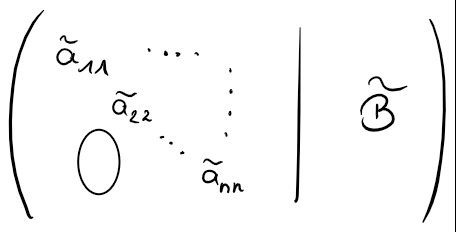
\includegraphics{Matrix_1} mit $\tilde{a}_{ii} \neq 0 \ \forall i = 1,...,n$.
\item[iv)] Eliminiere sukzessive für $i=n,...,1$ durch Addition eines geeigneten Vielfaches der i-ten Zeile zu den darüberliegenden Zeilen die Einträge oberhalb von $\tilde{a_{ii}}$. Dies führt zu:\\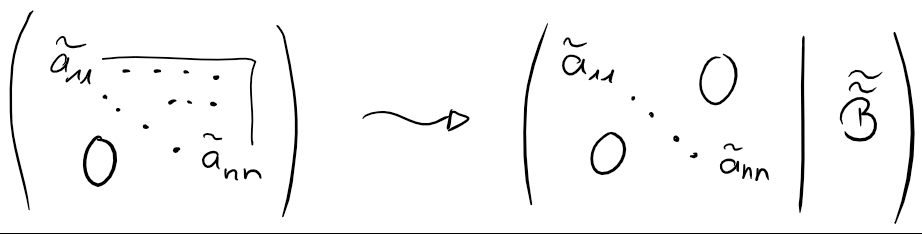
\includegraphics{Matrix_2} 
\item[iv)] Dann erhält man $A^{-1}$ indem man die i-te Zeile von $\tilde{ \tilde{B}}$ mit $\tilde{a_{ii}^{-1}}$ multipliziert:\\
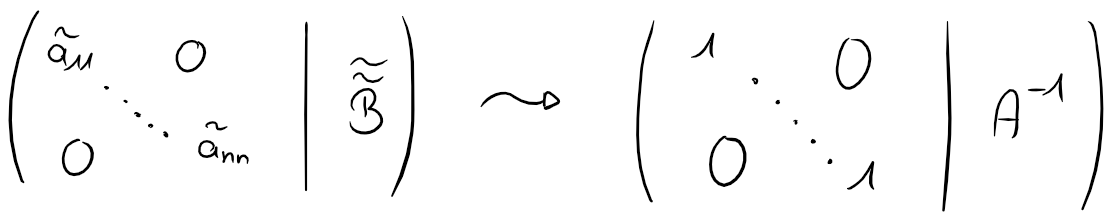
\includegraphics{Matrix_3}\\
Fazit:$(A|E_n)\underbrace{\rightsquigarrow}_{\text{elementare Zeilenumformung}}(E_n|A^{-1})$
\end{description}
\section{Beispiel}
Zu berechnen ist (im Fall der Existenz) $A^{-1}$ zur Matrix\[
A=\left(
\begin{array}{rrr}
0&1&-4\\
1&2&-1\\
1&1&2
\end{array}
\right)
\]
\[
\left(
\begin{array}{rrr|rrr}
0&1&-4&1&0&0\\
1&2&-1&0&1&0\\
1&1&2&0&0&1
\end{array}
\right)
\]
\[
\rightsquigarrow
\]
\[
\left(
\begin{array}{rrr|rrr}
1&2&-1&0&1&0\\
0&1&-4&1&0&0\\
1&1&2&0&0&1
\end{array}
\right)
\]\[
\rightsquigarrow
\]
\[
\left(
\begin{array}{rrr|rrr}
1&2&-1&0&1&0\\
0&1&-4&1&0&0\\
0&-1&3&0&-1&1
\end{array}
\right)
\]
\[
\rightsquigarrow
\]
\[
\left(
\begin{array}{rrr|rrr}
1&2&-1&0&1&0\\
0&1&-4&1&0&0\\
0&0&-1&1&-1&1
\end{array}
\right)
\]
\[
\rightsquigarrow
\]
\[
\left(
\begin{array}{rrr|rrr}
1&2&0&-1&2&-1\\
0&1&0&-3&4&-4\\
0&0&-1&1&-1&1
\end{array}
\right)
\]
\[
\rightsquigarrow
\]
\[
\left(
\begin{array}{rrr|rrr}
1&0&0&5&-6&7\\
0&1&0&-3&4&-4\\
0&0&-1&1&-1&1
\end{array}
\right)
\]
Also: \[A^{-1} = 
\left(
\begin{array}{rrr}
5&-6&7\\
-3&4&-4\\
-1&1&-1
\end{array}
\right)\]
\section{Bemerkung}
Üblicherweise betrachtet man drei Typen von elementaren Zeilenumformungen einer Matrix $A \in K^{m\times n}$:
\begin{description}
\item[Typ I:] Multiplikation einer Zeile mit $\lambda \in K\backslash\{0\}$
\item[Typ II:] Addition des $\lambda$-fachen der i-ten Zeile zur j-ten Zeile ($i\neq j, \lambda\in K\backslash\{0\}$)
\item[Typ III:] Vertauschen der i-ten und j-ten Zeile ($i \neq j$)
\end{description}
Das Verfahren zur Invertierung von Matrizen zeigt:\\
Jede Matrix $A\in GL(n,K)$ kann durch endlich viele elementare Zeilenumformungen von Typ I-III in die n-reihige Einheitsmatrix $E_n$ überführt werden.
\section{Bemerkung}
Ist $A\in GL(n,K)$ und ist $A^{-1}$ bereits berechnet, so kann für jede rechte Seite $b\in K^n$ die eindeutige Lösung $x$ zu $A*x=b$ durch Matrixmultiplikation berechnet werden:
\[x=(A^{-1}*A)x=A^{-1}(Ax)=(A^{-1}b)\]
\chapter{Lineare Abbildungen}
\section{Definition}
Eine Abbildung $F:V \rightarrow W$ zwischen $K-VR$ $V$ und $W$ wird \textbf{linear} oder (Vektorraum-) \textbf{Homomorphismus} genannt, falls \begin{description}
\item[i)] $\forall v\in V, \lambda \in K: F(\lambda v) = \lambda *F(v)$
\item[ii)] $\forall v_1,v_2 \in V: F(v_1+v_2)=F(v_1)+F(v_2)$
\end{description}
Ist $F$ bijektiv, so wird $F$ ein \textbf{Isomorphismus} genannt.
\section{Beispiel}
\begin{description}
\item[i)] Ist $A \in K^{m \times n}$, so ist $F_A:\mathbb{R}^n \rightarrow \mathbb{R}^m, x \mapsto A*x$ linear. Es gilt: $F_A(e_j) = A*e_j = \left(
\begin{array}{c}
a_{1j}\\
\vdots\\
a_{mj}
\end{array}
\right), j=1,...,n$, d.h.\\\textbf{die Spalten von $A$ sind die Bilder der Einheitsvektoren unter $F_A$.}\\
Falls $m=n$, so folgt leicht aus Satz 4.13:\\$F_A$ bijektiv $\Leftrightarrow$ $F_A$ injektiv $\Leftrightarrow$ $F_A$ surjektiv.
\item[ii)] Sei $[a,b] \subset \mathbb{R}$ ein Intervall $(-\infty <a<b<\infty)$. Dann sind:
\begin{description}
\item[I:] $C ([a,b]) \rightarrow C^1 ([a,b]):f \mapsto (x\mapsto \int_a^x f(y) dy)$
\item[D:] $C^1([a,b]) \rightarrow C([a,b]): f\mapsto f'$
\end{description}
linear. Nach dem Hauptsatz der Differential- und Integralrechnung gilt:
$D\circ I = id_{C([a,b])}$, sodass $I$ injektiv und D surjektiv ist. Da für konstante Funktionen $g\neq 0$ gilt: $(I\circ D)(g)=0$ sind weder I noch D Isomorphismen.
\end{description}
\section{Beispiel}
Ein Datenblock bestehend aus n Bits soll übertragen werden. Zur Fehlererkennung bei der Datenübertragung wird bei der Paritätsprüfung ein weiteres Bit, das sogenannte Paritätsbit an den Datenblock angehängt (vor der Datenübertragung). Es ist:
\begin{description}
\item[1], falls der Datenblock eine gerade Zahl von Einsen hat,
\item[0], sonst.
\end{description}
Dieses Vorgehen führt zu einer linearen Abbildung:
\[F: \mathbb{F}_2^n\rightarrow \mathbb{F}_2^{n+1}: x = \left(\begin{array}{c}
x_1\\\vdots\\x_n
\end{array}\right) \mapsto\left(
\begin{array}{c}
x_1\\\vdots\\x_n\\x_1+x_2+...+x_n
\end{array}
\right)\]
Dann hat $F(x)$ stets eine gerade Zahl von Einsen, sodass auf jeden Fall ein Übertragungsfehler vorliegt, wenn der empfangene Datenblock eine ungerade Zahl von Einsen hat.\\ In Matrixschreibweise gilt: $F=F_A$ mit $A=\left(
\begin{array}{ccc}
&E_n\\
1&\cdots&1
\end{array}
\right)$
\section{sehr einfacher Satz}
Sei $F:V \rightarrow W$ linear. Dann:
\begin{description}
\item[i)] $F(0) = 0$
\item[ii)] $F(\sum^n_{i=1} \lambda_i v_i) = \sum^n_{i=1}\lambda_iF(v_i)$ $(\lambda_1,...,\lambda_n \in K, v_1,...,v_n \in V)$
\item[iii)] Sind $V' \subset V, W'\subset W$ UVR, so sind $F(V') \subset W$ und $F^{-1}(W')\subset V$ UVR.
\item[iv)] Ist $(v_i)_{i\in I}$ linear abhängig in $V$, so ist $(F(v_i))_{i\in I}$ linear abhängig in $W$.
\item[v)] Ist $F$ ein Isomorphismus, so ist $F^{-1}$ linear.
\item[vi)] Ist $G: W \rightarrow U$ linear, so ist $G \circ F$ linear.
\end{description}
\subsection*{Beweis}
\textbf{i)-iv),vi) sind eine gute Übung.}
\begin{description}
\item[v)] Seien $w,w' \in W, \lambda,\mu \in K$. Seien $v:= F^{-1}(w), v' := F^{-1}(w')$. Dann: $\lambda w+ \mu w' = \lambda F(v) + \mu F(v') = F(\lambda v + \mu v')$\\
Anwenden der Umkehrfunktion liefert:\\
$F^{-1}(\lambda w + \mu w') = \lambda v + \mu v' = \lambda F^{-1}(w)+ \mu F^{-1}(w') \square$
\end{description}
\section{Definition (Endomorphismus und Automorphismus)}
Ist $F:V \rightarrow V$ linear, so wird $F$ ein \textbf{Endomorphismus} genannt. Bijektive Endomorphismen heißen \textbf{Automorphismen}.
\section{Folgerung}
Sei $V$ ein K-VR und $Aut(V)$ die Menge alle Automorphismen auf dem V. Dann wird $Aut(V)$ mit der Hintereinanderausführung zu einer Gruppe.
\section{Definition (Bild, Kern, Rang und Defekt)}
Sei $F:V\rightarrow W$ linear. Dann heißt $Im(F) := F(V)$ das \textbf{Bild} von $F$ und $Ker(F) := F^{-1}(\{0\})$ der \textbf{Kern} von $F$.\\
Beides sind UVR nach Satz 5.4. Man nennt $dim(Im(F))$ den \textbf{Rang} von $F$ und $dim(Ker(F))$ den \textbf{Defekt} von $F$.
\section{Satz}
Sei $F:V\rightarrow W $ linear. Dann:
\[F \text{ ist injektiv} \Leftrightarrow Ker(F) = \{0\}\] In diesem Fall gilt: Ist $(v_i)_{i\in I}$ linear unabhängig in $V$, so ist $(F(v_i))_{i\in I}$ linear unabhängig in $W$.
\subsection*{Beweis}
\begin{description}
\item["`$\Rightarrow$"'] klar
\item["`$\Leftarrow$"'] Seien $v,v' \in V$ mit $F(v) = F(v')$. Dann $F(v-v')=0$, d.h. $v-v' \in Ker(F)$. Somit: $v=v'$.
\end{description}
\subsection*{Zusatz:} Sei F injektiv und $(v_i)_{i\in I}$ linear unabhängig. Falls für eine Linearkombination \[\sum^n_{j=1} \lambda_j F(v_{i_j})=0,\] so \[F(\sum^n_{j=1} \lambda_j v_{i_j}) =0\] Also: \[\sum^n_{j=1}\lambda_j v_{i_j} = 0,\] da $Ker(F) = \{0\}$. Somit $\lambda_j=0$ für alle $j=1,...,n$, da $(v_i)_{i\in I}$ linear unabhängig. $\square$
\section{Satz} Sei $F:V\rightarrow W$ linear und $dim(v) < \infty$. Sind dann Basen $(v_1,...,v_k)$ von $Ker(F)$ und $(w_1,...,w_r)$ im $Im(F)$ gegeben. Ferner seien $u_1 \in F^{-1}(\{w_1\}),...,u_r\in F^{-1}(\{w_r\}$. Dann ist\[A = (u_1,...,u_r,v_1,...,v_k)\] eine Basis von V. Insbesondere:\[ dim(V) = dim(Im(F))+dim(Ker(F)) \text{ \textbf{(Dimensionsformel)}}\]
\subsection*{Beweis} Für $v \in V$ seinen $\mu_1,...,\mu_r\in K$ gegeben mit\[F(v)=\mu_1 w_1+...+ \mu_r w_r.\] Sei $v' := \mu_1 u_1 +...+ \mu_r u_r$. Da $F(v') = F(v)$, folgt: $v-v' \in Ker(F)$\\Also: $v-v' = \lambda_1v_1+...+\lambda_kv_k $ $(\lambda_1,...,\lambda_k \in K)$.\\Zusammen: $v=(v-v')+v' = \lambda_1v_1+...+\lambda_kv_k+\mu_1u_1+...+\mu_ru_r$.\\Also ist $A$ erzeugend.\\
Ist $\mu_1u_1+...+\mu_ru_r+\lambda_1v_1+...+\lambda_kv_k = 0$ für $\mu_1,...,\mu_r,\lambda_1,...,\lambda_k \in K$, so folgt durch Anwenden von $F$: $\mu_1w_1+...+\mu_rw_r =0$.\\ Da $(w_1,...,w_r)$ linear unabhängig, folgt $\mu_1=\mu_2=...=\mu_r = 0$.\\Also: $\lambda_1v_1+...+\lambda_kv_k=0$.\\Da $(v_1,...,v_k)$ linear unabhängig, folgt: $\lambda_1=...=\lambda_k=0$. Also ist $A$ linear unabhängig.$_\square$
\section{Folgerung}
Seien $V$ und $W$ endlich-dimensionale K-VR und $F:V\rightarrow W$ ein Isomorphismus. Dann: \[dim(V) = dim(W)\].
\subsection*{Anwendung auf lineare Gleichungssysteme:}
Sei $A \in K^{m\times n}$. Wir betrachten das sogenannte \textbf{homogene Problem}\[Ax=0 \in K^m.\] Da Lös$(A,0) = Ker(F_A)$, ist Lös$(A,0)$ ein UVR des $\mathbb{R}^n$.\\\\
Sei $\Phi_{A,0}$ die Abbildung aus Algorithmus 1.8. Induktiv überzeugt man sich, dass $c_{ik} \in K$ existieren, sodass mit $r:=$Zeilenrang$(\tilde{A})$\[x_i(\lambda) = \dfrac{1}{\tilde{a}_{ii}}(-\sum^n_{j=i+1}\tilde{a}_{ij}x_j(\lambda))= \sum^{n-r}_{k=1} c_{ik}\lambda_k\]
Also ist $\Phi_{A,0}:\mathbb{R}^{n-r} \rightarrow \text{Lös}(A,0)$ in Algorithmus 1.8 linear und nach dem dort Gezeigten bijektiv. Folgerung 5.10 impliziert:\[dim(\text{Lös}(A,0))=n-\text{Zeilenrang}(A)\]
Andererseits impliziert die Dimensionsformel \[n=\text{Rang}(F_A)+dim(\text{Lös}(A,0))\]
Da für alle $\lambda_1,...,\lambda_n\in K$ gilt:\[ F_A(\sum^n_{j=1}\lambda_je_j)= \sum^n_{j=1}\lambda_j A*e_j=\sum^n_{j=1}\lambda_j \left(
\begin{array}{c}
a_{1j}\\ \vdots \\ a_{mj}
\end{array}
\right),
\] folgt: Das Bild von $F_A$ ist der Spaltenraum von $A$.\\\\
Zusammen ergibt sich:
\section{Satz}
Sei $A\in K^{m \times n}$. Dann:
\[\text{Rang}(F_A) = \text{Spaltenrang}(A)= \text{Zeilenrang}(A)\]
und Lös$(A,0)$ ist ein UVR des $\mathbb{R}^n$ der Dimension $n-\text{Rang}(F_A)$\\\\
Wir betrachten nun das \textbf{inhomogene Problem} $Ax=b,\ b\in K^m\backslash\{0\}$.
\section{Lemma} Sei $x \in $ Lös$(A,b)$. Dann:\[y\in \text{Lös}(A,b) \Leftrightarrow \exists z \in \text{Lös}(A,0): y = x+z\]
\subsection*{Beweis}
\begin{description}
\item["`$\Rightarrow$"'] $A(x-y) = Ax-Ay = b-b = 0$
\item["`$\Leftarrow$"'] $Ay=A(x+z) = Ax+Az = b+0 = b$ $\square$
\end{description}
\section{Definition (affiner Unterraum)} Sei $U$ ein UVR eines K-VR $V$ und $v \in V$. Eine Menge der Form\[v+U:=\left\{v+u|u\in U\right\}\] wird eine \textbf{affiner Unterraum} von $V$ genannt.
\section{Bemerkung}
Ist $v+U = v'+U'$, so gilt $U=U'$ und $v' \in v+U$. Insbesondere ist $dim(v+U) := dim(U)$ wohldefiniert.
\section{Satz}Seien $A\in K^{m \times n}$ und $b \in K^m\backslash \{0\}$. Dann ist Lös$(A,b)$ entweder leer oder ein affiner Unterraum der Dimension $n-\text{Rang}(F_A)$, nämlich\[\text{Lös}(A,b)=x+\text{Lös}(A,0),\] wobei $x\in \text{Lös}(A,b)$ beliebig.
\subsection*{Beweis} Lemma 5.12 und Satz 5.11. $\square$
\section{Bemerkung}
Die Gesamtheit der Lösung des inhomogenen Problems findet man, indem man zunächst eine Lösung zu $Ax=b$ bestimmt (spezielle Lösung) und dann alle Lösungen des homogenen Problems bestimmt.
\section{Beispiel}
Sei $a\in K^n \backslash \{0\}$ und $b\in K$. Eine Menge der Form\[H(a,b)=\left\{x\in K^n|a^T*x=b\right\}\] wird \textbf{Hyperebene} genannt.\\
Da Rang$(F_{a^T}) = 1$, ist $H(a,b)$ ein affiner Unterraum der Dimension $n-1$ im $K^n$.\\Ist $K^n=\mathbb{R}^3$, so sind die Hyperebenen gerade die Ebenen im "`üblichen"' Sinn.
\chapter{Koordinatentransformationen}
\section{Satz (Koordinatensystem)}
Sei $V$ ein K-VR mit Basis $B=(v_1,...,v_n)$. Dann existiert genau ein Isomorphismus $\Phi_B:K^n \rightarrow V$ mit $\Phi_B(e_j)=v_j$ für $j=1,...,n$. Man nennt $\Phi_B$ das durch $B$ bestimmte \textbf{Koordinatensystem} in $V$ und $\Phi^{-1}_B(v)$ die \textbf{Koordinaten} von $v$.
\subsection*{Beweis}
Sei $x=\left(\begin{array}{c}
x_1\\\vdots\\x_n
\end{array}\right) \in K^n$. Dann impliziert die Linearität:\[\Phi_B(x) = \Phi_B(\sum^n_{j=1}x_je_j)=\sum^n_{j=1}x_j \Phi_B(e_j) = \sum^n_{j=1} x_j v_j\] Also ist $\Phi_B$ eindeutig bestimmt.\\
Da $(v_1,...,v_n)$ eine Basis von V ist, existiert zu jedem $v\in V$ genau ein $x =\left( \begin{array}{c}
x_1\\\vdots\\x_n
\end{array}\right) \in K^n$ mit $v = \sum^n_{j=1}x_jv_j = \Phi_B(x)$. Also ist $\Phi_B$ bijektiv. $\square$
\section{Bemerkung}
Zwei K-VR $U$ und $V$ werden \textbf{isomorph} genannt, falls ein Isomorphismus $F:U\rightarrow V$ existiert.\\\\
Satz 6.1 und Folgerung 5.10 zeigen: Zwei endlichdimensionale K-VR sind isomorph genau dann, wenn sie die gleiche Dimension haben.
\section{Beispiel (Diskrete Kosinustransformation zur Datenkomprimierung)}
Ein Vektor $v\in \mathbb{R}^n$ soll in komprimierter Form gespeichert werden.\\Eine Möglichkeit: Transformation in den Frequenzbereich. Dazu sei\[
v_k:= \left(
\begin{array}{c}
cos\left(\frac{0,5}{n}(k-1)\pi\right)\\
cos\left(\frac{1,5}{n}(k-1)\pi\right)\\
\vdots\\
cos\left((1-\frac{0,5}{n})(k-1)\pi\right)\\
\end{array}
\right)
\]
Man kann zeigen, dass $B = (v_1,...,v_n)$ eine Basis des $\mathbb{R}^n$ bilden. Sie besteht aus Kosinusschwingungen zu unterschiedlichen Frequenzen, die an den Punkten $\frac{j+0,5}{n}$ abgetastet werden. Seien $x= \left(
\begin{array}{c}
x_1\\\vdots\\x_n
\end{array}
\right)$ die Koordinaten von $v\in \mathbb{R}^n$ im durch $B$ bestimmten Koordinatensystem, das heißt $v=\sum^n_{k=1}x_kv_k$. In einem Quantisierungsschritt setzt man für ein vorgegebenes $\sigma>0$:
\[
\tilde{x}_k=\left\{\begin{array}{cc}
x_k&,|x_k|\geq \sigma\\
0&,|x_k|<\sigma
\end{array}\right.
\] und speichert nur $\tilde{x}_1,...,\tilde{x}_{i_{max}}$, wobei $i_{max}$ der größte Index ist, für den $\tilde{x}_{i_{max}} \neq 0$. Die Rekonstruktion
\[
\tilde{v} = \sum^{i_{max}}_{k=1} \tilde{x}_k v_k
\]
ist besser, je kleiner $\sigma$ ist. Die Einsparung bei Speicherplatz ist höher, je größer $\sigma$ ist.\\Ein ähnliches Verfahren für Matrizen statt Vektoren kommt bei JPEG zum Einsatz.
\section{Bemerkung}
Sei $B=(b_1,...,b_n)$ eine Basis im $K^n$. Dann hat das Koordinatensystem $\Phi_B$ die Darstellung:\[\Phi_B(x) = T_B*x\] wobei die Vektoren $b_1,...,b_n$ die Spalten von $T_B \in K^{n \times n}$ sind. Die Matrix $T_B$ ist dann invertierbar nach Satz 4.13 und es gilt:\[\Phi^{-1}_B(v) = T^{-1}_B*v,\ v\in K^n.\]
Man erhält also die Koordinaten durch Multiplikation mit $T^{-1}_B$.
\section{sehr einfaches Beispiel}
Sei $b_1=\left(
\begin{array}{c}
2\\1
\end{array}
\right), b_2 = \left(
\begin{array}{c}
1\\3
\end{array}
\right)$. Dann ist $B=(b_1,b_2)$ eine Basis im $\mathbb{R}^2$. Mit dem Verfahren zu Matrixinvertierung aus Kapitel 4 berechnet man leicht:\[
T^{-1}_B = \left(
\begin{array}{cc}
\frac{3}{5}&-\frac{1}{5}\\
-\frac{1}{5}&\frac{2}{5}
\end{array}
\right)
\] Also gilt für jeden Vektor $v=\left(
\begin{array}{c}
v_1\\v_2
\end{array}
\right)\in \mathbb{R}^2$:
\[v=\left(\frac{3}{5}v_1 - \frac{1}{5}v_2\right)*b_1+\left(-\frac{1}{5}v_1+\frac{2}{5}v_2\right)*b_2\]
\section{Satz}
Gegeben sei K-VRe $V$ mit Basis $\mathscr{A} = (v_1,...,v_n)$ und $W$ mit Basis $\mathscr{B} = (w_1,...,w_m)$. Dann gibt es zu jeder linearen Abbildung $F:V\rightarrow W$ genau eine Matrix $M_\mathscr{B}^\mathscr{A}(F) = (a_{ij})\in K^{m\times n}$ mit \[F(v_j)= \sum ^m_{i=1} a_{ij}w_i,j=1,...,n \ (*)\]
Ferner gilt:
\[(\Phi_B^{-1} \circ F \circ \Phi_A)(x) = M^\mathscr{A}_\mathscr{B}(F)*x, x\in K^n \ (**)\]
Man nennt $M^\mathscr{A}_\mathscr{B}(F)$ die \textbf{darstellende Matrix} von $F$ bzgl. $A$ und $B$.
\subsection*{Beweis}
Da $B$ eine Basis von $W$ ist, sind die Spalten von $M^\mathscr{A}_\mathscr{B}(F)$ durch $(*)$ eindeutig bestimmt. Aufgrund der Linearität reicht es, $(**)$ auf den kanonischen Einheitsvektor zu prüfen. Es gilt:\[(\Phi^{-1}_\mathscr{B}\circ F\circ \Phi_\mathscr{A})(e_j)=\Phi_\mathscr{B}^{-1}(F(v_j))=\Phi_\mathscr{B}^{-1}(\sum^m_{i=1}a_{ij}w_i)\]\[=\sum^m_{i=1}a_{ij}\Phi_\mathscr{B}^{-1}(w_i) = \sum^m_{i=1}a_{ij}e_i\]
\[= \left(
\begin{array}{c}
a_{1j}\\a_{2j}\\\vdots\\a_{mj}
\end{array}
\right) = M_\mathscr{B}^\mathscr{A}(F)*e_j.\square\]
\subsection*{Frage:}
Wie wählt man die Basen $\mathscr{A},\mathscr{B}$ so, dass die darstellende Matrix besonders "`einfach"' ist?
\section{Satz} Sei $F:V\rightarrow W$ linear, dann $dim(V)=n$, $dim(W)=m$ und $r$ der Rang von $F$. Dann gibt es Basen $\mathscr{A}$ von $V$ und $\mathscr{B}$ von $W$, sodass \[
M^\mathscr{A}_\mathscr{B}(F)= \left(
\begin{array}{cc}
E_r&0\\
0&0
\end{array}
\right)
\]
\subsection*{Beweis:}
Eine Basis $(w_1,...,w_r)$ von $Im(F)$ werde auf irgendeine Weise zu einer Basis $\mathscr{B}=(w_1,...,w_m)$ von $W$ ergänzt. Ferne seinen $v_i \in F^{-1}(\{w_i\})$ für $i=1,...,r$ und $(v_{r+1},...,v_n)$ eine Basis von $Ker(F)$. Nach Satz 5.9 ist $A=(v_1,...,v_n)$ eine Basis von $V$. Es gilt:\[
F(v_j)=\left\{
\begin{array}{ll}
w_j&,j=1,...,r\\
0&,j=r+1,...,n
\end{array}
\right.
\]
Also gilt $M^\mathscr{A}_\mathscr{B}(F)=(a_{ij})$ mit
\[
a_{ij}= \left\{
\begin{array}{ll}
1&, 0\leq i=j \leq r\\
0&, \text{ sonst}
\end{array}
\right. _\square
\]
\section{Bemerkung}
Seien $A,B\in K^{m\times n}$. Dann wird $A$ \textbf{äquivalent} zu $B$ genannt, falls $T\in \text{GL}(n,K),S\in \text{GL}(m,K)$ existieren mit \[B=S*A*T^{-1}.\]Wendet man Satz 6.7 auf $F_A:\mathbb{R}^n \rightarrow \mathbb{R}^m$ an und setzt man $T=T^{-1}_\mathscr{A}, S=T^{-1}_\mathscr{B}$ so gilt mit Satz 6.6 und Bemerkung 6.4:\[SAT^{-1}=T^{-1}_\mathscr{B}AT^{-1}_\mathscr{A} = M^{\mathscr{A}}_{\mathscr{B}}(F_A)=
\left(
\begin{array}{cc}
E_r&0\\
0&0
\end{array}
\right),\]
wobei $r$ der Rang von $A$ ist. Also ist $A$ äquivalent zu $\left(\begin{array}{cc}
E_r&0\\
0&0
\end{array}\right)$.
Man nennt dies die Normalform von $A$(bzgl. Äquivalenz).
\section{Beispiel}
Sei $A=\left(
\begin{array}{cc}
1&2\\
2&2\\
0&1\\
\end{array}
\right)$. Gesucht sind Basen $\mathscr{A}$ im $\mathbb{R}^2$ und $\mathscr{B}$ im $\mathbb{R}^3$, sodass $M_\mathscr{B}^\mathscr{A}(F_A)$ Normalform (also die Form aus Satz 6.7) hat.\\
Da $Im(F_A) = ZR(A^T)$, kann man mit Algorithmus 4.2 eine Basis von $Im(F_A)$ berechnen.
\[A^T=\left(
\begin{array}{ccc}
1&2&0\\
2&2&1
\end{array}
\right)\rightsquigarrow \left(
\begin{array}{ccc}
1&2&0\\
0&-2&1
\end{array}
\right)\]
Also ist $\left(\left( \begin{array}{c}
1\\2\\0
\end{array}\right),\left(\begin{array}{c}
0\\-2\\1
\end{array}
\right)\right)$ eine Basis vom $Im(F_A)$\\Diese ergänzen wir zu einer Basis des $\mathbb{R}^3$
\[\mathscr{B}=\left(\left(\begin{array}{c}
1\\2\\0
\end{array}\right),\left(\begin{array}{c}
0\\-2\\1
\end{array}\right),\left(\begin{array}{c}
0\\0\\1
\end{array}\right)\right)
\]
Da Rang$(F_A) = 2$, ist $Ker(F_A) = \{0\}$. Die Basis $\mathscr{A}$ im $\mathbb{R}^2$ besteht also aus Lösungen $v_1,v_2$ zu $A*v_1\left(
\begin{array}{c}
1\\2\\0
\end{array}
\right),A*v_2=\left(\begin{array}{c}
0\\-2\\1
\end{array}
\right)$\\
Der Gaußalgorithmus liefert:\[
\left(
\begin{array}{cc|cc}
1&2&1&0\\
2&2&2&-2\\
0&1&0&1
\end{array}
\right)\rightsquigarrow
\left(
\begin{array}{cc|cc}
1&2&1&0\\
0&-2&0&-2\\
0&1&0&1
\end{array}
\right)\rightsquigarrow
\left(
\begin{array}{cc|cc}
1&2&1&0\\
0&-2&0&-2\\
0&0&0&0
\end{array}
\right)
\]
Also: $\mathscr{A}=\left(\left(\begin{array}{c}
1\\0
\end{array}
\right),\left(\begin{array}{c}
2\\1
\end{array}
\right)\right)$
\chapter{Eigenwertproblem}
\section*{Frage:}
Sei $V$ ein $n$-dim K-VR und $F:V\rightarrow V$ ein Endomorphismus. Wie findet man eine Basis $\mathscr{B}$ von $V$, sodass $M^\mathscr{B}_\mathscr{B}(F)$ eine "`möglichst einfache "' Darstellung hat?\\
Diese (schwierige) Frage führt zu:
\section{Definition}
Sei $F:V\rightarrow V$ ein Endomorphismus. $\lambda \in K$ wird \textbf{Eigenwert} zu F genannt, falls ein $v\in V \backslash \{0\}$ existiert mit \[F(v)=\lambda*v\]Jedes solche $v$ wird ein \textbf{Eigenvektor} von F zum Eigenwert $\lambda$ genannt.\\
Mit $\text{Eig}(F,\lambda):=\{v\in V|F(v) = \lambda v\} = \text{Ker}(F-\lambda \text{ id}_v)$ bezeichnen wir den \textbf{Eigenraum} von $F$ zu $\lambda \in K$. Hier ist $\text{id}_v:V\rightarrow V, v \mapsto v$.
\section{Bemerkung}
$\lambda$ Eigenwert zu $F \Leftrightarrow$ $\text{Eig}(F,\lambda) \neq \{0\}$. In diesem Fall ist Eig$(F,\lambda)\backslash \{0\}$ die Menge aller Eigenvektoren zum Eigenwert $\lambda$.
\section{Definition}
Ein Endomorphismus $F:V\rightarrow V$ wird \textbf{diagonalisierbar} genannt, falls eine Basis $\mathscr{B} = (v_1,...,v_n)$ und $\lambda_1,...,\lambda_n \in K$ existieren mit $M^\mathscr{B}_\mathscr{B}(F)=\left(\begin{array}{cccc}
\lambda_1&0&\cdots&0\\
0&\ddots&&\vdots\\
\vdots&&\ddots&0\\
0&\cdots&0&\lambda_n
\end{array}
\right)$
\section{Satz}
Sei $V$ ein n-dim K-VR und $F:V \rightarrow V$ linear. Dann:\[F\text{ ist diagonalisierbar} \Leftrightarrow \text{Es ex. eine Basis aus Eigenvektoren zu } F \text{ in } V\]
\subsection*{Beweis}
Sei $F$ diagonalisierbar und für eine Basis $\mathscr{B}=(v_1,...,v_n)$ und $\lambda_1,...,\lambda_n \in K$ gelte: $M^\mathscr{B}_\mathscr{B}(F)=\left(\begin{array}{cccc}
\lambda_1&0&\cdots&0\\
0&\ddots&&\vdots\\
\vdots&&\ddots&0\\
0&\cdots&0&\lambda_n
\end{array}
\right)$\\
Dann:\\
$F(v_j) = F(\Phi_\mathscr{B} (e_j)) = \Phi_\mathscr{B}\underbrace{(M^\mathscr{B}_\mathscr{B}(F)*e_j)}_{=\lambda_je_j} = \lambda_j\Phi_\mathscr{B}(e_j)=\lambda_jv_j$\\
Also ist $v_j$ ein Eigenvektor zum Eigenwert $\lambda_j$.\\
Ist andererseits $\mathscr{B}=(v_1,...,v_n)$ eine Basis mit Eigenvektoren zu (nicht notwendigerweise verschiedenen) Eigenwerten $\lambda_1,...,\lambda_n$.\\Dann:\\
$M^\mathscr{B}_\mathscr{B}(F)*e_j=(\Phi_\mathscr{B}^{-1} \circ F \circ \Phi_\mathscr{B})(e_j) = \Phi_\mathscr{B}^{-1} ((\underbrace{F(v_j)}_{\lambda_jv_j})=\lambda_j \Phi_\mathscr{B}^{-1}(v_j) = \lambda_je_j$.\\
Also hat $M^\mathscr{B}_\mathscr{B}(F)$ Diagonalform. $_\square$
\section{Beispiel}
Für $\alpha \in \{-1,0,1\}$ sei $A=\left( \begin{array}{cc}
0&\alpha\\
1&0
\end{array}\right)$.\\
Frage: Ist $F_A: \mathbb{R}^2 \rightarrow \mathbb{R}^2, x \mapsto Ax$ diagonalisierbar?\\$\lambda$ ist Eigenwert zu $F_A$ $\Leftrightarrow$ Lös$(A-\lambda E_2,0)\neq \{0\}$\\
Mit dem Gauß-Algorithmus berechnen wir:\[\left(
\begin{array}{cc|c}
-\lambda &\alpha &0\\
1& -\lambda &0
\end{array}\right) \rightsquigarrow \left(\begin{array}{cc|c}
1 & -\lambda &0\\
-\lambda &\alpha &0
\end{array} \right)\rightsquigarrow\left(\begin{array}{cc|c}
1 &-\lambda &0\\
0& -\lambda^2+\alpha &0
\end{array}\right)
\]
Also: Lös$(A-\lambda E_2,0)\neq \{0\} \Leftrightarrow \lambda^2 = \alpha$.
\begin{itemize}
\item $\alpha = 1$:  $\lambda_1 = 1$ und $\lambda_2 = -1$ sind Eigenwerte mit Eigenvektoren $v_1=\left(\begin{array}{c}
1\\1
\end{array}
\right),v_2=\left(\begin{array}{c}
1\\-1
\end{array}
\right)$.\\Mit $\mathscr{B} = \left(\left(\begin{array}{c}
1\\1
\end{array}
\right),\left(\begin{array}{c}
1\\-1
\end{array}
\right)\right)$ folgt: $M^\mathscr{B}_\mathscr{B}(F_A) = \left(
\begin{array}{cc}
1&0\\
0&-1
\end{array}
\right)$
\item $\alpha = -1$: $\lambda^2 = -1$ hat keine Lösung in $\mathbb{R}$. Also ist $F_A: \mathbb{R}^2 \rightarrow \mathbb{R}^2$ nicht diagonalisierbar. Wir betrachten: $F_A:\mathbb{C}^2 \rightarrow \mathbb{C}^2$. Dann lösen $\lambda_1 = i$ und $\lambda_2 = -i$ die Gleichung $\lambda^2 =-1$. Zugehörige Eigenvektoren sind: $v_1 = \left(
\begin{array}{c}
i\\1
\end{array}
\right)$ und $v_2 = \left(
\begin{array}{c}
-i\\1
\end{array}
\right)$. Also folgt mit $\mathscr{B} =\left(\left(
\begin{array}{c}
i\\1
\end{array}
\right), \left(
\begin{array}{c}
-i\\1
\end{array}
\right)\right) $, dass $M^\mathscr{B}_\mathscr{B}(F_A)= \left(
\begin{array}{cc}
i&0\\
0&-i
\end{array}
\right)$. Also ist $F_A$ über $\mathbb{C}$ diagonalisierbar.
\item $\alpha = 0$: Hier ist $\lambda = 0$ einziger Eigenwert und Eig$(F_A,0)= \text{span}(e_2)$ hat Dimension 1. Also existiert weder über $\mathbb{R}$ noch über $\mathbb{C}$ eine Basis aus Eigenvektoren, das heißt $F_A$ ist nicht diagonalisierbar.
\end{itemize}
\section{Bemerkung}
Eigenwerte kann man als Nullstellen des sog. charachteristischen Polynoms finden. Dazu später mehr.
\section{Satz}
Sei $F:V \rightarrow V$ linear und seien $v_1,...,v_n$ Eigenvektoren zu paarweise verschiedenen Eigenwerten $\lambda_1,...,\lambda_n$. Dann ist $(v_1,...,v_n)$ linear unabhängig. Insbesondere gilt: $n \leq dim(V)$.
\subsection*{Beweis}
Induktion über n:
\begin{description}
\item[n=1:] klar, da $v_1\neq 0$
\item[n-1 $\rightsquigarrow$ n:] Sei \[\alpha_1 v_1+ \alpha_2 v_2 +...+ \alpha_n v_n = 0\] für $\alpha_1,...,\alpha_n \in K$. Dann folgt durch Anwenden von $F$ bzw. Multiplikation $\lambda_n$: \[\alpha_1\lambda_1v_1+\alpha_2\lambda_2v_2...+\alpha_n\lambda_nv_n=0\]\[\alpha_1\lambda_nv_1+\alpha_2\lambda_nv_2...+\alpha_n\lambda_nv_n=0\]
Also:\[\alpha_1(\lambda_1-\lambda_n)v_1+\alpha_2(\lambda_2-\lambda_n)v_2+...+\alpha_{n-1}(\lambda_{n-1}-\lambda_n)v_{n-1}\]
Nach Induktionsannahme ist $(v_1,...,v_n-1)$ linear unabhängig. Da $\lambda_j \neq \lambda_n$ für alle $j=1,...,n-1$, folgt: $\alpha_1=\alpha_2=...=\alpha_{n-1} = 0$. Da $v_n \neq 0$ folgt $\alpha_n=0$. $\square$
\end{description}
\section{Folgerung}
$F: V\rightarrow V$ linear, habe n paarweise verschiedene Eigenwerte, wobei $n = dim (V)$. Dann ist $F$ diagonalisierbar.
\subsection*{Beweis}
Satz 7.7 und Satz 7.4. $_\square$
\section{Bemerkung}
\begin{description}
\item[i)] Ist $A\in K^{n\times n}$, so nennt man die Eigenwerte (bzw. -vektoren) von $F_A$ auch Eigenwerte (bzw. -vektoren) von $A$.
\item[ii)] $A,C \in K^{n \times n}$ heißen \textbf{ähnlich}, falls ein $B\in $GL$(n,K)$ existiert mit $A=BCB^{-1}$. $A$ wird diagonalisierbar genannt, falls $A$ ähnlich zu einer Diagonalmatrix \[C = \left(\begin{array}{cccc}
\lambda_1&0&\cdots&0\\
0&\ddots&&\vdots\\
\vdots&&\ddots&0\\
0&\cdots&0&\lambda_n
\end{array}\right)\] ist (oder anders formuliert, wenn $F_A$ diagonalisierbar ist).
\end{description}
\section{Satz}
Sei $A\in K^{n \times n}$ und $C$ sei ähnlich zu $A$. Dann haben $A,A^T,C$ die selben Eigenwerte.
\subsection*{Man beachte:}
$\lambda$ ist Eigenwert zu $A$ $\Leftrightarrow$ $A-\lambda E_n$ nicht invertierbar.
\subsection*{Beweis}
$A-\lambda E_n$ invertierbar $\Leftrightarrow$ $(A-\lambda E_n)^T$ invertierbar\\$\Leftrightarrow$ $A^T-(\lambda E_n)^T$ invertierbar\\$\Leftrightarrow$ $A^T - \lambda E_n$ invertierbar\\
\textbf{Also:} $\lambda$ Eigenwert zu $A$ $\Leftrightarrow$ $\lambda$ Eigenwert zu $A^T$.\\
Sei nun $A=BCB^{-1}$ für ein $B\in \text{GL}(n,k)$.\\
Dann:\\
$A-\lambda E_n = BCB^{-1} -\lambda E_n = BCB^{-1} - B\lambda E_n B^{-1} = B(C-\lambda E_n) B^{-1}$\\
Also:\\
$(A-\lambda E_n) v= 0 \Leftrightarrow (C-\lambda E_n)(B^{-1}v)=0$, d.h. $v$ ist Eigenvektor von $A$ zum Eigenwert $\lambda$ genau dann, wenn $B^{-1}v$ Eigenvektor von $C$ zum Eigenwert $\lambda$ ist. $\square$\\\\
Im Fall $K= \mathbb{C}$ kann man zeigen:
\section{Satz (Jordansche Normalform)}
Jede Matrix $A\in \mathbb{C}^{n \times n}$ ist ähnlich zu einer Matrix der Form:\\
$
\left(
\begin{array}{ccc}
J_1&&0\\
&\ddots&\\
0&&J_p
\end{array}
\right)
$\\
wobei jeder "`Jordanblock"' $J_i$ eine quadratische Matrix der Form\\
$J_i=\left(
\begin{array}{cccc}
\lambda_i &1 &&0\\
&\ddots&\ddots&\\
&&\ddots&1\\
0&&&\lambda_i
\end{array}
\right)$\\
ist, wobei $\lambda_i$ (nicht notwendigerweise verschiedene) Eigenwerte von A sind.
\chapter{Eigenwertprobleme für stochastische Matrizen}
\subsection*{Zurück zum Page-Rank-Beispiel 1.1:}
Gegeben seien n Internetseiten. Wir definieren Matrizen $L=(l_{ij})_{i,j=1,...,n},S=(s_{ij})_{i,j=1,...,n},\\G=(g_{ij})_{i,j=1,...,n}$ durch
\[l_{ij}=\left\{
\begin{array}{ll}
\dfrac{1}{c_j} &\text{, falls Seite j auf Seite i verlinkt}\\
c_j&\text{, sonst}
\end{array}\right.
\]\[
c_j = \text{Anzahl der Seiten, auf die j verlinkt.}
\]
\[a_j = \left\{
\begin{array}{ll}
1&\text{, Seite j verlinkt auf keine Seite}\\
0&\text{, sonst}
\end{array}
\right.\]
\[a=\left(\begin{array}{c}
a_1\\\vdots \\ a_n
\end{array}\right), e=\left(
\begin{array}{c}
1\\\vdots\\1
\end{array}
\right)\in \mathbb{R}^n\]
\[S:= L+\frac{1}{n}ea^T\]
\[G:= d*S+(1-d)\frac{1}{n}ee^T\]
für einen Damping-Faktor $0<d<1$.\\
Gleichungssystem aus Bsp: 1.1 $(*)$ ist dann gerade $(d*S -E_n) x = -\frac{1-d}{n}e$ (P)
\section{Lemma}
$x \in \mathbb{R}^n$ löst $(P)$ genau dann, wenn $x$ Eigenvektor von $G$ zum Eigenwert 1 ist und $\sum^n_{i=1}x_i=1$
\subsection*{Beweis:}
$x$ löse $(P)$. Dann:\[\sum^n_{i=1} x_i = e^Tx = e^T E_n x = e^T(d*S x+ \frac{1-d}{n}e)\]
\[=d*e^TS+\frac{1-d}{n}e^Te\]
Nun $e^Te = \sum^n_{i=1}1*1 = n$
\[e^TS = (\sigma_1,...,\sigma_n)\in \mathbb{R}^{1\times n},\] wobei \[\sigma_j = \sum^n_{i=1}1*s_{ij}\] die Summe der Einträge der j-ten Spalte von $S$ ist.\\Da
\[\sigma_j = \sum^n_{i=1} l_{ij}+a_j = 1,\] folgt: \[e^TS=e^T\] und also: \[\sum^n_{i=1}x_i = d(\sum^n_{i=1}x_i) + (1-d)\] Da $d \neq 1$ folgt:\[e^Tx = \sum^n_{i=1}x_i = 1\]
Aus $(P)$ folgt weiter:
\[Gx = d*Sx +(1-d) \frac{1}{n} e\underbrace{ e^Tx}_{=1} = E_n x = x\]
Also ist $x$ Eigenvektor von $G$ zum Eigenwert 1.\\
Sei nun $x$ Eigenvektor von $G$ zum Eigenwert 1 mit $\sum^n_{i=1}x_i = 1$. Dann:
\[(d*S-E_n)x =\underbrace{ Gx -x}_{=0} -(1-d) \frac{1}{n} e\underbrace{e^Tx}_{=1} = -\frac{1-d}{n}e\] Also löst $x$ $(P)$. $\square$
\section{Definition}
Eine Matrix $A\in \mathbb{R}^{n \times n}$ mit nicht negativen Einträgen (also $a_{ij} \geq 0 \text{ } \forall i,j = 1,...,n$) h heißt:
\begin{itemize}
\item \textbf{Zeilenstochastisch}, falls $A*e=e$
\item \textbf{Spaltenstochastisch}, falls $e^T A= e^T$\\
(Hier sind also im ersten Fall alle Zeilensummen = 1, im zweiten Fall alle Spaltensummen =1).
\end{itemize}
\section{Lemma}
$S$ und $G$ sind spaltenstochastisch.
\subsection*{Beweis:}
Die Nichtnegativität der Einträge ist klar. $e^TS=e^T$ wurde in Lemma 8.1 mitgezeigt.\\Also:
\[e^TG=de^TS+\frac{1-d}{n}\underbrace{e^Te}_{=n}e^T = d e^T+(1-d)e^T = e^T\]$\square$
\section{Satz}
$A\in \mathbb{R}^{n \times n}$ sei zeilen- oder spaltenstochastisch. Dann:
\begin{description}
\item[i)] 1 ist Eigenwert zu A.
\item[ii)] Betrachtet man $A$ als Element von $\mathbb{C}^{n\times n}$ und ist $\lambda \in \mathbb{C}$ Eigenwert von $A$, so: $|\lambda|\leq 1$.\\
Kurz: 1 ist der betragsgrößte Eigenwert zu A.\\\\
\textbf{Erinnerung:} Ist $z = a+ib \in \mathbb{C} (a,b\in \mathbb{R})$, so $|z| :=\sqrt{a^2+b^2}$
\end{description}
\subsection*{Beweis:}
Ohne Einschränkung sei $A$ zeilenstochastisch (Satz 7.10).
\begin{description}
\item[i)] Nach Def. 8.2 ist dann $e$ Eigenvektor von $A$ zum Eigenwert 1.
\item[ii)] Sei $v \in \mathbb{C}^n \backslash \{0\}$ ein Eigenvektor zum Eigenwert $\lambda \in \mathbb{C}$.\\
Dann gilt nach den Rechenregeln für den komplexen Betrag aus MfI 1:\[|\lambda|*max|v_i|_{i=1,...,n} = max(|\lambda||v_i|)_{i=1,...,n}\]
\[max|\lambda v_i| =_{Av=\lambda v} max|\sum^n_{j=1}a_{ij}v_j|\]
\[\leq max \sum^n_{j=1} \underbrace{a_{ij}}_{\geq 0}|v_j| \leq max _{k=1,...,n} |v_k| max _{i=1,...,n} \underbrace{\sum^n_{j=1}a_{ij}}_{1} = max_{k=1,...,n}|v_k|\]
Da $v \neq 0$, folgt $max_k|v_k| \neq 0$. Also $|\lambda|\leq 1$. $\square$
\end{description}
Das folgende als \textbf{Potenzmethode} oder \textbf{einfache Vektoriteration} bekannte Verfahren kann verwendet werden, um unter geeigneten Voraussetzungen einen Eigenvektor zum betragsgrößten Eigenwert einer Matrix $A\in \mathbb{C}^{n\times n}$ zu bestimmen:\\
Sei $\lambda$ der betragsgrößte Eigenwert von $v^{0} \in \mathbb{C}^n$ ein "`geeignet"' gewählter Startvektor. Setze:
\[v^{(k)} := Av^{(k-1)},k\in \mathbb{N}\]\[=A^kv^{(0)},a^k=\underbrace{A\cdots A}_{k-mal}\]
Dann gilt typischerweise:\\
Für alle $i=1,...,n$ konvergiert $(\lambda^{-k}v_i^{(k)})_{k\in \mathbb{N}}$ gegen ein $v_i \in \mathbb{C}$, wobei $v=\left(\begin{array}{c}
v_1\\\vdots\\v_n
\end{array}
\right)$ ein Eigenvektor zum Eigenwert $\lambda$ ist.\\
\textit{"`(s. Stoer/Bulirsch, Einführung in die Numerische Mathematik II, Springer)"'}\\
Für spaltenstochastische Matrizen gilt:
\section{Satz (Spezialfall des Satzes von Frolenius-Perron)}
$A\in \mathbb{R}^{n\times n}$ sei spaltenstochastisch mit strikt positiven Einträgen.
\begin{description}
\item[i)] Es gibt genau einen Eigenvektor $x = \left(\begin{array}{c}x_1\\\vdots\\x_n\end{array}\right) \in \mathbb{R}^n$ zum Eigenwert 1 mit $\sum^n_{i=1} x_i = 1$. Dieser erfüllt $x_i>0$ für alle $i=1,...,n$.
\item[ii)] Gegeben ein Startvektor $x^{(0)} \in \mathbb{R}^n$ sein $x^{(k)} = Ax^{(k-1)}$. Dann gilt für alle $i=1,...,n$\[\lim _{k \to \infty} x^{(k)}_i = x_i *\left(\sum^n_{j=1} x_j^{(0)}\right)\]
\end{description}
\section{Bemerkung}
Die einfache Vektoriteration konvergiert hier also gegen einen Eigenvektor zum Eigenwert 1, sofern \[x^{(0)} \notin H(e,0) = \{y\in \mathbb{R}^n | \sum^n_{i=1} y_i = 0\}.\]
\section{Folgerung}
Für $0<d<1$ hat das Page-Rank-Gleichungssystem (P) genau eine Lösung $x\in \mathbb{R}^n$. Diese kann mittels der einfachen Vektoriteration konstruiert werden, sofern:
\[x^{(0)} \in H(e,1)=\{y|\sum^n_{i=1}y_i = 1\}\]
\subsection*{Beweis von Satz 8.5}
Für $k \geq 1$ seien $a^{(k)}_{ij}$ die Einträge $A^k$. Sei\[m^{(k)}_i=\text{min}_{j=1,...,n} a^{(k)}_{ij}\]\[M^{(k)}_i=\text{max}_{j=1,...,n} a^{(k)}_{ij}\]
\begin{description}
\item[Schritt 1:] Es reicht zu zeigen, dass für alle $i=1,...,n$ ein  $x_i >0$ existiert, mit:
\[\lim_{k \to\infty} M^{(k)}_i=x_i\]
Da $x^{(k)}=A^kx^{(0)}$, folgt für ein beliebiges $x^{(0)} \in \mathbb{R}^n$:\[x^{(k)}_i = e^T_i A^k(\sum ^n_{j=1} x_j^{(o)}e_j)=\sum^n_{j=1}x_j^{(0)}e_j^T A^ke_j\]\[=\sum^m_{j=1}x^{(0)}_ja_j^{(k)}\]
Da $m^{(k)}_i \leq a^{(k)}_{ij}\leq M^{(k)}_i$ für alle $j=1,...,n$, folgt aus dem Sandwich Theorem (MfI1), dass \[\lim_{k\to \infty} a^{(k)}_{ij} = x_i \text{ für alle }j=1,...,n\]
Somit:
\[\lim_{k\to\infty}x^{(k)}_i \lim_{k \to \infty}a^{(k)}_{ij}=x_i\sum^n_{j=1}x^{(0)}_j\]
Sei $x^{(0)}$ ein Eigenvektor zum Eigenwert 1 (s. Satz 8.4). Dann folgt induktiv:
\[x^{(k)}=A^kx^{(0)} = A^{k-1} \underbrace{Ax^{(0)}}_{=x^{(0)}}=A^{k-1}x^{(0)} = ... = x^{(0)}\]
Also folgt:
\[x^{(0)}_i = \lim_{k\to \infty}x^{(k)}_i = x_i \left(\sum^n_{j=1} x^{(0)}_j\right)\]
Da $x^{(0)} \neq 0 \in \mathbb{R}^n$, folgt $\sum^n_{j=1}x^{(0)}_j\neq 0$. Sei $x = \left(
\begin{array}{c}
x_1\\\vdots\\x_n
\end{array}
\right)$.\\ Dann ist $x=\dfrac{1}{\sum^n_{j=1}x^{(0)}_j}*x^{(0)}$ ein Eigenvektor zum Eigenwert 1 mit $\sum^n_{i=1}x_i = 1$. Für jeden Eigenvektor $x^{(0)}$ zum Eigenwert 1 mit $\sum^n_{i=1} x_i^{(0)} = 1$, folgt:
\[x^{(0)} = \left(\sum^n_{j=1}x^{(0)}_j\right)x = x\]
\item[Schritt 2:] Für alle $i=1,...,n$ existiert ein $x_i>0$ mit $\lim_{k\to \infty} M^{(k)}_i = \lim_{k\to \infty} m^{(k)}_i = x_i$. Da die Einträge von $A$ strikt positiv sind, gilt:
\[M^{(1)}_i \geq m^{(1)}_i \geq \epsilon := \text{min}_{i=1,...,n,j=1,...,n}\ a_{ij}>0\]
Da
\[m_i^{(k+1)} = \text{min}_j a_{ij}^{(k+1)} = \text{min} \left( \sum^n_{l=1}a_{il}^{(k)}a_{li}\right)\]\[\geq \text{min}_{v=1,...,n}a^{(k)}_{iv} \text{min}_j \underbrace{\sum^n_{l=1}}_{=1}a_{lj} = m^{(k)}_i\]
und analog $M^{k+1}_i \leq M^{(k)}_i$, ist $(m^{(k)}_i)_{k\in \mathbb{N}}$ monoton wachsend und nach oben beschränkt durch $M^{(1)}_i$ und $(M^{(k)}_i)_{k\in \mathbb{N}}$ monoton fallend und nach unten beschränkt durch $m^{(1)}_i \geq \epsilon$.\\
Beide Folgen haben also Grenzwerte $\uline{x_i}$ bzw. $\overline{x_i}$ die jeweils größer oder gleich $\epsilon$ sind. Es bleibt zu zeigen, dass $\uline{x_i}= \overline{x_i}$, also:\[\lim_{k\to\infty}(M^{(k)}_i -m^{(k)}_i)=0\]
Dazu beachte man zunächst, dass $A^k$ splatenstochastisch ist, da induktiv:
\[e^TA^k = e^TAA^{k-1} = e^TA^{k-1} =...=e^TA=e^T\]
Somit:
\[a^{k+1}_{ij} = \sum^n_{l=1} a^{k}_{il} a_{li}=\sum^n_{l=1}a^{k}_{il}(a_{li}-\epsilon a^{(k)}_{li})+\epsilon \sum^n_{l=1} a^{(k)}_{il}a_{li}^{(k)}\]
\[\underbrace{=}_{A^{2k}=A^k*A^k} \sum^n_{l=1} a^{k}_{il} \underbrace{(a_{lj}-\epsilon a^{(k)}_{li})}_{\geq 0} + \epsilon a_{ii}^{(2k)}\]
\[\geq m^{(k)}_i \sum^n_{l=1} (a_{lj}-\epsilon a^{(k)}_{li})+ \epsilon a_{ii}^{(2k)}\]
\[m_i^{(k)}(1-\epsilon)+\epsilon a_{ii}^{(2k)}\]
Also:
\[M^{k+1}_i-m^{(k+1)}_i = \text{max}_j a_{ij}^{(k)}- \text{min}_j a_{j}^{(k)}\]
\[\leq (1-\epsilon)(M^{(k)}_i - m_i^{(k)})\]
Also:
\[0 \leq M^{(k)}_i - m_i^{(k)} \leq (1-\epsilon)^{k-1} (M^{(1)}_i - m_i^{(1)}) \]
Da $\lim_{k \to \infty} (1-\epsilon)^k = 0$, folgt:
\[\lim_{k\to \infty} M^{(k)}_i-m^{(k)}_i = 0. _\square\]
\end{description}
\section{Bemerkung}
Im Kontext von Satz 8.5 gelte für den Startvektor $x_i^{(0)}$ und $\sum^n_{i=1} x_i^{(0)}=1$. Dann folgt leicht aus dem Beweis von Satz 8.5, dass für $\epsilon := \text{min}_{i,j} a_{ij}$
\[\text{max}_{i=1,...,n} \left|x_i^{(k)}-x_i\right|\leq \sum^n_{j=1} x_j^{(0)}\text{max}_i \underbrace{\left|a_{ij}^{(k)}-x_i\right|}_{\leq M^{(k)}_i-m^{(k)}_i} = (1-\epsilon)^k\]
Mit mehr Aufwand kann man zeigen, dass für \[\Lambda := \text{max}\left\{\left|\lambda\right|\left|\lambda \in \mathbb{C} \text{ Eigenwert zu } A\in \mathbb{C}^{n \times n},\lambda \neq 1\right.\right\} <1\]
gilt: Es gibt Konstanten $C\geq 0$ und $0\leq m \leq n-2$, sodass:
\[\text{max}_{i=1,...,n}\left|x_i^{(k)}-x_i\right| \leq Ck^m \Lambda^k\]
Im Page-Rank-Beispiel $A=G$ kann man zeigen, dass $\Lambda \leq d$, während
\[1-\epsilon \geq \frac{n-1+d}{n}\]
\section{Bemerkung}
Löst man das Page-Rank-Gleichungssystem mittels einfacher Vektoriteration, so gilt wegen
$e^Tx^{(k)} = e^TA^kx^{(0)}=e^Tx^{(0)}=1$:
\[x^{(k+1)} = Gx^{(k)} = d*\left(Lx^{(k)}\right)+e\left(\frac{d}{n}a^Tx^{(k)}+\frac{1-d}{n}\right)\]
Die Matrix $L$ ist dünn besetzt (viele Nullen). Für das Matrix-Vektor-Produkt $Lx^{(k)}$ müssen nur so viele Multiplikationen in $\mathbb{R}$ durchgeführt werden, wie das Netzt Links hat (ca. 10 Links pro Seite im Durchschnitt). Es werden also in jedem Iterationsschritt $O(n)$ Multiplikationen durchgeführt. Da die Iteration mit einer exponentiellen Rate konvergiert, erwartet man, dass typischerweise $log(n)$ Iterationen ausreichen, um eine hinreichend genaue Approximation zu erhalten. Der Gesamtaufwand beträgt dann $O(n *log(n))$ Multiplikationen.
\chapter{Determinante und charachteristisches Polynom}
Sei $A=\left(
\begin{array}{cc}
a&c\\
b&d
\end{array}
\right) \in K^{2 \times 2}$. Wir definieren die Determinante von $A$ durch:
\[det(A):= a*d-b*c\]
\section{Beispiel}
Sei $v=\left(
\begin{array}{c}
v_1\\v_2
\end{array}
\right),w=\left(
\begin{array}{c}
w_1\\w_2
\end{array}
\right)
$ Vektoren im $\mathbb{R}^2$ mit positiven Einträgen. Wir betrachten das von v und w aufgespannte Parallelogramm:\\
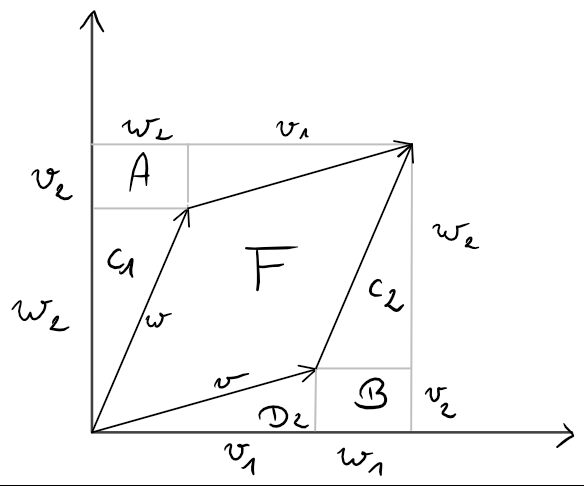
\includegraphics{Parallelogram1.png}\\
Sei F der Flächeninhalt des Parallelogramms und die weiteren Großbuchstaben bezeichnen die Fläche der Recht- bzw. Dreieckflächen. Dann:
\[F=(v_1+w_1)*(v_2+w_2) - (A+B+C_1+C_2+D_1+D_2)\]\[=v_1v_2+w_1v_2+v_2w_2+w_1w_2-(2v_2*w_1+w_1w_2+v_1v_2)\]\[=v_1w_2-v_2w_1 = det\left(
\begin{array}{cc}
v_1&w_1\\
v_2&w_2\\
\end{array}
\right)\] 
\section{Beispiel}
Wir betrachten das Lin-Gleichungssystem $Ax=b, A=(a_{ij})_{i,j=1,2}\in K^{2 \times 2} b \in K^2$. $A$ sei invertierbar. Zeilenumformungen (1. Zeile $\rightsquigarrow$ $a_{22}*$1. Zeile - $a_{12}*$2. Zeile; 2.Zeile $\rightsquigarrow$ $a_{11}*$2. Zeile - $a_{21}*$1. Zeile) zeigen: die eindeutige Lösung $x=\left(
\begin{array}{c}
x_1\\x_2
\end{array}
\right)$ löst auch:\[(a_{11}a_{22}-a_{12}a_{21})x_1=a_{22}b_1-a_{12}b_2\]
\[(a_{11}a_{22}-a_{12}a_{21})x_2=a_{11}b_2-a_{21}b_1\]
Man überprüft leicht, dass $A$ invertierbar ist, genau dann, wenn $det(A) \neq 0$ (s. Folgerung 9.9).\\
Also:\[x_1=\frac{1}{det(A)}det\left(\begin{array}{cc}
b_1&a_{12}\\
b_2&a_{22}
\end{array}
\right),
x_2=\frac{1}{det(A)}det\left(\begin{array}{cc}
a_{11}&b_1\\
a_{21}&b_2
\end{array}
\right)\]
Dies ist der einfachste Fall der \textbf{Cramerschen Regel}.
\section{Definition}
Sei $K$ ein Körper und $n\in \mathbb{N}$. Eine Abbildung \[det: K^{n \times n} \to K\] wird \textbf{Determinante} genannt, falls
\begin{description}
\item[(D1)] $det$ ist linear in jeder Zeile, d.h. für jedes $i=1,...,n$ gilt:
\[det\left(
\begin{array}{c}
a_1\\\vdots\\a_{i-1}\\a_i+b_i\\a_{i+1}\\\vdots\\a_n
\end{array}
\right) = det\left(
\begin{array}{c}
a_1\\\vdots\\a_{i-1}\\a_i\\a_{i+1}\\\vdots\\a_n
\end{array}
\right)+ det \left(
\begin{array}{c}
a_1\\\vdots\\a_{i-1}\\b_i\\a_{i+1}\\\vdots\\a_n
\end{array}
\right)\]
\[det\left(
\begin{array}{c}
a_1\\\vdots\\a_{i-1}\\\lambda a_i\\a_{i+1}\\\vdots\\a_n
\end{array}
\right) = \lambda det\left(
\begin{array}{c}
a_1\\\vdots\\a_{i-1}\\a_i\\a_{i+1}\\\vdots\\a_n
\end{array}
\right)\]
Hierbei sind $a_1,...,a_n,b_i \in K^{1\times n}$ Zeilenvektoren und $\lambda \in K$.
\item[(D2)] $det$ ist alternierend, d.h. hat A zwei gleiche Zeilen, so ist $det(A) = 0$
\item[(D3)] $det$ ist normiert, d.h. $det(E_n) = 1$
\end{description}
\section{Bemerkung}
Für $n=2$ prüft man leicht nach, dass \[\left(
\begin{array}{cc}
a&b\\c&d
\end{array}
\right) \mapsto a*d-b*c\] eine Determinante definiert.\\
Für $n=3$ definiert die \textbf{Sarrus-Regel}
\[det\left(
\begin{array}{ccc}
a_{11}&a_{12}&a_{13}\\
a_{21}&a_{22}&a_{23}\\
a_{31}&a_{32}&a_{33}
\end{array}
\right)\]\[:= a_{11}a_{22}a_{33}+a_{12}a_{23}a_{31}+a_{13}a_{21}a_{32}-a_{31}a_{22}a_{13}-a_{32}a_{23}a_{11}-a_{33}a_{21}a_{12}\]
Man kann zeigen:
\section{Satz}
Zu jedem Körper $K$ und jedem $n\in \mathbb{N}$ existiert eine eindeutig bestimmte Determinante.
\section{Bemerkung}
\begin{description}
\item[i)] Seien $I^n=\left\{\left.
\left(
\begin{array}{c}
x_1\\\vdots\\x_n
\end{array}
\right)\in \mathbb{R}^n \right|0\leq x_i \leq 1
\right\}$ der Einheitswürfel im $\mathbb{R}^n$ und $A\in \mathbb{R}^{n \times n}$ eine Menge der Form $P=\left\{ Ax\left|x\in I^n \right.\right\}$ wird \textbf{Parallelotop} mit Abbildungsmatrix $A$ genannt. Im Fall $n=2$ sind dies gerade Parallelogramme. In Verallgemeinerung zu Beispiel 9.1 gilt für einen geeigneten Volumenbegriff (s. MFI 3): $|det(A)|$ ist das Volumen von $P$.
\item[ii)] Die Verallgemeinerung der Cramerschen Regel für $n>2$ lautet:\\
Ist $A=(a_{ij})_{i,j} \in GL(n,K)$ und $b\in K^n$, so ist die eindeutige Lösung $x\in K^n$ zu $Ax=b$ gegeben durch
\[x_i = \frac{det(a_{\cdot 1},...,a_{\cdot(i-1)},b,a_{\cdot(i+1)},...,a_{\cdot n})}{det(A)}\]
wobei $a_{\cdot j}$ die j-te Spalte von A ist.
\end{description}
\subsection*{Beispiel:}
Das Gleichungssystem:
\[\left(
\begin{array}{ccc}
1&1&0\\
0&1&1\\
3&2&1
\end{array}
\right)*x = 
\left(
\begin{array}{c}
1\\1\\0
\end{array}
\right)\] soll gelöst werden. Mit der Sarrus-Regel berechnet man:
\[det\left(\begin{array}{ccc}
1&1&0\\
0&1&1\\
3&2&1
\end{array}
\right)=2,det\left(\begin{array}{ccc}
1&1&0\\
1&1&1\\
0&2&1
\end{array}
\right)=-2\]
\[det\left(\begin{array}{ccc}
1&1&0\\
0&1&1\\
3&0&1
\end{array}
\right)=4,det\left(\begin{array}{ccc}
1&1&0\\
0&1&1\\
0&2&0
\end{array}
\right)=-2\]
Also:
\[x=\left(\begin{array}{c}
-1\\2\\-2
\end{array}\right)\]
\section{Satz}
Für $det:K^{n\times n} \to K$ gilt:
\begin{description}
\item[i)] Entsteht $B$ aus $A$ durch eine Zeilenvertauschung, so gilt: $det(B) = -det(A)$
\item[ii)] Entsteht $B$ aus $A$ durch Addition des $\lambda$-fachen der j-ten Zeile zur i-ten Zeile ($i \neq j, \lambda \in K$), so: $det(B)=det(A)$
\item[iii)] Ist A eine obere Dreiecksmatrix, also:
\[A=\left(
\begin{array}{cccc}
\lambda_1&*&\cdots&*\\
&\ddots&&\vdots\\
&&\ddots&*\\
0&&&\lambda_n
\end{array}
\right)\]
Dann gilt: $det(A)=\lambda_1 ... \lambda_n$
\end{description}
\subsection*{Beweis}
\begin{description}
\item[i)] Es werde die i-te mit der j-ten Zeile vertauscht ($i \neq j$). Zur Vereinfachung der Notation schreiben wir nur die relevanten Zeilen:
\[det(A) + det(B) = det\left(\begin{array}{c}
a_i\\a_j
\end{array}
\right)+ det\left(\begin{array}{c}
a_j\\a_i
\end{array}
\right)\]
\[\underbrace{=} _{D2}det\left(\begin{array}{c}
a_i\\a_j
\end{array}
\right)+det\left(\begin{array}{c}
a_i\\a_i
\end{array}
\right)+ det\left(\begin{array}{c}
a_j\\a_i
\end{array}
\right)+ det\left(\begin{array}{c}
a_j\\a_j
\end{array}
\right)\]
\[\underbrace{=}_{D1}det\left(\begin{array}{c}
a_i\\a_j+a_i
\end{array}
\right)+ det\left(\begin{array}{c}
a_j\\a_i+a_j
\end{array}
\right) \]
\[\underbrace{=}_{D1} det\left(\begin{array}{c}
a_i+a_j\\a_i+a_j
\end{array}
\right)\]
\[\underbrace{=}_{D2} 0\]
\item[ii)]
\[det(B) = det \left( \begin{array}{c}
a_i+\lambda a_j\\aj
\end{array}
\right)\]
\[\underbrace{=}_{D1} det(A) + \lambda det\left(
\begin{array}{c}
a_j\\a_j
\end{array}
\right)\]
\[\underbrace{=}_{D2} det(A)\]
\item[iii)] Sind alle $\lambda_i \neq 0$, so folgt durch wiederholtes Anwenden von \textbf{ii)}:
\[det(A) = det\left(
\begin{array}{ccc}
\lambda_1 & &0\\
&\ddots&\\
0&&\lambda_n
\end{array}
\right) \underbrace{=}_{D1} \lambda_1 ... \lambda_n det(E_n) \underbrace{=}_{D3} \lambda_1... \lambda_n\]
\end{description}
Andernfalls wählen wir $i$ maximal mit $\lambda_i = 0$ (d.h. $\lambda_{i+1},...,\lambda_n \neq 0)$. Wiederholtes Anwenden von \textbf{ii)} führt zu:
\[det(A) = det \left(
\begin{array}{ccccccc}
\lambda_1&&&&&&*\\
&\ddots\\
0&&\lambda_{i-1}\\
0&\cdots&\cdots&0&\cdots&\cdots&0\\
&&&&\lambda_{i+1}&&*\\
&&&&&\ddots\\
0&&&&&&\lambda_n
\end{array}
\right) = \underbrace{=}_{D1} = 0\]
\[=\lambda_1...\lambda_n. _\square\]
Satz 9.7 rechtfertigt folgenden Algorithmus zur Berechnung der Determinanten:
\section{Algorithmus}
\begin{description}
\item[Input:] $A\in K^{n\times n}$
\item[Output:] $det(A)$
\item[1.)] Bringe $A$ mit Algorithmus 1.6 auf Zeilenstufenform $\tilde{A} = (\tilde{a}_{ij})_{i,j=1,...,n}$ und merke dabei die Anzahl $k$ der Zeilenumformungen.
\item[2.)] Gebe $(-1)^k \tilde{a}_{11}*...* \tilde{a}_{nn}$ als Output aus.\\
Insbesondere folgt die Eindeutigkeit der Determinante in Satz 9.5.
\end{description}
Der Algorithmus zur Berechnung der Inversen aus Kapitel 4 zeigt:
\[A \ \text{invertierbar} \Leftrightarrow \forall _{i=1,...,n}: \tilde{a}_{ii} \neq 0.\]
Also:
\section{Folgerung}
$A\in K^{n \times n}$ ist invertierbar, genau dann, wenn $det(A) \neq 0$.
\section{Beispiel}
Mit Algorithmus 9.8 berechnen wir:
\[det\left(
\begin{array}{ccc}
0&1&2\\
1&1&0\\
3&2&1\\
\end{array}
\right) = -det\left(
\begin{array}{ccc}
1&1&0\\
0&1&2\\
3&2&1\\
\end{array}
\right) =-det\left(
\begin{array}{ccc}
1&1&0\\
0&1&2\\
0&-1&1\\
\end{array}
\right) \]
\[=-det\left(
\begin{array}{ccc}
1&1&0\\
0&1&2\\
0&0&3\\
\end{array}
\right) = -3 \]
Zum Existenzbeweis der Determinante kann man eine explizite Berechnungsformel, die sogenannte Leibniz-Formel angeben. Dazu sei:\[S_n = \left\{ \sigma : \{1,...,n\} \to \{1,...,n\} \left| \sigma \text{ bijektiv}\right.\right\}\]
die sogenannte \textbf{symmetrische Gruppe} vom Grad n. Ihre Elemente heißen \textbf{Permutationen}. Es sei:
\[sign(\sigma):= \left\{
\begin{array}{ll}
1& \text{, falls } \{(i,j) \in \{1,...,n\}^2| i<j \text{ und } \sigma(i) > \sigma (j)\}\\&\text{ eine gerade Anzahl von Elementen hat}\\
-1&\text{, sonst}
\end{array}
\right.\]
das Vorzeichen von $\sigma$.
\section{Satz (Leibniz Formel)}
Ist $K$ ein Körper und $n \geq 1$, so definiert:\[det:K^{n\times n}\to K: (a_{ij})_{i,j=1,...,n} \mapsto \sum_{\sigma \in S_n} sign(\sigma) a_{1\sigma(1)}...a_{n\sigma(n)}\]
eine und (also die) Determinante.
\subsection*{Beweis:}
Fischer, Lineare Algebra.
\section{Satz (Laplacescher Entwicklungssatz)}
Sei $n\geq 2$ und $A = (a_{ij})_{i,j=1,...,n}\in K^{n \times n}$. Es sei für $i,j \in \{1,...,n\}$ $A'_{ij}$ die $(n-1)\times (n-1)$-Matrix, die entsteht, wenn man aus $A$ die i-te Zeile und j-te Spalte entfernt. Dann gilt: Für beliebiges $i=1,...,n$\[det(A) = \sum^n_{j=1}(-1)^{i+j}a_{ij} det(A'_{ij})\](Entwicklung nach der i-ten Zeile) und für beliebiges $j=1,...,n$
\[det(A) = \sum^n_{i=1}(-1)^{i+j} a_{ij} det(A'_{ij})\](Entwicklung nach der j-ten Spalte).
\section{Beispiel}
\[det\left(
\begin{array}{ccc}
0&1&2\\
1&1&0\\
3&2&1
\end{array}
\right)= 0* det\left(
\begin{array}{cc}
1&0\\2&1
\end{array}
\right)+(-1)*1*det\left(
\begin{array}{cc}
1&0\\3&1
\end{array}
\right)+2*det\left(
\begin{array}{cc}
1&1\\
3&2
\end{array}
\right)\]
\[=0-1-2=-3\]
\section{Satz}
Seien $A,B \in K^{n \times n}$. Dann:
\begin{description}
\item[i)] $det(A^T)=det(A)$
\item[ii)] $det(A*B) = det(A)*det(B)$\\
Insbesondere $det(A^{-1}) = (det(A))^{-1}$ für $A\in GL(n,k)$
\end{description}
\subsection*{Beweisskizze}
\begin{description}
\item[ii)] Ist Rang($A$)$<n$, so ist auch $\text{Rang}(A*B)<n$. Nach Folgerung 9.9 sind dann beide Seiten der Gleichung gleich 0. Ist $\text{Rang}(A) = n$ und ist also invertierbar, so gibt es $\tilde{a}_{11},...,\tilde{a}_{nn} \in K\backslash \{0\}$, so dass $A$ aus:\[\left(
\begin{array}{ccc}
\tilde{a}_{11}&&0\\
&\ddots&\\
0&&\tilde{a}_{nn}
\end{array}
\right)\]
durch k-Zeilenvertauschungen und mehrere Additionen von Vielfachen einer Zeile zu einer anderen hervorgeht (man kehre die Umformungen zur Matrixinvertierung von A einfach um). Die Matrix $A*B$ erhält man zuerst für alle $i=1,...,n$, die i-te Zeile von $B$ mit $\tilde{a}_{ii}$ multipliziert und dann die obigen Zeilenumformungen auf die resultierende Matrix anwendet. Also folgt aus Satz 9.7:
\[det(A*B) = (-1)^k det\left(
\begin{array}{c}
\tilde{a}_{11}*b_1\\
\vdots\\
\tilde{a}_{nn}*b_n
\end{array}
\right) \underbrace{=}_{D1} (-1)^k \tilde{a}_{11}...\tilde{a}_{nn}*det(B)\]
\[=det(A)det(B)\]
\item[i)] Hierzu überlegt man sich, dass bei der Berechnung von $det(A^T)$ mittels der Leibnizformel der Summand zur Permutation $\sigma$ gerade dem Summanden zur Permutation $\sigma^{-1}$ bei der Berechnung von $det(A)$ entspricht.$_\square$
\end{description}
\subsection*{Fragestellung:} Wie kann man die Eigenwerte einer Matrix $A\in K^{n\times n}$ berechnen?\\
Dazu:
\[\lambda \text{ ist Eigenwert zu }A \Leftrightarrow (A-\lambda E_n) \text{ ist nicht invertierbar}\]
\[\underbrace{\Leftrightarrow}_{\text{Folgerung 9.9}} det(A-E_n)=0\]
Wir betrachten die Funktion
\[P_A:K\to K, t\mapsto det(A-tE_n),\]
deren Nullstellen gerade die Eigenwerte von $A$ sind. $P_A$ heißt \textbf{charakteristische Funktion} von $A$. Ist $K = \mathbb{R}$ oder $K=\mathbb{C}$, so ist $P_A$ ein Polynom vom Grad n, das sogenannte \textbf{charakteristische Polynom}. Dies sieht man mittels der Leibniz-Formel(vgl. Übung).
\section{Beispiel}
Ist
\[A=\left(
\begin{array}{ccc}
0&-1&1\\
-3&-2&3\\
-2&-2&3
\end{array}
\right),\]
so folgt mit dem Laplaceschen Entwicklungssatz:
\[P_A(t)=det\left(
\begin{array}{ccc}
-t&-1&1\\
-3&-2-t&3\\
-2&-2&3-t
\end{array}
\right) \]\[= -t\text{ } det\left(
\begin{array}{cc}
-2-t&3\\
-2&3-t
\end{array}
\right)+3\text{ }det\left(
\begin{array}{cc}
-1&1\\
-2&3-t
\end{array}
\right)-2\text{ }det\left(
\begin{array}{cc}
-1&1\\
-2-t&3
\end{array}
\right)\]
\[=-t(-2-t)(3-t)-6t-3(3-t)+6+6+2(-2-t)\]
\[=-t^3+t^2+t-1=-(t-1)^2(t+1)\]
Also sind $\lambda_1=1$ und $\lambda_2=-1$ die Eigenwerte von $A$. Mittels des Gauß-Algorithmus berechnet man die Eigenräume:
\[\text{Eig}(A,1) = \text{Lös}\left(
\left(\begin{array}{ccc}
-1&-1&1\\
-3&-3&3\\
-2&-2&2\\
\end{array}
\right),
\left(
\begin{array}{c}
0\\0\\0
\end{array}
\right)
\right)\]
\[
=\left\{x\in \mathbb{R}^3|-x_1-x_2+x_3=0\right\}
\]
\[
=span\left(
\left(
\begin{array}{c}
1\\0\\1
\end{array}
\right),\left(
\begin{array}{c}
0\\1\\1
\end{array}
\right)
\right)\]
\[\text{Eig}(A,-1) = \text{Lös}\left(
\left(\begin{array}{ccc}
1&-1&1\\
-3&-1&3\\
-2&-2&4\\
\end{array}
\right),
\left(
\begin{array}{c}
0\\0\\0
\end{array}
\right)
\right)\]
\[=span
\left(
\left(
\begin{array}{c}
1\\3\\2
\end{array}
\right)
\right)
\]
Somit ist
\[\mathscr{B}=\left(
\left(
\begin{array}{c}
1\\0\\1
\end{array}
\right),\left(
\begin{array}{c}
0\\1\\1
\end{array}
\right),\left(
\begin{array}{c}
1\\3\\2
\end{array}
\right)\right)\]
eine Basis aus Eigenvektoren. Es folgt, dass $A$ diagonalisierbar ist, präziser ähnlich zu
\[
\left(
\begin{array}{ccc}
1&0&0\\
0&1&0\\
0&0&-1
\end{array}
\right)
\]
\chapter{Prä-Hilberträume und Orthogonalprojektionen}
\section*{Motivation:}
wir wollen Begriffe wie die Länge eines Vektors und den Winkel zwischen Vektoren einführen.
\section{Beispiel}
Für Vektoren $x =\left(
\begin{array}{c}
x_1\\x_2
\end{array}
\right)$ und $y =\left(
\begin{array}{c}
y_1\\y_2
\end{array}
\right) \in \mathbb{R}^2$ definieren wir das "`kanonische Skalarprodukt"' durch\[<x,y> := x_1y_1+x_2y_2\]
Es ist dann
\[\sqrt{<x,x>} = \sqrt{x_1^2+x_2^2}\]
nach Satz von Pythagoras die Länge des Vektors $x$:
\\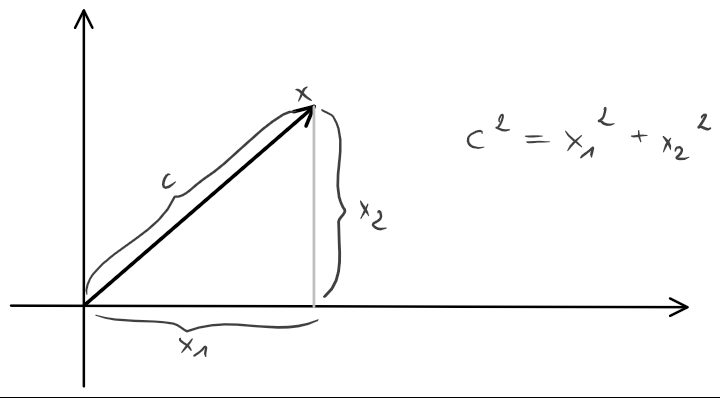
\includegraphics{Graph2.png}
\\
Sei nun $x\neq 0$. Wir setzten
\[\tilde{x} = <x,x>^{-\frac{1}{2}}*x\]
Dann:
\[<\tilde{x},\tilde{x}> = <x,x>^{-1} *(x_1^2+x_2^2) = 1\]
Analog sei für $y\neq 0$
\[\tilde{y} = <y,y>^{-\frac{1}{2}}*y\]
\\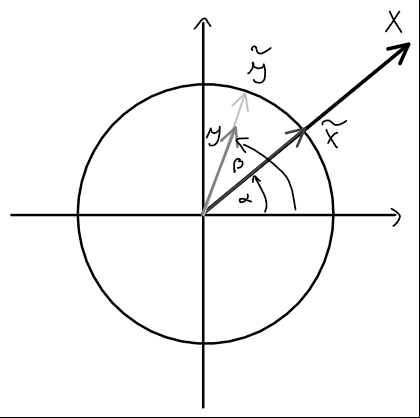
\includegraphics{Graph3.png}
\\
Aus der MfI1 wissen wir: es existieren $\alpha,\beta \in [0,2\pi)$ mit
\[\tilde{x}=\left(
\begin{array}{c}
\cos (\alpha)\\\sin (\alpha)
\end{array}
\right)\]
\[\tilde{y}=\left(
\begin{array}{c}
\cos (\beta)\\\sin (\beta)
\end{array}
\right)\]
Nach dem Additionstheorem für den Kosinus folgt:
\[<x,y> = \sqrt{<x,x>} *\sqrt{<y,y>}(\cos(\alpha)\cos(\beta)+\sin(\alpha)\sin(\beta))\]
\[= \sqrt{<x,x>} *\sqrt{<y,y>} \cos (\beta-\alpha)\]
Wir betrachten das $\varphi \in [0,\pi]$ mit $\cos(\varphi) = \cos(\beta-\alpha)$ als den "`unorientierten Winkel"' zwischen $x$ und $y$. Für ihn gilt:
\[\varphi = \arccos\left(\frac{<x,y>}{\sqrt{<x,x><y,y>}}\right)\]
\section{Definition}
Sei $V$ ein $\mathbb{R}$-VR. Unter einem Skalarprodukt verstehen wir eine Abbildung
\[<\cdot,\cdot>:V\times V \to \mathbb{R}\]
mit
\begin{description}
\item[(S1)] Linearität in der ersten Variablen, d.h.
\[<\lambda v,w> = \lambda<v,w> \text{ und } <v_1+v_2,w >= <v_1,w>+<v_2,w>\]
für alle $v,v_1,v_2,w \in V$ und $\lambda \in \mathbb{R}$
\item[(S2)] Symmetrie:\[<v,w>= <w,v> \text{für alle } v,w \in V\]
\item[(S3)] Positivität:\[<v,v> \geq 0 \text{ und } (<v,v> = 0 \Rightarrow v=0)\]
\end{description}
Ein $\mathbb{R}$-VR versehen mit einem Skalarprodukt wird \textbf{Euklidischer Raum} oder \textbf{Prä-Hilbertraum} genannt.
\section{Bemerkung}
Auf Grund der Symmetrie und der Linearität in der ersten Variable ist ein Skalarprodukt über einem $\mathbb{R}$-VR auch linear in der zweiten Variable, also eine "`Bilinearform"'.
\section{Beispiel}
\begin{description}
\item[i)] In $\mathbb{R}^n$ definiert
\[<x,y> := x^T y = \sum^n_{i=1} x_i y_i\]
ein Skalarprodukt, das sog. kanonische Skalarprodukt oder Euklidische Skalarprodukt im $\mathbb{R}^n$. Zusammen mit diesem Skalarprodukt wird der $\mathbb{R}^n$ auch der n-dimensionale Euklidische Raum genannt.
\item[ii)] Auf dem $\mathbb{R}$-VR $\varphi([a,b],\mathbb{R})$, $-\infty <a <b <\infty$, definiert
\[<f,g> = \int^b_a f(x)g(x) dx\]
ein Skalarprodukt.
\end{description}
\section{Satz (Cauchy-Schwarz-Ungleichung)}
Sei $(V,<\cdot,\cdot >)$ ein Prä-Hilbertraum und $\left\| v\right\| := \sqrt{<v,v>}$. Dann:
\[\left|<v,w>\right| \leq \left\| v\right\| \cdot \left\| w\right\| ,\ v,w\in V\]
Gleichheit gilt genau dann, wenn $v$ und $w$ linear abhängig sind.
\subsection*{Beweis}
Sei $w \neq 0$. Dann gilt für alle $\lambda, \mu \in \mathbb{R}$
\begin{description}
\item[(*)] $0 \leq\ <\lambda v +\mu w, \lambda v +\mu w>$\\
$ = \lambda^2<v,v> +\mu^2<w,w> +2\mu\lambda <v,w>$
\end{description}
Setzt man $\mu := <v,w>$ und $\lambda := <w,w>$ und teilt durch $\lambda >0$, so
\[0 \leq \lambda<v,v> + <v,w>^2 -2<v,w>^2\]
\[= \left\|w\right\|^2\left\|v\right\|^2-<v,w>^2\]
Durch Wurzelziehen folgt die Ungleichung. Falls die Gleichheit gilt, muss das "`$\leq$"' in \textbf{(*)} ein "`$=$"' sein, für die obige Wahl von $\lambda$ und $\mu$. Also:
\[\lambda v +\mu w = 0\]
Da $\lambda >0$, sind $v$ und $w$ linear abhängig.\\
Existiert andererseits ein beliebiges $\left(
\begin{array}{c}
\lambda \\ \mu
\end{array}
\right) \in \mathbb{R}^2 \backslash \{0\}$ mit $\lambda v+ \mu w = 0$, so $v = - \frac{\mu}{\lambda}w$. Also \[\left| <v,w> \right| = \left| \frac{-\mu}{\lambda} \right| <w,w> = \left\|v\right\| \left\| w\right\|,\]
da
\[\left\| v \right\| = \sqrt{<\frac{-\mu}{\lambda} w, \frac{-\mu}{\lambda}w>} = \sqrt{\left(\frac{\mu}{ \lambda}\right)^2 <w,w>} = \left|\frac{-\mu}{\lambda}\right| \sqrt{<w,w>}\]
Ist $w=0$, so sind $v$ und $w$ linear abhängig und beide Seiten der Ungleichung sind gleich Null. $_\square$
\section{Bemerkung}
In einem Prä-Hilbertraum V gilt also:
\[\frac{<v,v>}{\left\|v\right\|\left\|w\right\|} \in [-1,1]\]
Somit können wir in Verallgemeinerung zu Bsp 10.1 den Winkel zwischen $v\neq0$ und $w\neq 0$ definieren durch:
\[\arccos\left(\frac{<v,w>}{\left\|v\right\|\left\|w\right\|}\right)\]
Hierbei ist wieder $\left\| v \right\| := \sqrt{<v,v>}$ die "`Länge"' des Vektors v.\\
Allgemein beschreibt das Konzept der Norm die Länge von Vektoren:
\section{Definition}
Sei V ein $\mathbb{R}$-VR. Eine Abbildung
\[\left\| \cdot \right\| : v \to \mathbb{R}\] wird \textbf{Norm} genannt, falls:
\begin{description}
\item[(N1)] $\left\| \lambda v\right\| = \left| \lambda \right| \left\| v\right\|$ für alle $\lambda \in \mathbb{R}, v \in V$ (positiv homogen)
\item[(N2)] Für alle $v,w \in V$ gilt
\[\left\| v+w \right\| \leq \left\| v\right\| + \left\| w\right\|\] (Dreiecksungleichung)
\item[(N3)] $\left\| v \right\| \geq 0$ und $(\left\| v\right\| = 0 \Rightarrow v= 0)$ (Positivität)
\\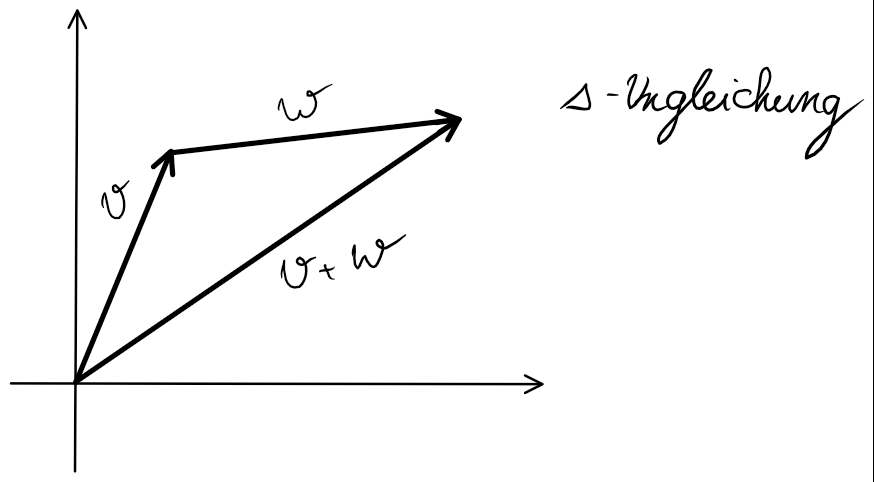
\includegraphics{Graph4.png}
\\
\end{description}
\section{Satz}
Sei $(V.<\cdot,\cdot>)$ ein Prä-Hilbertraum. Dann definiert
\[\| v \| := \sqrt{<v,v>} , v\in V,\]
eine Norm auf V, die von $<\cdot ,\cdot>$ \textbf{induzierte Norm}.
Ferner gilt für alle $v,w \in V$:
\[\| v+w \|^2 = \|v\|^2 + \|w\|^2 + 2<v,w>\text{ \textbf{(P)}}\]
\subsection*{Beweis}
\begin{description}
\item[(N1)] $\|\lambda v\| = \sqrt{<\lambda v, \lambda v>} = \sqrt{\lambda^2 <v,v>} = |\lambda|\|v\|$
\item[(N3)] folgt direkt aus (S3).
\item[(N2)+(P):]
\[\| v+w \|^2 = <v+w,v+w> = <v,v> + <w,w> + 2<v,w>\]
\[\|v\|^2 +\|w\|^2 + 2<v,w>\]
\[\underbrace{\leq}_{\text{Cauchy-Schwarz}} \|v\|^2 + \|w\|^2 + 2\|v\| \|w\|\]
\[=\left(\|v\|+\|w\|\right)^2\ _\square\]
\end{description}
\section{Definition}
Sei $(v,<\cdot,\cdot>)$ ein Prä-Hilbertraum. Dann heißen Vektoren v und w \textbf{orthogonal}, falls $<v,w> = 0$. Nach Bemerkung 10.6 entspricht dies einem Winkel von $\frac{\pi}{2}$ im Bogenmaß, also $90^{\degree}$\\
Eine Familie von Vektoren $(v_1,...,v_n)$ heißt \textbf{orthogonal}, falls für alle $i \neq j$ $v_i$ orthogonal zu $v_j$. Gilt zudem $\|v_i\| = 1$ für alle $i=1,...,n$, so wird die Familie \textbf{orthonormal} genannt. Eine orthonormale Familie, die gleichzeitig Basis von V ist, heißt \textbf{Orthonormalbasis}.
\section{Beispiel}
Die kanonische Basis $\varphi_1,...,\varphi_n$ im $\mathbb{R}^n$ ist eine Orthonormalbasis bzgl. des kanonischen Skalarprodukts.
\section{Satz}
Ist $(v_1,...,v_n)$ orthogonal und $v_i \neq 0$ für alle $i=1,...,n$, so ist $(v_1,...,v_n)$ linear unabhängig.
\subsection*{Beweis}
Sei $\lambda_1 v_1 + \cdots + \lambda_n v_n = 0$ für $\lambda_1,...,\lambda_n \in \mathbb{R}$. Dann:
\[0 = <\sum^n_{i=1} \lambda_i v_i , \sum^n_{k=1} \lambda_k v_k>\]
\[=\sum^n_{i=1} \sum^n_{k=1} \lambda_i \lambda_k \underbrace{<v_i,v_k>}_{=0 \text{ für } i\neq k}\] \[= \sum^n_{i=1} \lambda_i^2 \underbrace{<v_i,v_i>}_{>0}\]
Also $\lambda_i^2 = 0$ und somit $\lambda_i = 0$ für alle $i=1,...,n$.$_\square$
\subsection*{Frage:}
Wie kann man Orthonormalbasen konstruieren?
\section{Definition}
Sei $(V,<\cdot ,\cdot >)$ ein Prä-Hilbertraum, $W\subset V$ ein UVR und $v\in V$. Ein Vektor $w_0\in W$ wird \textbf{Orthogonalprojektion} von v auf W genannt, falls
\[<v-w_0,w> = 0 \text{ für alle } w\in W.\]
\\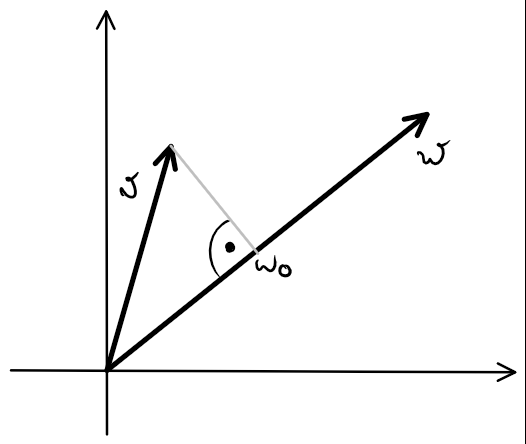
\includegraphics{Graph5.png}
\\
\section{Bemerkung}
Im Existenzfall ist $w_0$ eindeutig bestimmt. Denn ist $\tilde{w}_0$ eine weiter Orthogonalprojektion von v aus W, so gilt für $w = \tilde{w}_0-w_0 \in W$
\[0= <v-w_0,w> - <v-\tilde{w}_0,w> = <\tilde{w}_0-w_o,\tilde{w}_0-w_0>\]
Also: $\tilde{w_0} - w_0 = 0$ nach (S3).\\
Wir beschreiben im Folgenden: $\Pi_W(v) = w_0$.
offensichtlich gilt: $\Pi_W(w) = w$ für alle $w \in W$.
\section{Satz}
Sei $(V,<\cdot ,\cdot >)$ ein Prä-Hilbertraum und $W\subset V$ ein n-dimensionaler Unterraum $(n\in \mathbb{N})$. Dann:
\begin{description}
\item[i)] W hat eine Orthonormalbasis $(w_1,...,w_n)$
\item[ii)] für jedes $v \in V$ und jede Orthonormalbasis $(w_1,...,w_n)$ von W gilt:
\[\Pi_W(v) = \sum^n_{i=1}<v,w_i>w_i\]
Insbesondere ist: $\Pi _W :V \to W$ linear.
\end{description}
\subsection*{Beweis}
\begin{description}
\item[ii)] Sei $(w_1,...,w_n)$ eine Orthonormalbasis von W. Sei zunächst $w \in W$. Dann:
\[w= \sum^n_{i=1} \lambda_i w_i\]
für gewisse $\lambda \in \mathbb{R}$. Es gilt für alle $k = 1,...,n$
\[<w,w_k> = \sum^n_{i=1}\lambda_i \underbrace{<w_i,w_k>}_{=\left\{
\begin{array}{cl}
0,& i\neq k\\
1,& i=k 
\end{array}
\right.} = \lambda_k\]
Sei nun $v\in V$. Dann folgt für alle $w \in W$
\[
<v-\sum^n_{i=1}<v,w_i>w_i,w>
\]
\[
=<v-\sum^n_{i=1}<v,w_i> w_i,\ sum^n_{k=1} <w,w_k>w_k>
\]
\[
=\sum^n_{k=1}<w,w_k><v,w_k>-\sum^n_{i=1}\sum^n_{k=1}<v,w_i><w,w_k>\underbrace{<w_i,w_k>}_{=\left\{
\begin{array}{cl}
0,& i\neq k\\
1,& i=k 
\end{array}
\right.}\]
\[=0\]
Also: \[\Pi_W(v) = \sum^n_{i=1}<v,w_i>w_i\]
\item[i)] Das folgende konstruktive Verfahren heißt \textbf{Gram-Schmidt-Orthonormalisierung}:\\
Sei $(\tilde{w}_1,...,\tilde{w}_n)$ irgendeine Basis von W. Sei $W_k = \text{span}(\tilde{w}_1,...,\tilde{w}_k),\ k=1,...,n$.\\
Definiere:
\[w_1 := \frac{\tilde{w}_1}{\|\tilde{w}_1\|}\]
\[w_k := \frac{\tilde{w}_k - \Pi_{W_{k-1}} (\tilde{w}_k)}{\|\tilde{w}_k - \Pi_{W_{k-1}}(\tilde{w}_k)\|}\]
Wir zeigen induktiv: Für alle $k=1,...,n$ ist $(w_1,...,w_k)$ eine Orthonormalbasis von $W_k$ (und somit ist nach \textbf{ii)} $w_{k+1}$ definiert).
\begin{description}
\item[k=1:] \[ \text{ klar, da } \|w_1\| = \frac{1}{\|\tilde{w}_1\|}\|\tilde{w}_1\|=1\]
\item[k-1 $\rightsquigarrow$ k:] Nach Induktionsannahme ist $(w_1,...,w_{k-1})$ eine orthonormale Familie und $w_l \in W_{k-1}$ für alle $l=1,...,k-1$. Nach Definition der Orthogonalprojektion folgt für alle $l=1,...,k-1$:
\[<w_k,w_l> = \frac{1}{\|\tilde{w}_k-\Pi_{W_{k-1}}(\tilde{w}_k\|} <\tilde{w}_k - \Pi_{W_{k-1}}(\tilde{w}_k)  ,\underbrace{w_l}_{\in W_{k-1}}> =0 \]
Da offensichtlich $\|w_k\| = 1$ und (wegen $W_{k-1} \subset W_k$) auch $w_k \in W_k$, ist $(w_1,...,w_k)$ eine orthonormale Familie in $W_k$. Nach Satz 10.11 ist diese Familie linear unabhängig, also eine Basis, da $dim(W_k)=k$. $_\square$
\end{description}
\end{description}
\section{Beispiel}
\[W = \text{span}(\tilde{w}_1,\tilde{w}_2,\tilde{w}_3) \subset \mathbb{R}^4\]
mit
\[\tilde{w}_1 = \left(
\begin{array}{c}
2\\0\\0\\0
\end{array}
\right),\tilde{w}_2 = \left(
\begin{array}{c}
1\\0\\3\\0
\end{array}
\right),\tilde{w}_3 = \left(
\begin{array}{c}
1\\4\\-2\\3
\end{array}
\right)\]
Seien $W_1 = \text{span}(\tilde{w}_1),W_2 = \text{span}(\tilde{w}_1, \tilde{w}_2)$. Gram-Schmidt-Orthonormalisierung liefert:
\[w_1 = \frac{\tilde{w}_1}{\|\tilde{w}_1\|} = \left(
\begin{array}{c}
1\\0\\0\\0
\end{array}
\right)\]
\[
\tilde{w}_2 - \Pi_{W_{1}}(\tilde{w}_2) = \tilde{w}_2 -<\tilde{w}_2,w_1>w_1
\]
\[
=\left(
\begin{array}{c}
1\\0\\3\\0
\end{array}
\right)
-
\left<
\left(
\begin{array}{c}
1\\0\\3\\0
\end{array}
\right)
,
\left(
\begin{array}{c}
1\\0\\0\\0
\end{array}
\right)
\right>
*
\left(
\begin{array}{c}
1\\0\\0\\0
\end{array}
\right)
=
\left(
\begin{array}{c}
0\\0\\3\\0
\end{array}
\right)
\]
nach Satz 10.14(ii).\\
Also:
\[w_2 = 
\left(
\begin{array}{c}
0\\0\\1\\0
\end{array}
\right)\]
\[\tilde{w_3} - \Pi_{W_2}(\tilde{w_3} )= \tilde{w_3}-<\tilde{w_3},w_1>w_1-<\tilde{w_3},w_2>w_2\]
\[= \left(
\begin{array}{c}
1\\4\\-2\\3
\end{array}
\right)
-
\underbrace{\left<
\left(
\begin{array}{c}
1\\4\\-2\\3
\end{array}
\right)
,
\left(
\begin{array}{c}
1\\0\\0\\0
\end{array}
\right)
\right>}
_{=1}
\left(
\begin{array}{c}
1\\0\\0\\0
\end{array}
\right)
-
\underbrace{\left<
\left(
\begin{array}{c}
1\\4\\-2\\3
\end{array}
\right)
,
\left(
\begin{array}{c}
0\\0\\1\\0
\end{array}
\right)
\right>}
_{=-2}
\left(
\begin{array}{c}
0\\0\\1\\0
\end{array}
\right)
\]
\[
=\left(
\begin{array}{c}
0\\4\\0\\3
\end{array}
\right),
\]
da $(w_1,w_2)$ eine Orthonormalbasis von $W_2$ ist.\\
Da
\[\left\| \left(
\begin{array}{c}
0\\4\\0\\3
\end{array}
\right)\right\| = \sqrt{0^2+4^2+0^2+3^2} =5\]
folgt:
\[
w_3 = \frac{1}{5} \left(
\begin{array}{c}
0\\4\\0\\3
\end{array}
\right)
\]
Also ist
\[\left(
\left(
\begin{array}{c}
1\\0\\0\\0
\end{array}
\right),\left(
\begin{array}{c}
0\\0\\1\\0
\end{array}
\right),
\frac{1}{5}\left(
\begin{array}{c}
0\\4\\0\\3
\end{array}
\right)
\right)\]
eine Orthonormalbasis von W.\\
Die Orthogonlprojektion hat folgende wichtige Minimierungseigenschaft:
\section{Satz}
Sei $(V,<\cdot , \cdot >)$ ein Prä-Hilbertraum mit induzierter Norm $\| \cdot \|$. Sei $W \subset V$ ein endlich dimensionaler Unterraum. Dann existiert zu jedem $v \in V$ genau ein $w_0 \in W$ mit 
\[
\|v-w_0\| = inf _{w\in W} \|v-w\|
\]
und es gilt: $w_0 = \Pi_{W^{(v)}}$
\\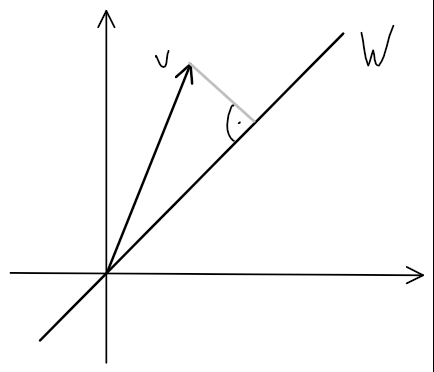
\includegraphics{Graph6.png}
\\
\subsection*{Beweis}
\[\|v-w\|^2 = \|(v-\Pi_{W^{(v)}})+(\Pi_{W^{(v)}}-w)\|^2\]
\[\underbrace{=}_{P} \| v-\Pi_{W^{(v)}} \|^2 + \|\Pi_{W^{(v)}} -w\|^2 + \underbrace{2<v-\Pi_{W^{(v)}}, \underbrace{\Pi_{W^{(v)}} -w}_{\in W}>}_{=0}\]
\[
= \| v -\Pi_{W^{(v)}}\|^2 + \|\Pi_{W^{(v)}} -w\|^2
\]
Dieser Ausdruck wird minimal in w, genau dann, wenn $\| \Pi_{W^{(v)}} -w \| = 0$, was gleichbedeutend mit $w = \Pi_{W^{(v)}}$ ist. $_\square$
\subsection*{Anwendung auf lineare Gleichungssysteme}
Wir betrachten lineare Gleichungssysteme
\[Ax = b , \text{ } A\in \mathbb{R}^{m \times n}, b\in \mathbb{R}^m, m>n.\]
Wir nehmen an, dass $\text{Rang}(A)=n$. Nach Satz 4.11 gilt:
\\Entweder hat $Ax = b$ genau eine Lösung $x = x(b)$ oder es existiert keine Lösung. Im letzteren Fall betrachten wir das Problem.
\\Finde $x_0 \in \mathbb{R}^n$ so, dass 
\[\|Ax_0-b\|\]
minimal wird ($\| \cdot \|$ die vom Euklidischen Skalarprodukt induzierte "`Euklidische Norm"' auf $\mathbb{R}^m$). Es gilt nach Satz 10.16
\[inf_{x \in \mathbb{R}^n} \|Av-b\| = inf_{y \in Im(F_A)} \|y-b\|\]
\[
= \| \Pi_{Im(F_A)}(b)-b\|
\]
Sei $b_0 := \Pi_{Im(F_A)}(b)$. Dann: $b_0 = Ax(b_0)$.\\
Also:
\[
inf_{x \in \mathbb{R}^n} \|Ax-b\| ? \|Ax(b_0)-b\|
\]
Wir finden also die "`beste Approximation"' $x_0$ zu $Ax = b$, indem wir zunächst $b$ orthogonal auf $Im(F_A)$ projizieren und dann die Lösung $x_0$ zu
\[Ax = \Pi_{Im(F_A)} (b)\]
bestimmen.
Wir geben eine explizite Form für $x_0$ an. Da
\[
A^TAx = 0 \Rightarrow x^TA^TAx = 0
\]
\[
\Rightarrow (Ax)^T(Ax) = 0 \Rightarrow \|Ax\| = 0 \Rightarrow Ax = 0
\]
\[
\Rightarrow x = 0,
\]
ist $A^TA$ invertierbar nach Satz 4.13. Sei $y \in Im(F_A)$, also $y = Ax$ für $x \in \mathbb{R}^n$. Dann gilt für alle $b \in \mathbb{R}^m$:
\[<b,y> = <Ax,b> = (Ax)^Tb = x^TA^Tb = x^TA^TA(A^TA)^{-1}A^Tb\]
\[=\underbrace{(Ax)^T}_{=y} A(A^TA)^{-1} A^Tb = <A(A^TA)^{-1}A^Tb,y>.\]
Da $y \in Im(F_A)$ beliebig, folgt \[\Pi_{Im(F_A)}(b) = A(A^TA)^{-1}A^Tb\]
Man nennt $A^+ := (A^TA)^{-1}A^T$ die \textbf{Pseudoinverse} von A. Es ist dann also
\[x_0 = A^+b\] die Bestapproximation zu $Ax=b$.\\
Als Folgerung der obigen Überlegungen halten wir fest:
\section{Satz}
Sei $(\mathbb{R}^m,<\cdot,\cdot>)$ der $m$-dimensionale Euklidsche Raum und W ein $n$-dimensionaler Unterraum des $\mathbb{R}^m$ mit Basis $(w_1,...,w_n)$. Dann gilt für alle $v \in \mathbb{R}^m$:
\[
\Pi_W(v) = \sum^n_{i=1}<A^+v,e_i>w_i,
\]
wobei $A \in \mathbb{R}^{m \times n}$ als Spalten $w_1,...,w_n$ hat und $e_i$ der i-te kanonische Einheitsvektor.
\subsection*{Beweis}
Dann ist $W = Im(F_A)$. Also folgt:
\[
\Pi_W(v) = \Pi_W(Im(F_A))(v) = A A^+ v
\]
\[
=A(\sum^n_{i=1}<A^+v,e_i>e_i) = \sum^n_{i=1}<A^+v,e_i>w_i) _\square
\]
\chapter{Fourierreihen}
\section*{Ziel:}
Approximation einer Funktion durch Überlagerung von Kosinus- und Sinusschwingungen. Dadurch kann ein Signal in die Anteile der einzelnen Frequenzen zerlegt werden.\\
In diesem Kapitel bezeichnet $V = \phi([-\pi , \pi])$ der $\mathbb{R}$-VR der stetigen Funktion $f:[-\pi,\pi] \to \mathbb{R}$ versehen mit dem Skalarprodukt
\[<f,g> := \int^{+\pi}_{-\pi} f(x)g(x) dx\]
Für jedes $n\in \mathbb{N}$ sei
\[W_n := \text{span}(1,\cos(\cdot),\cos(2\cdot) , ..., \cos(n\cdot), \sin (\cdot) , \sin(2\cdot),...,\sin(n \cdot)),\]
wobei etwa $\cos(k\cdot) : [-\pi,\pi] \to \mathbb{R}, x \mapsto \cos(kx)$. Die Elemente von $W_n$ heißen \textbf{trigonometrische Polynome} vom Grad $\leq n$.
\section{Satz}
Für alle $n \in \mathbb{N}$ ist 
\[(1,\cos(1\cdot),...,\cos(n\cdot),sin(\cdot),...,\sin(n\cdot))\]
eine orthogonale Familie in V und also eine Basis von $W_n$.
\subsection*{Beweis}
Da das System $W_n$ erzeugt und die lineare Unabhängigkeit aus der Orthogonalität folgt (Satz 10.11) ist nur die Orthogonalität zu zeigen.\\
Man beachte für alle $l \in \mathbb{Z} \backslash \{0\}$
\[\int^{+\pi}_{-\pi} \cos(lx)dx = [\sin(lx) * \frac{1}{l}]^\pi_{-\pi} = 0\]
\[\int^{+\pi}_{-\pi} \sin(lx)dx = [\cos(lx) * \frac{-1}{l}]^\pi_{-\pi} = 0\]
Ferner folgt aus dem Additionstheoremen für Sinus und Kosinus:
\[\sin((l+m)x) + \sin ((l-m)x)\]
\[= \sin(lx) \cos(mx) + \cos(lx) \sin(mx) + \sin(lx) \cos(mx) \]
\[=-\sin(mx) \cos(lx) = 2\sin(lx) \cos(mx)\]
und analog:
\[ \cos((l+m)x) + \cos((l-m)x) = 2 cos(lx)cos(mx)\]
Also gilt für $l,m >0$:
\[<1,\cos(m \cdot)> = \int^\pi_{-\pi} \cos(mx)dx = 0\]
\[<1,\sin(l \cdot)> = \int^\pi_{-\pi} \sin(lx)dx = 0\]
\[<\sin(l \cdot),\cos(m \cdot)> = 
\frac{1}{2} \int^{\pi}_{-\pi}(\sin((l+m)x)+\sin((l-m)x))dx\]
\[ = 0 \]
(unter beachtung von $\sin(0) = 0$ im Fall $l=m$).
\[<\cos(l\cdot),\cos(m\cdot)> = \frac{1}{2} \int^\pi_{-\pi} (\cos((l+m)x) + \cos((l-m)x) )dx\]
\[= \left\{ 
\begin{array}{cl}
0 & l\neq m\\
\pi & l=m
\end{array}
\right.\]
(unter Beachtung von $\cos(0) = 1$ im Fall $l=m$).
\[<\sin(l\cdot),\sin(m\cdot)> =\int^\pi_{-\pi} \sin(lx) \sin(mx) dx\]
\[=\int^\pi_{-\pi} \cos(lx) \cos(mx) dx - \underbrace{=\int^\pi_{-\pi} \cos((l+m)x) dx}_{=0}\]
\[<\cos(l\cdot), \cos(m\cdot)>\]
\[= \left\{ 
\begin{array}{cl}
0 & l\neq m\\
\pi & l=m
\end{array}
\right.\]
\section{Bemerkung}
Berechnet man noch
\[<1,1> = 2\pi,\]
so folgt, dass
\[(\frac{1}{\sqrt{2\pi}}, \frac{1}{
\sqrt{\pi}} \cos(\cdot),...,\frac{1}{\sqrt{\pi}}\cos(n\cdot),\frac{1}{\sqrt{\pi}}\sin(\cdot),..., \frac{1}{\sqrt{\pi}} \sin(n\cdot))\]
eine Orthonormalbasis von $W_n$ ist.\\
Sei $f\in V$ beliebig. Dann gilt nach Satz 10.14 ii):
\[\Pi_{W_n}(f)\] \[= <f, \frac{1}{\sqrt{2\pi}}>\frac{1}{\sqrt{2\pi}} + \sum^n_{l=1}<f,\cos(l\cdot)\cdot \frac{1}{\sqrt{\pi}}> \frac{1}{\sqrt{\pi}}\cos(l\cdot) + \sum^n_{l=1}<f,\sin(l\cdot)\frac{1}{\sqrt{\pi}}>\frac{1}{\sqrt{\pi}}\sin(l\cdot)\]\[ = \frac{a_0(f)}{2} + \sum^n_{l=0} (a_l(f)\cos(l\cdot)+ b_l(f)\sin(l\cdot))
\]
mit
\[
a_l(f) = \frac{1}{\pi} \int^\pi_{-\pi} f(x) \cos(lx)dx, l = 0, ...,n.\]
\[b_l(f) = \frac{1}{\pi} \int^\pi_{-\pi} f(x) \sin(lx)dx, l = 1, ...,n.
\]
Die Koeffizienten $a_l(f),b_l(f)$ werden \textbf{Fourier-Koeffizienten} von f genannt.\\
Nach Satz 10.16 ist dies die Bestapproximation von $f$ durch trigonometrische Polynome vom Grad $\leq n$ in dem Sinn, dass für alle $g \in W_n$
\[
\int^\pi_{-\pi} \left| 
f(x) - \left(
\frac{a_0(f)}{2} + \sum^n_{l=1} a_l(f) \cos(lx) + b_l (f) \sin(lf)
\right)
\right|^2 dx
\]
\[
\leq \int^\pi_{-\pi} |f(x) -g(x)| ^2 dx
\]
\section{Beispiel}
Sei $f: [-\pi , \pi] \to \mathbb{R}, x \mapsto |x|$. Dann: $f \in V$ und $f$ ist gerade, d.h. $f(x) = f(-x)$.
Also:
\[
\int^0_{-\pi} f(x) \sin(lx)dx = \int^\pi_0 f(-x) \sin(-lx)dx
\]
\[
= - \int^\pi_0 f(x) \sin (lx)dx,
\]
d.h. $b_l(f) = 0$ für alle $l \geq 1$.\\
Ferner gilt für $l \geq 1$:
\[
\frac{1}{\pi} \int^\pi_{-\pi} f(x)\cos(lx) dx = \frac{2}{\pi} \int^\pi_0 f(x) ßcos(lx)dx
\]
\[
\frac{2}{\pi} \int^\pi_0 x \cos(lx) dx
\]
\[
= \frac{2}{\pi} \left(
\left[
x  \frac{\sin(lx)}{l}
\right]^\pi_{0} - \int^\pi_0 \frac{\sin(lx)}{l}dx
\right)
\]
\[
=\frac{2}{\pi} \left[ 
\frac{\cos(lx)}{l^2}
\right]^\pi_0 = \frac{2}{\pi}((-1)^l-1)\frac{1}{l^2}
\]
Also:
\[
a_l(f) = 
\left\{
\begin{array}{cl}
\pi&,l=0\\ 
\frac{-4}{\pi l^2}&,l \text{ ungerade}\\ 
0 & ,l \text{ gerade}
\end{array}
\right.
\]
Die Bestapproximation von $|x|$ durch ein trigonometrisches Polynom vom Grad n lautet also:
\[\frac{\pi}{2} + \sum^n_{l=1} \frac{2}{\pi l^2}((-1)^l-1)\cos(lx)\]
Da $\sum^\infty_{l=1}\frac{4}{\pi}\frac{1}{l^2} < \infty $ , folgt aus dem Majorantenkriterium (MfI1), dass für alle $x \in [-\pi, pi]$ die Reihe
\[
\sum^\infty_{l=1} \frac{2}{\pi l^2} ((-1)^l -1) \cos(lx) = - \sum^\infty_{l=0} \frac{4}{\pi(2l+1)^2} \cos((2l+1)x)
\]
konvergiert. Nach Satz 11.5 und Bemerkung 11.6 (unten) gilt für alls $x \in [-\pi ,\pi]$
\[|x| = 
\frac{\pi}{2} - \sum^{\infty}_{l=0} \frac{4}{\pi(2l+1)^2} \cos((2l+1)x)
\]
Für $x = 0$ erhält man die Identität \[\frac{\pi^2}{8} \sum^\infty_{l=0}\frac{1}{(2l + 1)^2} = 1 + \frac{1}{3^2} + \frac{1}{5^2}+\frac{1}{7^2} + ... \]

\section{Definition (Fourierreihe)} Sei $f\in V$. Unter der \textbf{Fourierreihe} zu f verstehen wir die Folge von \textbf{Fourierpolynomen} 
\[(S_nF)_{n \in \mathbb{N}} \]
mit
\[(S_n f)(x):= \frac{a_0(f)}{2}+\sum^n_{l=0} (a_l(f)\cos(lx) + b_l(f)\sin(lx))\]
und im Konvergenzfall auch den Wert der Reihe
\[(Sf) (x) := \lim_{n \to \infty} (S_nf)(x)\]
\[
= \frac{a_0(f)}{2} + \sum^\infty_{l=1} (a_l(f)\cos(lx)+b_l(f)\sin (lx)).
\]
Mit Techniken aus der Analysis kann man zeigen:
\section{Satz}
Sei $f\in V$. Dann:
\begin{description}
\item[i)] Falls für ein $x \in (-\pi,\pi)$ der Grenzwert $\lim_{n\to \infty}(S_nf)(x)$ existiert, so gilt: $(Sf)(x) = f(x)$, d.h. im Konvergenzfall stellt die Fourierreihe die Funktion dar.
\item[ii)] Falls $f$ an einer Stelle $x \in (-\pi , \pi)$ linksseitig und rechtsseitig dfb. ist, so ex $\lim_{n \to n} (S_nf)(x)$
\item[iii)] $\sqrt{\int^\pi_{-\pi} (f(x)-(S_nf)(x))^2dx} \to 0 (n\to \infty)$, d.h. der Abstand zwischen $f$ und $(S_nf)$ in der von $< \cdot, \cdot>$ induzierten Norm konvergiert gegen 0.
\end{description}
\subsection*{Beweis}
Königsberger, Analysis I, Kapitel 16. $_\square$
\section{Bemerkung}
An den Randpunkten $\pi, -\pi$ gilt: Im Konvergenzfall ist
\[\lim_{n \to \infty}(S_nf)(-\pi) = \lim_{n \to \infty}(S_nf)(\pi)=\frac{f(\pi)f(-\pi)}{2}\]
Und Konvergenz liegt vor, falls $f$ linksseitig dfb. in $\pi$ und rechtsseitig dfb. in $- \pi$ ist.\\Ist $f(\pi) \neq f(-\pi)$, so zeigt $(S_nf)(x)$ in der "`Nähe"' von $-\pi$ und in der "`Nähe"' von $\pi$ ein ausgeprägtes Über-und Unterschwenken, das als Gibbsches Phänomen bekannt ist.
\section{Bemerkung}
Sei $f:[0,\pi] \to \mathbb{R}$ stetig dfb.. Wir ergänzen $f$ zu einer gerade Funktion auf $[-\pi,\pi]$ durch $f(x) := f(-x), x\in [ -\pi,0)$. Sei $x_j := \frac{j-0,5}{n} * \pi, j=1,...,n$. Dann bilden die Punkte $x_j,j=1,...,n$, ein äquidistante Partitionierung des Intervalls $\left[ \frac{0,5 \pi}{n}, \pi-\frac{0,5\pi}{n}\right]$.\\Sei$y = \left(\begin{array}{c}
y_1\\\vdots\\y_n
\end{array}
\right)$ mit $y_i := f(x_j)$. Dann gilt für "`großes"' n:
\[y_j = f(x_j) \approx (S_{n-1}f)(x_j) = \frac{a_0}{2}+ \sum^{n-1}_{k=1} a_k \cos(k \frac{j-0,5}{n}\pi)\]
mit
\[
a_k = \frac{2}{\pi}\int^{\pi}_{0}f(x)\cos(kx)dx \approx \frac{2}{\pi}\sum^n_{l=1}( f(x_l) \cos(kx_l)) \frac{\pi}{n}
\]
\[
= \frac{2}{n} \sum^n_{l=1} y_l \cos(k(l-0,5)\frac{\pi}{n}) =: \text{â}_k(y)
\]
Die Abbildung:
\[\mathbb{R}^n \to \mathbb{R}^n, y \mapsto
\left(
\begin{array}{c}
\text{â}_0(y)\\ \vdots\\\text{â}_{n-1}(y)
\end{array}
\right)
\]
wird \textbf{diskrete Kosinustransformation} genannt. Man überzeugt sich leicht, dass für alle $y \in \mathbb{R}^n$
\[
y_j = \frac{\text{â}_0(y)}{2} + \sum^n_{k=1} \text{â}_k(y) \cos(\frac{\pi}{n} k(j-\frac{1}{2})),j=1,...,n.
\]
vgl. Beispiel 6.3.
\chapter{Orthogonale Matrizen}
\section{Definition}
Eine Matrix $Q \in \mathbb{R}^{n \times n}$ wird \textbf{orthogonal} genannt, falls $Q^TQ = E_n$.\\
Wir bezeichnen die Menge der orthogonalen $n\times n$-Matrizen mit $O(n)$. Sie heißen \textbf{orthogonale Gruppe}
\section{Bemerkung}
\begin{description}
\item[i)]Eine orthogonale Matrix $Q$ ist also gerade eine invertierbare Matrix mit $Q^{-1} = Q^T$
\item[ii)] O(n) ist tatsächlich mit der Matrix-Multiplikation als Verknüpfung eine Gruppe (Übung).
\end{description}
\section{Satz}
Sei $Q \in \mathbb{R}^{n\times n}$ und $<\cdot,\cdot>$ bezeichne das Euklidsche Skalarprodukt auf $\mathbb{R}^n$. Dann sind äquivalent:
\begin{description}
\item[a)] $Q\in O(n)$
\item[b)] Die Spalten von $Q$ sind orthonormal bzgl. $<\cdot,\cdot>$.
\item[c)] Für $x,y \in \mathbb{R}^n$ gilt: $<Qx,Qy> = <x,y>$
\end{description}
Insbesondere erhält Multiplikation mit $Q\in O(n)$ die Länge eines Vektors, d.h. $\| Qx\| = \|x\|$ für alle $x \in \mathbb{R}^n$
\subsection*{Beweis}
\begin{description}
\item[a) $\Leftrightarrow$ b)]: Seien $q_{\cdot i}$ die Spalten von Q. Sei $Q^TQ = (a_{ij})_{i,j=1,...,n}$. Dann: $a_{ij} = <q_{\cdot i},q_{\cdot j}>$, was die Äquivalenz von a) und b) zeigt.
\item[a) $\Leftrightarrow$ c)] Da
\[<Qx,Qy> = (Qx)^TQy = x^T(Q^TQ)y,\]
folgt c) aus a). Andererseits folgt mit $x = e_i, y = e_j$ aus c):
\[a_{ij} = <Qe_i,Qe_j> \underbrace{=}_{c)} <e_i,e_j> = 
\left\{
\begin{array}{cl}
1,&i=j\\
0,&i\neq j
\end{array}
\right.
_\square
 \]
\end{description}
\section{Beispiel}
Sei $n=2$. Dann sind für alle $\alpha \in [0,2\pi)$
\\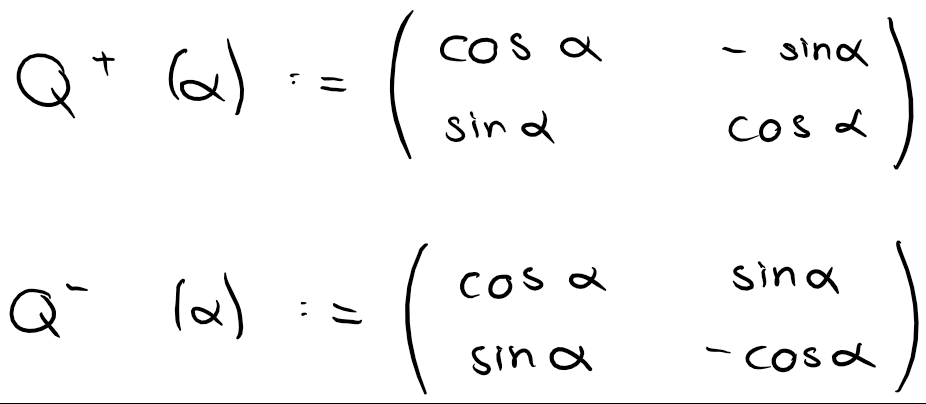
\includegraphics{Beispiel_12_4_1.png}
\\
orthogonal.\\
Die Abbildung $x \mapsto Q^+ (\alpha) *x$ ist eine Drehung um den Winkel $\alpha$, die Abbildung $x \mapsto Q^-(\alpha) *x$ ist eine Spiegelung an der Geraden mit Winkel $\frac{\alpha}{2}$ zur $x_1$-Achse:
\\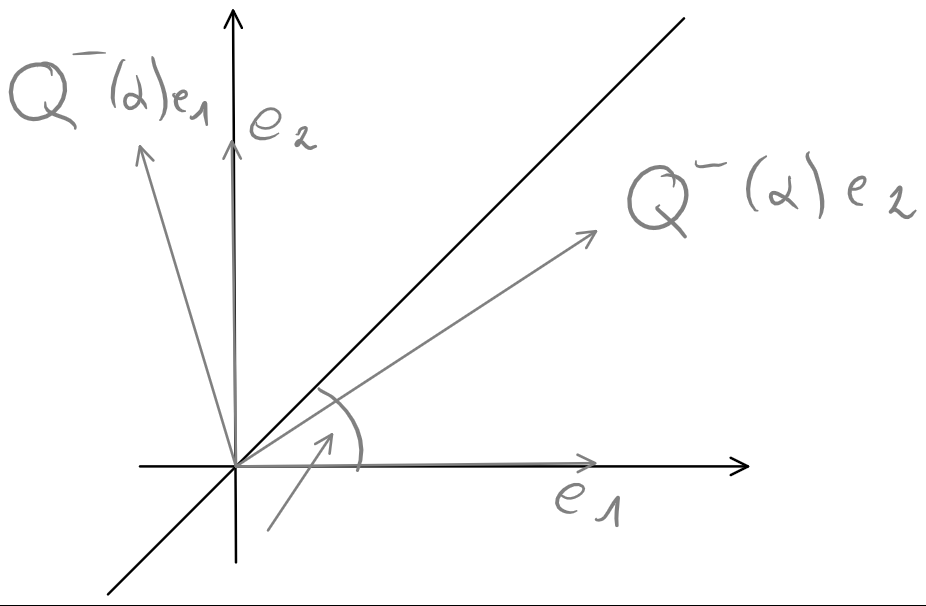
\includegraphics{Beispiel_12_4_2.png}
\\
Wir zeigen, dass dies alle Matrizen in $O(2)$ sind. Sei
\[Q=\left(
\begin{array}{cc}
a&c\\
b&d
\end{array}
\right) \in O(2)\]
Dann: 1.) $a^2+b^2 = 1$, 2.) $c^2+d^2 = 1$, 3.) $a*c+ b*d=0$\\
Wegen 1), 2) existiert $\alpha, \alpha' \in [0,2\pi)$ mit $a = \cos(\alpha)$, $b=\sin(\alpha)$, $c = \cos(\alpha')$, $d = \sin(\alpha')$\\
Aus 3) folgt:
\[\cos(\alpha -\alpha') = \cos(\alpha)\cos(\alpha')+\sin(\alpha)\sin(\alpha')\]
\[=a*c+b*d = 0\]
Also: $\alpha -\alpha' = \frac{\pi}{2} + k \pi$ für ein $k \in \mathbb{Z}$.\\
Somit $c = \cos(\alpha') = \cos(\alpha-(\frac{\pi}{2}+k\pi)) = \sin(\alpha) \sin(\frac{\pi}{2} + k\pi)$\\
$d = \sin(\alpha') = \sin(\alpha-(\frac{\pi}{2}+ kr)) = -\cos(\alpha)sin(\frac{\pi}{2}+kr)$\\
Also:
\[
\left(
\begin{array}{c}
c\\d
\end{array}
\right)
=
\left(
\begin{array}{c}
\sin(\alpha)\\-\cos(\alpha)
\end{array}
\right)
\text{ oder } \left(
\begin{array}{c}
c\\d
\end{array}
\right)
=
\left(
\begin{array}{c}
-\sin(\alpha)\\\cos(\alpha)
\end{array}
\right)\]
da $\sin (\frac{\pi}{2}+ k\pi) \in \{-1,1\}$.
Also: Die Matrizen in $O(2)$ beschreiben genau die Drehungen und Spiegelungen.\\
Sei $Q\in O(n)$. Dann folgt aus den Rechenregeln für die Determinante:
\[det(Q)^2 = det(Q)*det(Q) = det(Q^T)*det(Q)\]
\[det(Q^TQ) = det(E_n) = 1\]
Also: $det(Q) \in \{1,-1\}$.
Man definiert daher:
\[SO(n) := O^+(n) := \{Q\in O(n)|det(Q) = 1\}\]
\[O^- (n) = \{Q\in O(n)|det(Q) = -1\}\]
$SO(n)$ wird \textbf{spezielle orthogonale Gruppe} genannt und ist eine Gruppe bzgl. der Matrixmultiplikation (Übung). Im Fall $n=2$ entsprechen Elemente in $SO(2)$ gerade den Drehungen und sind also "`orientierungserhaltend"'. Elemente in $O^-(2)$ entsprechen den Spiegelungen und sind somit "`orientierungsumkehrend"'.\\
Im allgemeinen Fall $n\in \mathbb{N}$ kann man zeigen (siehe Fischer Abschnitt 5.5.6): \\
\section{Satz(Normalform für orthogonale Matrizen)}
Sei $ Q \in O(n)$. Dann existiert eine $B \in O(n)$ mit\\
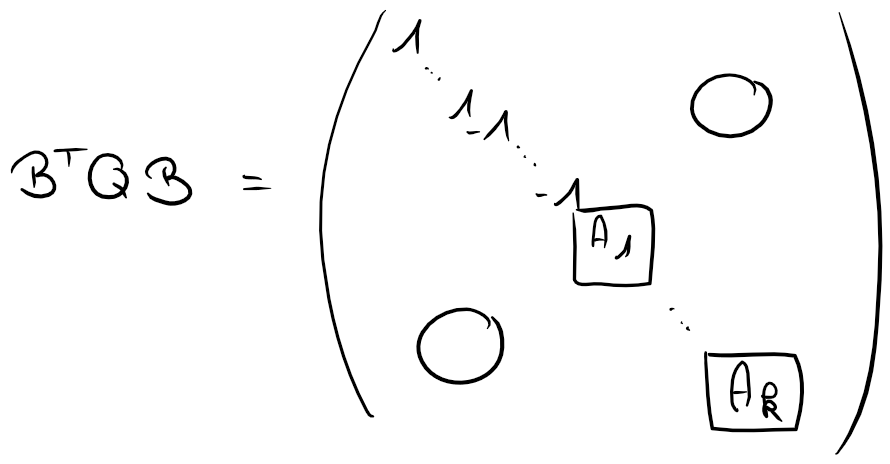
\includegraphics{Satz_12_1_1.png}\\mit\\
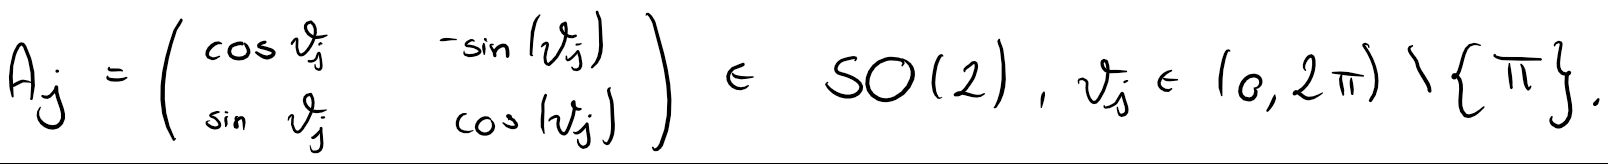
\includegraphics[width=\textwidth]{Satz_12_1_2.png}
\section{Bemerkung}
\begin{description}
\item[i)]Ist $Q \in O(n)$, so sind die einzig möglichen reelen Eigenwerte $1$ und $-1$. Denn aus $Qv = \lambda v (v\neq 0)$, so folgt aus Satz 12.3.
\[\|v\|= \|Qv\| = \|\lambda v\| = |\lambda\| \|v\|\] und also $|\lambda|=1$. Im Satz 12.5. ist die Anzahl von 1-ern auf der Diagonale gleich $dim(Eig(Q,1))$ und die Anzahl der (-1)-er gleich $dim(Eig(Q,-1))$.
\item[ii)]$Q\in SO(n) $ bedeutet, dass in der Normalform der (-1)-Block in der Form
\\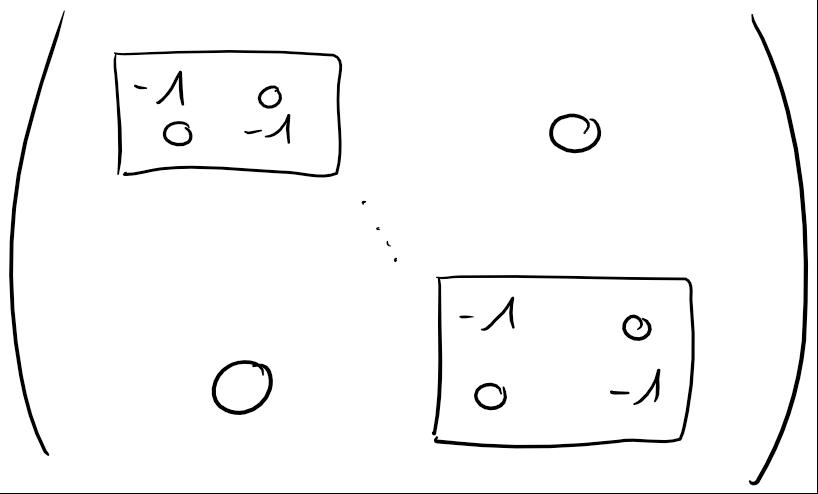
\includegraphics{Bemerkung_12_6_1.png}\\
geschrieben werden kann. Aber $\left(
\begin{array}{cc}
-1&0\\
0&-1
\end{array}
\right)$ entspricht im $\mathbb{R}^2$ einer Drehung um $180 \degree$. Also entspricht Matrix in SO(n) gerade Drehung in 2-dim. Unterräumen, die orthogonal aufeinander stehen.
Entsprechend kann $Q\in O^-(n)$ als Verknüpfung solcher Drehungen mit einer Spieglung interpretiert werden.
\end{description}
\chapter{Symmetrische Matrizen}
\section{Definition (symmetrische Matrix)}
Eine Matrix $A \in \mathbb{R}^{n\times n}$ wird \textbf{symmetrisch} genannt, falls \[A^T = A\]
\section{Lemma}
Ist $A \in \mathbb{R}^{n \times n}$ symmetrisch, so sind alle Eigenwerte von A reell (auch wenn man $A \in \mathbb{C}^{n \times n}$ auffasst.)
\subsection*{Beweis} Sei $Av = \lambda v$ für $\lambda \in \mathbb{C}$ und $v \in \mathbb{C}^n\backslash \{0\}$. Dann: $v = a+ib$ für $a,b \in \mathbb{R}^n $ und wir schreiben $\overline{v} = a-ib$. Dann:
\[
\overline{\lambda} \sum^n_{j=1} (a_j^2 +b_j^2) = \overline{\lambda} v^T \overline{v} = v^T (\overline{\lambda v}) = v^T (\overline{Av})
\]
\[=v^T A \overline{v} = v^TA^T \overline{v} = (Av)^T \overline{v} = (\lambda v)^T \overline{v} = \lambda v^T \overline{v}\]
\[= \lambda(\sum^n_{j=1} a_j^2 + b_j^2)\]
Also: $\lambda = \overline{\lambda}$ (da $v \neq 0$), d.h. $\lambda \in \mathbb{R} _\square$
\section{Satz (Spektraldarstellung für symmetrische Matrizen)}
Sei $A \in \mathbb{R}^{n\times n}$ symmetrisch. Dann ist A über $ \mathbb{R}$ diagonalisierbar.\\Genauer: Es existiert $B \in O(n)$ mit \\
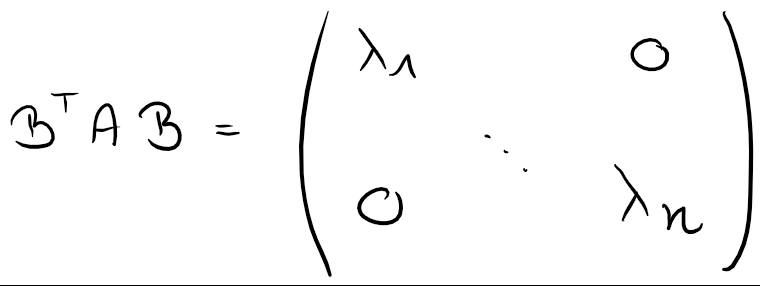
\includegraphics{Satz_13_3_1.png}\\
wobei $\lambda_1,..., \lambda_n \in \mathbb{R}.$\\
Insbesondere bilden die Spalten von $B$ eine Orthonormalbasis aus Eigenvektoren von $A$.
\subsection*{Beweis}
 Wir betrachten A $\in\mathbb{C}^{n \times n}$. Dann zerfällt das charakteristische Polynom von $A$ über $\mathbb{C}$ in Linearfaktoren (nach dem Fundamentalsatz der Algebra):
\[P_A(t) = det(A-tE_n) = \pm (t- \lambda_1) ... (t-\lambda_n)\]
für $\lambda_1,..., \lambda_n \in \mathbb{C}.$\\
Aus Lemma 13.2. folgt, dass $\lambda_1,..., \lambda_n \in \mathbb{R}.$ Insbesondere existiert mindestens ein reeller Eigenwert $\lambda_1$ zu $A$. Der weitere Beweis erfolgt mittels Induktion über n:
\begin{description}
\item[n = 1:] klar
\item[n-1 $\rightarrow$ n:] Nach der Verüberlegung existiert ein Eigenwert $\lambda_1 \in \mathbb{R}$ mit dazugehörigen Eigenvektor $v_1 \in \mathbb{R}^n\backslash \{0\}$, von dem wir annehmen können, dass er auf $\|v_1\|=1$ normiert ist. Hier ist $\|\cdot\|$ die vom Euklidischen Skalarprodukt $<\cdot,\cdot>$ induzierte Norm. Sei
\[W = \{w \in \mathbb{R}^n | <w,v_1> = 0\}.\]
Sei $(\tilde{b_2},...,\tilde{b}_n)$ irgendeine Orthonormalbasis von $W$ (Satz 10.14, Beispiel 5.17). Sei $\tilde{B}$ die $n \times n$-Matrix mit Spalten $v_1, \tilde{b_2},...,\tilde{b_n}$ und $\tilde{B_1}$ die $n \times (n-1)$-Matrix mit Spalten $\tilde{b_2},...,\tilde{b_n}$
Dann ist $\tilde{B} \in O(n)$ und \\
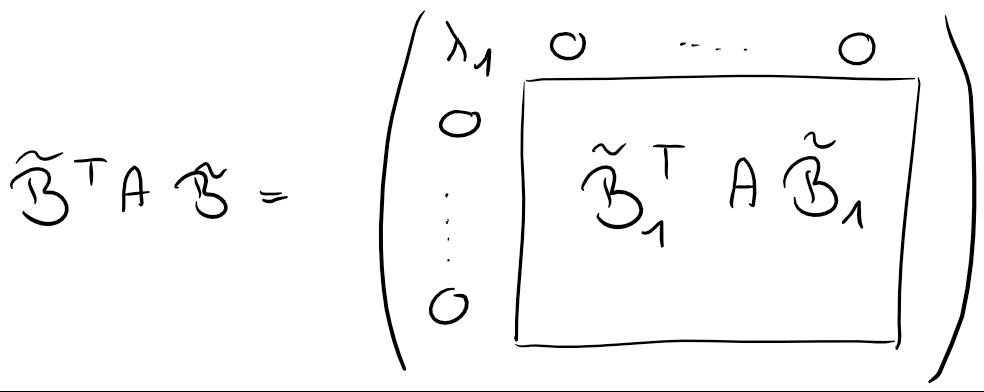
\includegraphics{Beweis_13_3_1.png}\\
Denn: \\
\[
e^T \tilde{B}^TA\tilde{B}e_j = \left\{
\begin{array}{lll}
v_1^TA^T\tilde{b}_j & = \lambda_1 v_1^T \tilde{b}_j = 0& , i=1, j\neq 1\\
\tilde{b}_i^T A v_1 & = \lambda_1 \tilde{b}^T_iv_1 = 0 &, i\neq1, j=1\\
v_1^TAv_1 & = \lambda_1 v_1^Tv_1 = \lambda_1 &,i=j=1\\
\tilde{b}_i^T A \tilde{b}_j& = e_{i-1}^T \tilde{B}_1^T A \tilde{B}_1 e_{j-1} &, i\neq 1, j\neq1\\
\end{array}
\right.
\]
Da $(\tilde{B}_1^T A \tilde{B}_1)^T = \tilde{B}_1^T A^T \tilde{B}_1 = \tilde{B}_1^T A \tilde{B}_1$, ist die Induktionsannahme auf diese Matrix anwendbar und wir erhalten $B_{n-1} \in O(n-1)$ und $\lambda_2,..., \lambda_n \in \mathbb{R}.$ Mit\\
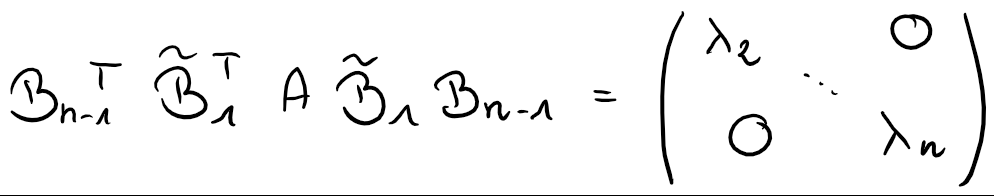
\includegraphics{Beweis_13_3_2.png}\\
Seien $v_2, ..., v_n$ die Spalten von $\tilde{B}_1 B_{n-1}$. Dann gilt für alle $i \neq 1, j \neq 1$:\\
\[<v_1,v_i> = <v_1, \tilde{B}_1 B_{n-1} e_{i-1}> = e_{i-1}^T B_{n-1}^T \underbrace{\tilde{B}_1^T v_1}_{=0} = 0\]
\[<v_j, v_i> = e_{i-1}^T B_{n-1}^T \underbrace{\tilde{B}_1^T \tilde{B}_1}_{= E_{n-1}}B_{n-1}e_{j-1}\]
\[= e_{i-1}^T \underbrace{B_{n-1}^T B_{n-1}}_{=E_{n-1}}e_{j-1}= \left\{
\begin{array}{l}
0, i\neq j\\
1, i=j\\
\end{array}
\right.\]
Also bilden $(v_2, ..., v_n)$ eine Orthonormalbasis von $W$. Sei $B$ die Matrix mit Spalten $v_1,...,v_n$. Also folgt (*) mit $B$ statt $\tilde{B}$, dass $B \in O(n)$ und \\
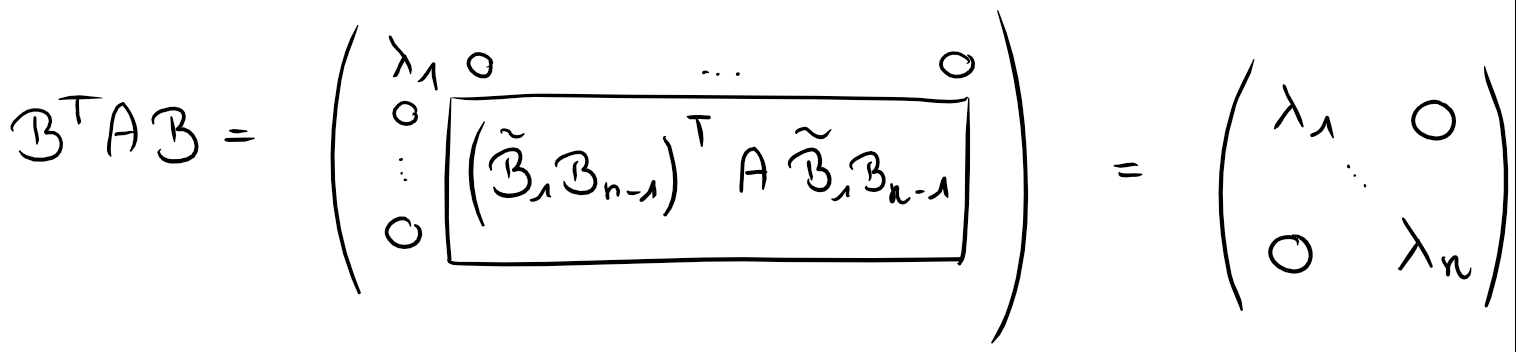
\includegraphics[width=\textwidth]{Beweis_13_3_3.png}\\
$_\square$
\end{description}
\section{Definition}
Eine symmetrische Matrix $A \in \mathbb{R}^{n \times n}$ heißt\begin{itemize}
\item \textbf{positiv(semi-)definit}, falls für alle $x \in \mathbb{R}^n\backslash\{0\} x^TAx > (\geq)0 $
\item \textbf{negativ(semi-)definit}, falls für alle $x \in \mathbb{R}^n\backslash\{0\} x^TAx < (\leq) 0$
\item \textbf{indefinit}, falls A weder positiv semidefinit noch negativ semidefinit ist.
\end{itemize}
\section{Satz}
Für $A \in \mathbb{R}^{n \times n}$ symmetrisch ist äquivalent:
\begin{description}
\item[a)] $A$ ist positiv (semi-) definit
\item[b)] Für alle Eigenwerte $\lambda$ von $A$ gilt: $\lambda > (\geq) 0$
\end{description}
\subsection*{Beweis}
Sei $(v_1,...,v_n)$ eine Orthonormalbasis aus Eigenvektoren zur Matrix $A$ mit zugehörigen Eigenwerten $\lambda_1,...,\lambda_n$ (Satz 13.3). Sei $x \in \mathbb{R}^n\backslash \{0\}$ mit Basisdarstellung $x = \sum^n_{i=1} x_i v_i$. Dann:
\[x^TAx=(\sum^n_{i=1} x_i v_i)^T A (\sum^n_{j=1}x_jv_j)\]
\[=\sum^n_{i=1} x_i v_i^T \sum^n_{j=1}x_j \lambda_j v_j\]
\[ = \sum^n_{i,j=1} x_ix_j\lambda_j \underbrace{v_i^Tv_j}_{
=\left\{
\begin{array}{l}
1, i=j\\
0, i\neq j
\end{array}
\right.
}\]
\[=\sum^n_{i=1} \lambda_i x_i^2\]
\begin{description}
\item[a) $ \Rightarrow$ b)] Ist $ \lambda_j 
\begin{array}{c}
\leq\\
(<)
\end{array} 0$ für ein $j$, so folgt
\[v_j^TAv_j = \lambda_j\begin{array}{c}
\leq\\
(<)
\end{array} 0 \]
Also ist $A$ nicht positiv (semi-)definit.
\item[b) $\Rightarrow$ a)] Ist $\lambda_i \begin{array}{c}
\geq\\
(>)
\end{array} 0$ für alle $i=1,...,n$, so gilt für $x \in \mathbb{R}^n\backslash \{0\}$
\[x^TAx = \sum^n_{i=1} \lambda_i x_i^2 
\begin{array}{c}
\geq\\
(>)
\end{array} 0._\square\]
\end{description}
\section{Beispiel}
Sei $A\in \mathbb{R} ^{m \times n}$ mit Rang $r$. Dann ist $A^TA$ symmetrisch und positiv semidefinit. Denn:
\[x^TA^TAx = (Ax)^TAx = \|Ax\|^2 \geq 0\]
mit der gleichen Argumentation sieht man:
$A^TAx = 0 \Rightarrow \|Ax\|^2 = x^TA^TAx = 0 \Rightarrow Ax = 0$
Also:
\[A^TAx = 0 \Leftrightarrow Ax=0,\]
d.h. Rang $(A^TA) = r$. Nach Satz 13.3 und Satz 13.5 existiert ein $B\in O(n)$ mit 
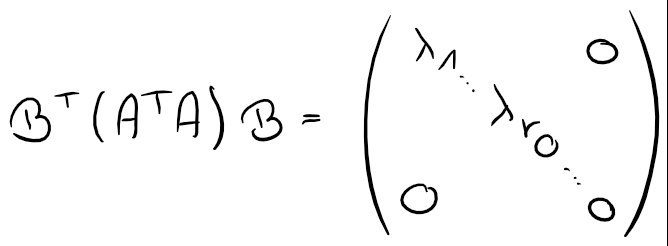
\includegraphics{Beispiel_13_6_1.jpeg}
,wobei
\[\lambda_1 \geq \lambda_2 \geq ... \geq \lambda_r > 0\]
\section{Satz}
Sei $A \in \mathbb{R}^{n \times n}$ symmetrisch und positiv semi definit. Dann existiert eine (eindeutig bestimmte) symmetrische positiv semi definite Matrix $A^{\frac{1}{2}} \in \mathbb{R}^{n\times n}$ mit $A = A^{\frac{1}{2}} A^{\frac{1}{2}}$. $A^{\frac{1}{2}}$ wird \textbf{Quadratwurzel} von $A$ genannt.
\subsection*{Beweis (nur Existez)}
Nach Satz 13.3 existiert $B\in O(n)$ mit\\
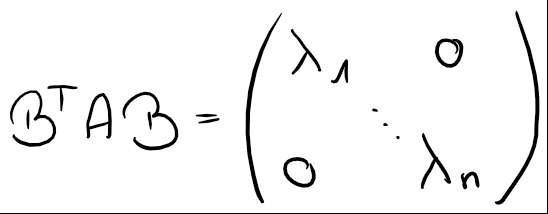
\includegraphics{Beweis_13_7_1.jpeg},\\
wobei $\lambda \geq 0$ nach Satz 13.5 für alle $i=1,...,n$.
Sei\\
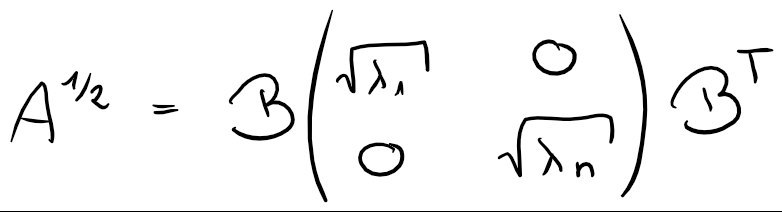
\includegraphics{Beweis_13_7_2.jpeg},\\
Dann:\\
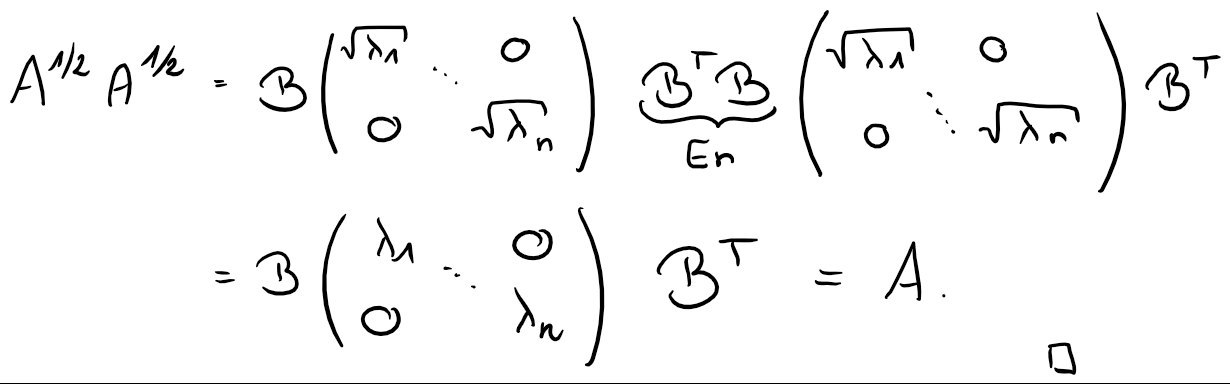
\includegraphics[width=\textwidth]{Beweis_13_7_3.jpeg}.\\
\section{Satz}
Eine symmetrische Matrix $A=(a_{ij})_{i,j} \in \mathbb{R}^{n \times n}$ ist positiv definit genau dann, wenn für alle $k = 1,...,n$
\[det\left(
\begin{array}{ccc}
a_{11}&\cdots&a_{1k}\\
\vdots&\ddots&\vdots\\
a_{k1}&\cdots&a_{kk}\\
\end{array}
\right) >0\]
\section{Beweis}
Die Matrix
\[A = \left(
\begin{array}{ccc}
2&-1&-3\\
-1&2&4\\
-3&4&9
\end{array}
\right)\] ist positiv definit, denn:
\[det(2) = 2 >0\]
\[det\left(
\begin{array}{cc}
2&-1\\
-1&2
\end{array}
\right) = 4-1=3>0\]
\[det\left(
\begin{array}{ccc}
2&-1&-3\\
-1&2&4\\
-3&4&9
\end{array}\right)
=36+12+12-(18+32+9) =1>0
\]
\chapter{Singulärwertzerlegung}
\section{Satz}
Sei $A \in \mathbb{R}^{m \times n}$ vom Rang r. Dann existieren orthogonale Matrizen $U \in O(m) , V \in O(n)$ und $\sigma_1 \geq \sigma_2 \geq ... \geq \sigma_r > 0$ mit\\
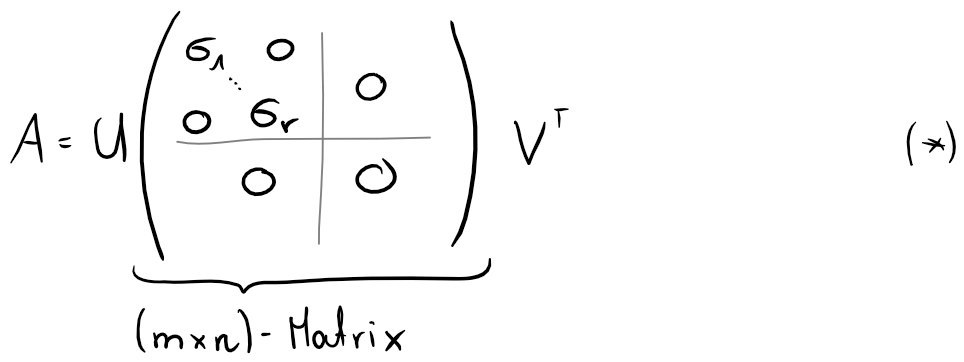
\includegraphics{Satz_14_1_1.jpeg}\\
Die positiven Diagonaleinträge $\sigma_1,...,\sigma_r$ sind eindeutig bestimmt und heißen \textbf{Singulärwerte} von $A$. Eine Darstellung der Form (*) wird \textbf{Singulärwertzerlegung} von $A$ genannt.
\subsection*{Beweis}
Sei $A = U \Sigma V^T$ eine Singulärwertzerlegung von $A$. Dann:
\[A^TA = V\Sigma^T \underbrace{U^TU}_{=E_m} \Sigma V^T = V \Sigma^T \Sigma V^T. \]
Also:
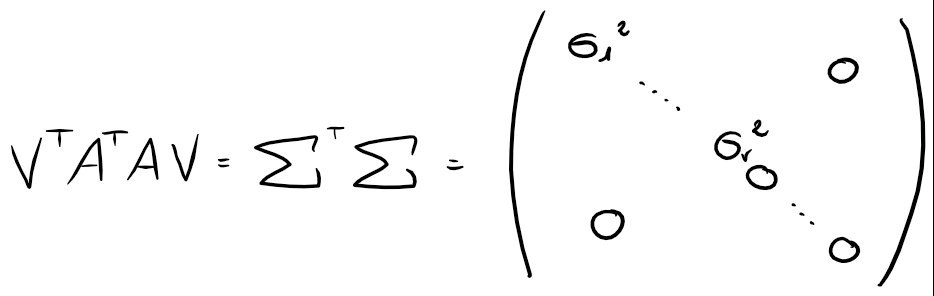
\includegraphics{Beweis_14_1_1.jpeg}\\
Die Singulärwerte sind also die Wurzeln der positiven Eigenwerte von $A^TA$ und also eideutig bestimmt.\\
Zur Konstruktion einer Singulärwertzerlegung:
\begin{description}
\item[Schritt 1:] Diagonalisiere $A^TA$, d.h. finde $V \in O(n)$ und $\lambda_1 \geq \lambda_2 \geq ... \geq \lambda_n \geq 0$ mit\\
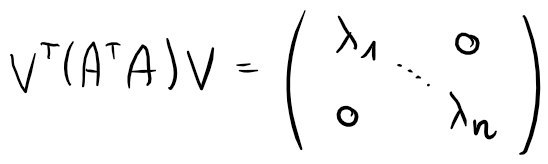
\includegraphics{Beweis_14_1_2.jpeg}\\
\item[Schritt 2:] Für $i=1,...,r$ setze $v_i = V_{e_i}$ (i-te Spalte von $V$) und
\[
u_i = \frac{1}{\sqrt{\lambda_i} }Av_i
\]
und bestimme eine Familie von $(m-r)$ orthonormalen Vektoren $(u_{r+1},...,u_{m})$ im $\mathbb{R}^m$, so dass jeder von diesen orthogonal zu jedem $u_i,i=1,...,r$ ist.
\item[Schritt 3:] Setze $ \Sigma = (s_{ij})_{i=1,...,m,j=1,...,n}$ mit $s_{ii} = \sqrt{\lambda_i}$ für $i=1,...,r$ und $s_{ij} = 0$ sonst. Sei $U$ die Matrix mit Spalten $u_1,...,u_m$. Wir zeigen: $U\Sigma V^T$ ist eine Singulärwertzerlegung von $A$:\\
Für $i,j = 1,...,r$ gilt:
\[u^T_i u_j = \frac{1}{\sqrt{\lambda_i \lambda_j}} e_i^T V^TA^TAVe_j\]
\[\frac{1}{\sqrt{\lambda_i\lambda_j}} e_i^T \lambda_j e_j = \left\{ 
\begin{array}{c}
0, i\neq j\\
1, i=j
\end{array}
\right.\]
Also bilden die Spalten von $U$ ein Orthonormalsystem, d.h. $U \in O(m)$.\\
Ferner:
\[U \Sigma V^T = \sum^r_{i=1} \sqrt{\lambda_i} u_i v_i^T\]
\[=\sum^r_{i=1}Av_iv_i^T = \sum^n_{i=1}Av_iv_i^T\]
\[=A \sum^n_{i=1}v_iv_i^T = AVV^T = AE_n = A. _\square\]
\end{description}
\subsubsection*{Bemerkung}
Im Schritt 2 kann man zuerst $(u_1,...,u_r)$ zu einer Basis $(u_1,...,u_r, \tilde{u}_{r+1},...,\tilde{u}_m)$ des $\mathbb{R}^m$ ergänzen (Basisergänzungssatz) und diese dann mit Gram-Schmidt orthonormalisieren.
\section{Beispiel}
Bestimmt werden soll eine Singulärwertzerlegung von
\[A = \frac{1}{9}\left(
\begin{array}{ccc}
-8&10&14\\
2&2&1\\
-6&-6&-3\\
-16&2&10\\
\end{array}
\right)\]
\begin{description}
\item[Schritt 1:]Man berechnet
\[A^TA = \frac{1}{9}\left(
\begin{array}{ccc}
40&-8 &-28\\
-8&16 &20\\
28&20 &34\\
\end{array}
\right)\]
sowie das charakteristische Polynom
\[det(A^TA -t E_3) = c(t^3-10 t^2 + 16 t),\]
für eine Konstante $c \in \mathbb{R}$. Dieses hat als Nullstellen
\[\lambda1 = 8\]
\[\lambda2 = 2\]
\[\lambda3 = 0\]
Durch Lösen der linearen Gleichungssysteme
\[A^TA - \lambda_j \left(
\begin{array}{ccc}
1&0&0\\
0&1&0\\
0&0&1
\end{array}
\right) = 0\ (j=1,2,3)\]
findet man Eigenvektoren $v_j$ zu $\lambda$ (die man auf Länge 1 normiert), nämlich:
\[
v_1 = \left(\begin{array}{c}
\frac{-2}{3}\\
\frac{1}{3}\\
\frac{2}{3}
\end{array}
\right),
v_2 = \left(\begin{array}{c}
\frac{2}{3}\\
\frac{2}{3}\\
\frac{1}{3}
\end{array}
\right)
v_3 = \left(\begin{array}{c}
\frac{1}{3}\\
\frac{-2}{3}\\
\frac{2}{3}
\end{array}
\right)
\]
\item[Schritt 2]: Man berechnet
\[u_1 = \frac{1}{\sqrt{\lambda_1}} A v_1 = \frac{1}{\sqrt{2}} \left(
\begin{array}{c}
1\\0\\0\\1
\end{array}
\right)\]
\[u_2 = \frac{1}{\sqrt{\lambda_2}} A v_2 = \frac{1}{3\sqrt{2}} \left(
\begin{array}{c}
2\\1\\-3\\-2
\end{array}
\right)\]
Ergänze $(u_1,u_2)$ zu einer Basis des $\mathbb{R}^4$ durch  $(u_1,u_2,e_1,e_2)$.
Das Gram-Schmidt-Verfahren liefert dann:
\[u_3 = \frac{1}{3\sqrt{10}} \left(
\begin{array}{c}
5\\-2\\6\\-5
\end{array}
\right) \]
\[u_4 = \frac{1}{\sqrt{10}} \left(
\begin{array}{c}
0\\3\\1\\0
\end{array}
\right) \]
\item[Schritt 3:] Eine Singulärwertzerlegung von $A$ ist
\[A = \underbrace{\frac{1}{3\sqrt{10}}
\left(
\begin{array}{cccc}
3\sqrt{5} & 2 \sqrt{5}& 5 &0\\
0 &  \sqrt{5} & -2 &9\\
0 &-3\sqrt{5} & 6 & 3\\
3\sqrt{5} & -2\sqrt{5} & -5 & 0
\end{array}
\right)}_{U}\underbrace{\left(
\begin{array}{ccc}
2\sqrt{2}&0&0\\
0&\sqrt{2}&0\\
0&0&0\\
0&0&0
\end{array}
\right)}_{\Sigma}
\underbrace{
\frac{1}{3}
\left(
\begin{array}{ccc}
-2&1&2\\
2&2&1\\
1&-2&2
\end{array}
\right)
}_{V^T}
\]
\end{description}
\section{Bemerkung}
Ist $A \in \mathbb{R}^{m \times n}$ mit $n > m$, so berechnet man zunächst eine Singulärwertzerlegung zu $A^T$: $A^T = \tilde{U} \tilde{\Sigma} \tilde{V}^T$. Dann ist mit $U = \tilde{V}, V = \tilde{U}$ und $\Sigma = \tilde{\Sigma}^T$, so ist $A= \tilde{V} \tilde{\Sigma}^T \tilde{U}^T = U\Sigma V^T$ eine Singulärwertzerlegung von $A$.
\section{Bemerkung}
Ist $A \in \mathbb{R}^{m \times n}$ mit Singulärwertzerlegung
\[
A = U\Sigma V^T
\]
mit\\
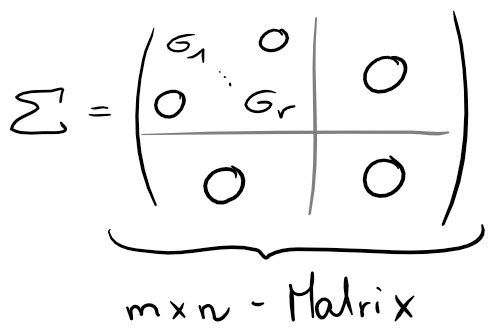
\includegraphics{Bemerkung_14_4_1.jpeg}\\
so schreibt man:
\\
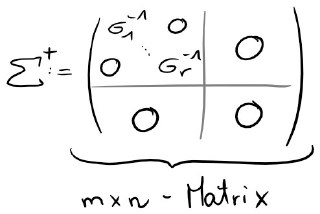
\includegraphics{Bemerkung_14_4_2.jpeg}
\\
\[A^+ = V \Sigma^+ U^T\]
und nennt $A^+$ die \textbf{Pseudo-Inverse} zu A. Ist $m \geq n$ und $Rang(A) = n$, so kann man zeigen, dass\[V \Sigma^+ U^T = (A^TA)^{-1}A^T \] (vgl. Kapitel 10).\\
Es gilt weiterhin für jede rechte Seite $b \in \mathbb{R}^m$
\[\| A(A^+b)-b\| \leq \|Ax-b\| \text{ für alle } x \in \mathbb{R}^n.\]
Ist zudem $\tilde{x} \in \mathbb{R}^n$ mit $ \|A \tilde{x} -b \| = \|A(A^+b)-b\|$, so folgt
\[\|A^+b\| \leq \|\tilde{x} \|.\]
\section{Bemerkung}
Sei $A \in \mathbb{R}^{n\times n}$ invertierbar mit Singulärwerten $\sigma_1 \geq ... \geq \sigma_n > 0$. Dann nennt man
\[\kappa(A) = \frac{\sigma_1}{\sigma_n}\]
die \textbf{Kondition} von $A$ (bzgl. der "`Spektralnorm"'). Man kann zeigen:\\
Sind $b, \tilde{b} \in \mathbb{R}^n$ und $x, \tilde{x} \mathbb{R}^n$ mit $Ax = b$ und $A \tilde{x} = \tilde{b}$, so gilt in der Euklidschen Norm:
\\
\begin{center}

\includegraphics[width = 100px]{Kappa.jpeg}
\end{center}
\[
\| x - \tilde{x} \| \leq \kappa (A) \frac{\|x\|}{\|b\|}\|b-\tilde{b}\|.
\]
Ist die Kondition von A nahe dei 1, so führen kleine relative Fehler in der rechten Seite $\left( \frac{\| b- \tilde{b} \|}{\|b\|} \text{ klein}\right)$ zu kleinen relativen Fehlern bei der Lösung $\left( \frac{\| x- \tilde{x} \|}{\|x\|} \text{ klein}\right)$ so können kleine relative Fehler in der rechten Seite zu großen relativen in der Lösung führen. Bei der Umordnung auf Zeilenstufenform mit dem Gaußalgorithmus kann sich die Kondition drastisch verschlechtern. Im Beispiel 1.10 ist
\[
\kappa \left(
\begin{array}{cc}
10^{-4}&1\\
1&1
\end{array}
\right) \approx 2,62
\]
\[
\kappa \left(
\begin{array}{cc}
10^{-4}&1\\
0&-9999
\end{array}
\right) \approx 10^8
\]
\chapter{Quadriken}
\section{Definiton}
Sei $A \in \mathbb{R}^{n \times n}$ symmetrisch, $b \in \mathbb{R}^n, c \in \mathbb{R}$.
\begin{description}
\item[i)] Eine Abbildung vom $\mathbb{R}^n$ nach $\mathbb{R}$ von der Form
\[x \mapsto x^TAx\] heißt \textbf{quadratische Form}.
\item[ii)] Eine Abbildung vom $\mathbb{R}^n$ nach $\mathbb{R}$ von der Form
\[x \mapsto x^TAx + b^Tx +c\]
heißt \textbf{quadratisches Polynom}.
\item[iii)] Eine Teilmenge des $\mathbb{R}^n$ heißt \textbf{Quadrik}, falls sie Nullstellen eines quatratischen Polynoms ist.
\end{description}
\subsection*{Ziel}
Quatriken sollen auf eine möglichst einfache Form gebracht werden, aus der man ihrer geometrische Gestallt ablesen kann.
\begin{description}
\item[Schritt 1:] Elimination gemischter quadratischer Terme. Sei $r = Rang(A)$. Dann existiert nach Satz 13.3 $\lambda_1,...,\lambda_r \in \mathbb{R} \backslash \{0\}$ und $Q \in O(n)$ mit
\\
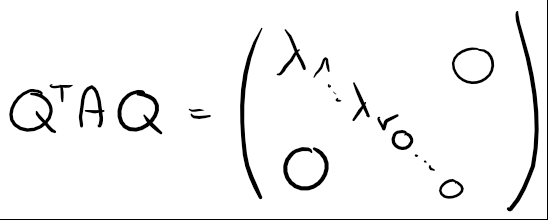
\includegraphics{Ziel_15_1_1.png}
\\
Indem man (falls nötig) die erste Spalte von $Q$ durch ihr Negatives ersetzt, kann man ohne Einschränkung annehmen, dass $Q \in SO(n)$.\\
Sei $y = Q^Tx, \tilde{b} = Q^T b$. Dann führt die Bedingung $x^TAx+b^Tx+c = 0$ zu 
\[
x^T A x + b^T x +c = (Q ^Tx)^T(Q^TAQ)(Q^Tx) +(Q^Tb)^TQ^Tx+c
\]
\[= \lambda_1y_1^2+...+\lambda_ry_r^2 + \tilde{b}_1 y_1 + ... \tilde{b}_n y_n + c = 0\]
Die gemischten quatratischen Terme sind also durch Drehung des Koordinatensystems entfallen.
\item[Schritt 2:] Elimination der ersten $r$ linearen Terme. Sei 
\[\tilde{z}_i = y_i+ \frac{\tilde{b}_i}{2\lambda_i} ,\ i=1,...,r\]
\[\tilde{z}_i = y_i ,\ i=r+11,...,n\]
Dann erhalten wir:
\[
\lambda_1 \tilde{z}_1^2 + ... + \lambda_r \tilde{z}_r^2 + \tilde{b}_{r+1} \tilde{z}_{r+1}+...+ \tilde{b}_n \tilde{z}_n + \tilde{c} = 0 \text{ mit}
\]
\[\tilde{c} = c- \sum^r_{i=1} \frac{\tilde{b}_i^2}{4\lambda_i}\]
\item[Schritt 3:] Elimination der Konstanten: ist mindestens einer der Koeffizienten $\tilde{b}_{r+1},...,\tilde{b}_n \neq 0$, so sei
\[
z = \overline{Q} \tilde{z} + \frac{\tilde{c}}{b'}e_{r+1} \text{ mit}
\]
\[
b' = \sqrt{\sum^n_{i=r+1} \tilde{b}^2_i}
\] 
wobei\\
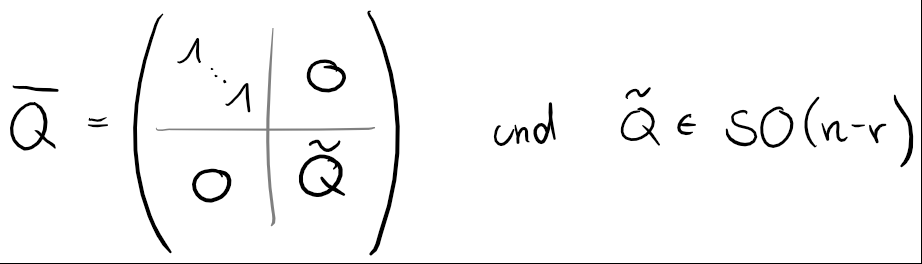
\includegraphics{Ziel_15_1_2.png}\\
mit $\left(
\begin{array}{c}
\tilde{b}_{r+1}\\ \vdots  \\ \vdots\\ \tilde{b}_n
\end{array}
\right) \mapsto \left(
\begin{array}{c}
1\\0\\ \vdots \\0
\end{array}
\right) *b'$\\
Dann:
\[\sum^n_{i=r+1} \tilde{b}_i \tilde{z}_i = 
\left(
\begin{array}{c}
0\\ \vdots \\0 \\ \tilde{b}_{r+1} \\ \vdots \\ \tilde{b}_n
\end{array}
\right)^T \tilde{z}
\]
\[
= \left(
\begin{array}{c}
0\\ \vdots \\0 \\ \tilde{b}_{r+1} \\ \vdots \\ \tilde{b}^n
\end{array}
\right)^T \overline{Q}^T\left(z-\frac{\tilde{c}}{b'} e_{r+1}\right)
\]
\[
= b' e_{r+1}^T \left(z- \frac{\tilde{c}}{b'}\ e_{r+1}\right) = b' z_{r+1} - \tilde{c}
\]
Also:
\[
\lambda_1 z_1^2 +...+ \lambda_r z_r^2 + b' z_{r+1} = 0
\]
\end{description} 
Wir haben also gezeigt:
\section{Satz}
Sei $q(x) = x^TAx + b^Tx +c$ ein quadratisches Polynom im $\mathbb{R}^n$. Dann existiert $Q \in SO(n),\ t\in \mathbb{R}^n$ mit:
\[
q(x) = 0 \Leftrightarrow \tilde{q}(Qx + t) = 0
\]
wobei $\tilde{q}$ eine der folgeden Formen hat:
\[
\tilde{q}(x) = \lambda_1 x_1^2 + ... + \lambda_r x_r^2
\]
\[
\tilde{q}(x) = \lambda_1 x_1^2 + ... + \lambda_r x_r^2-1
\]
\[
\tilde{q}(x) = \lambda_1 x_1^2 + ... + \lambda_r x_r^2-x_{r+1}
\]
und $r = Rang(A)$. Hierbei sind $\lambda_1,...,\lambda_n \in \mathbb{R} \backslash \{0\}$.\\
Die Quadriken der Form $\{x \in \mathbb{R}^n|\tilde{q}(x)=0\}$ werden \textbf{Normalformen} genannt.
\subsection*{Quadriken im $\mathbb{R}^2$ (Kegelschnitte)}
Wir bestimmen die Normalformen von Quadriken im $\mathbb{R}^2$.
\\
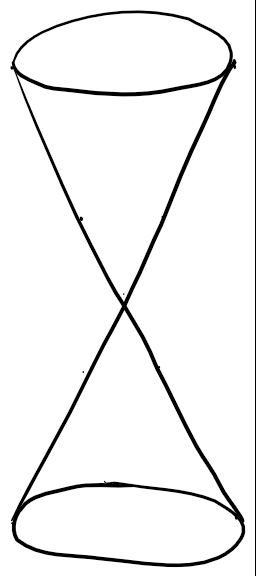
\includegraphics{kegel.png}
\\
\begin{description}
\item[i)] $Rang(A) = 2$
\begin{description}
\item[a)] $\frac{x^2}{a^2} + \frac{y^2}{b^2} -1 = 0 \ (a,b\neq 0)$
\\
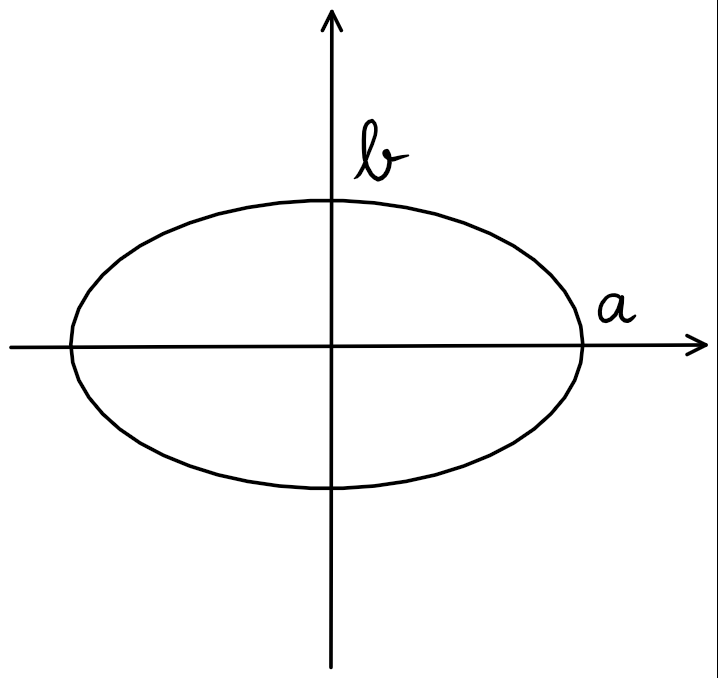
\includegraphics{Satz_15_2_1.png}
\\
Ellipse mit Halbachsen $a$ und $b$.
\item[b)] $\frac{x^2}{a^2} - \frac{y^2}{b^2} -1 = 0$: Hyperbel
\\
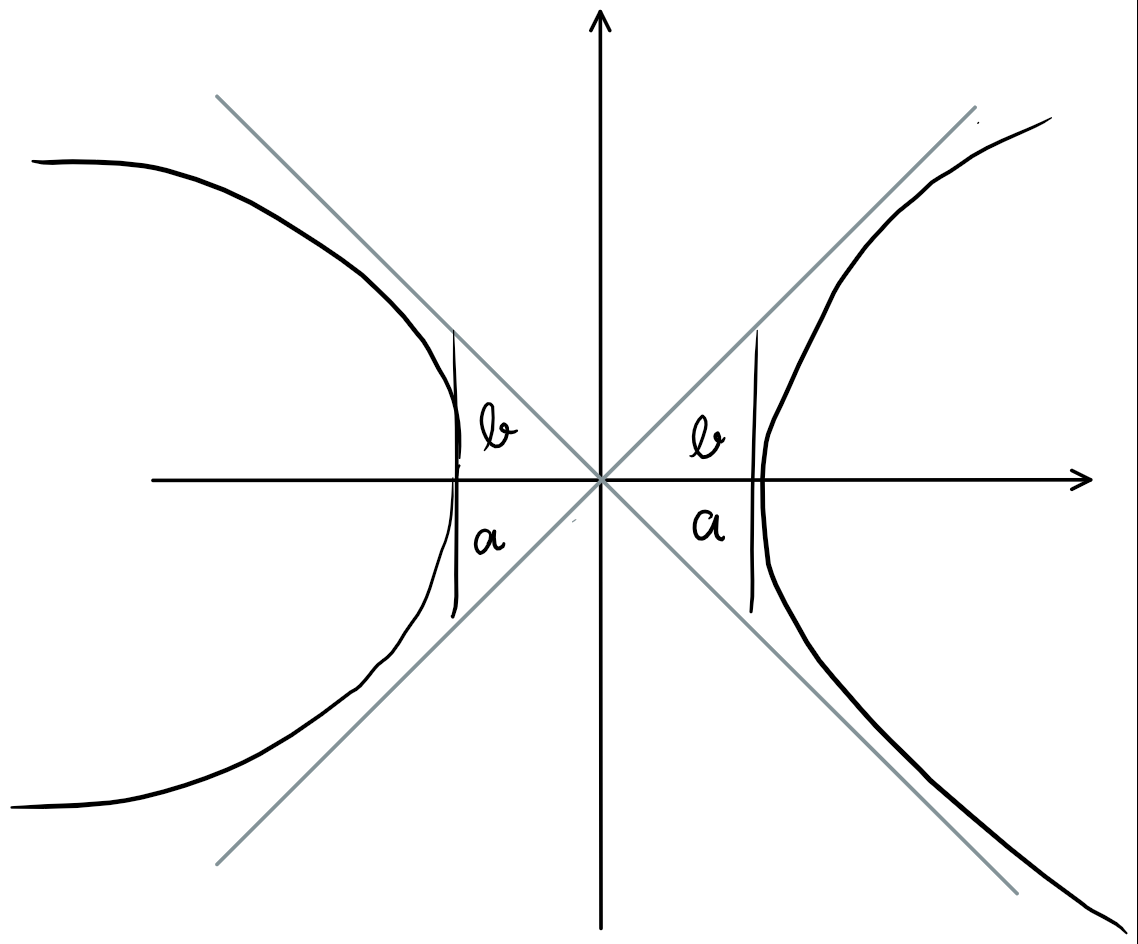
\includegraphics{Satz_15_2_2.png}
\\
\item[c)] $-\frac{x^2}{a^2} - \frac{y^2}{b^2} -1 = 0$: leere Menge
\item[d)] $x^2+ay^2 = 0, \ a\neq 0$: $\left\{ \left(
\begin{array}{c}
0\\0
\end{array}
\right)\right\}$
\item[e)] $x^2-a^2y^2=0,\ a\neq 0$: Geradenpaar
\\
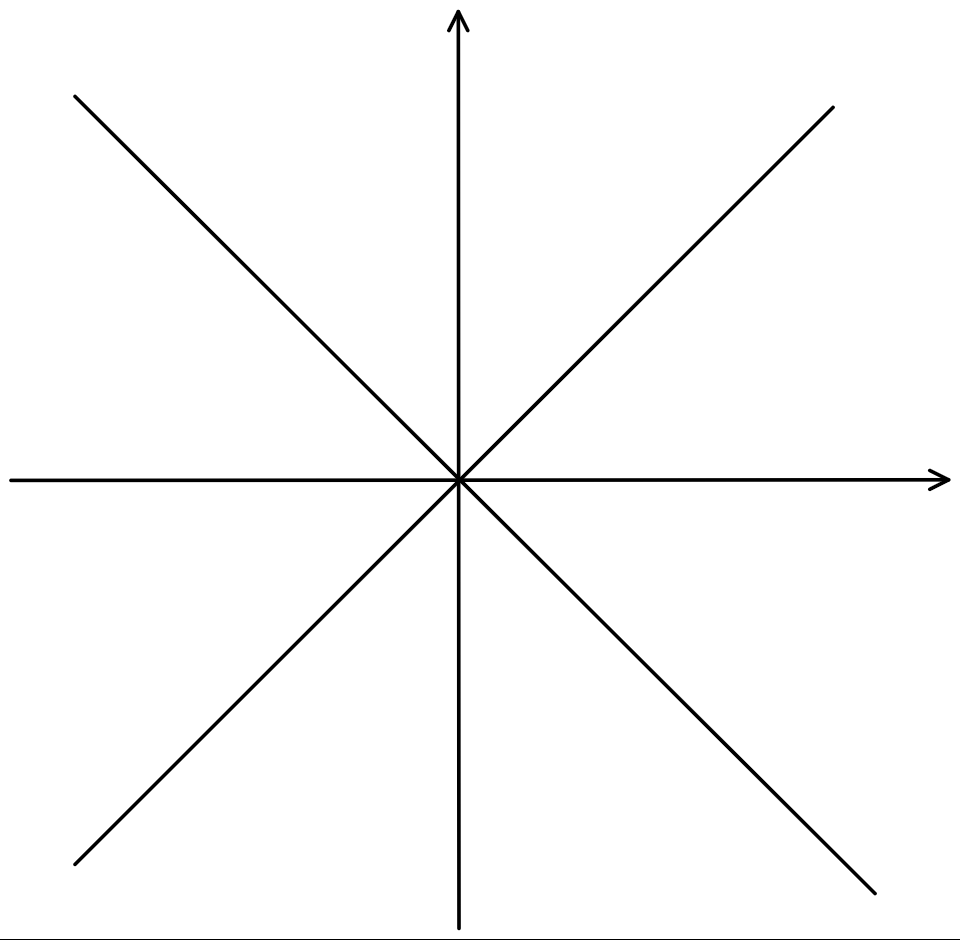
\includegraphics{Satz_15_2_3.png}
\\
\end{description}
\item[ii)] $Rang(A) = 1$
\begin{description}
\item[a)] $x^2-2py = 0 \ (p\neq 0)$: Parabel
\\
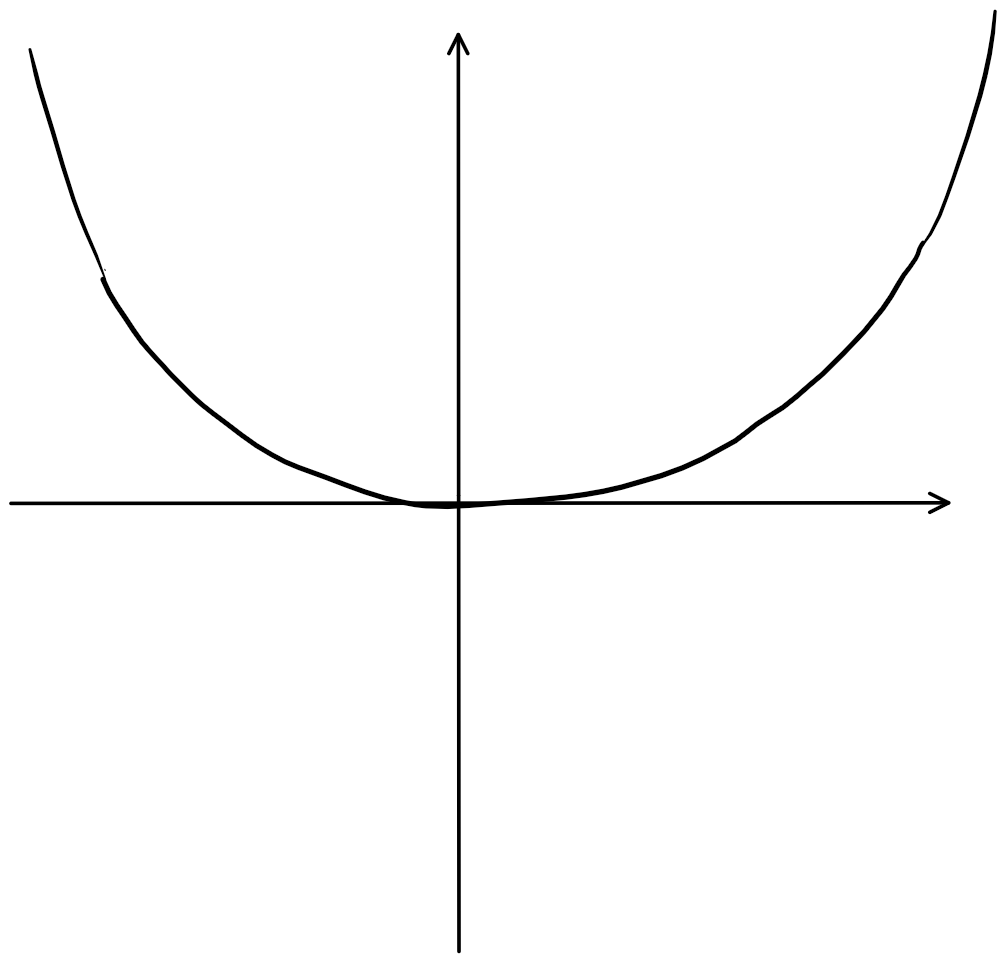
\includegraphics{Satz_15_2_4.png}\[p>0\]
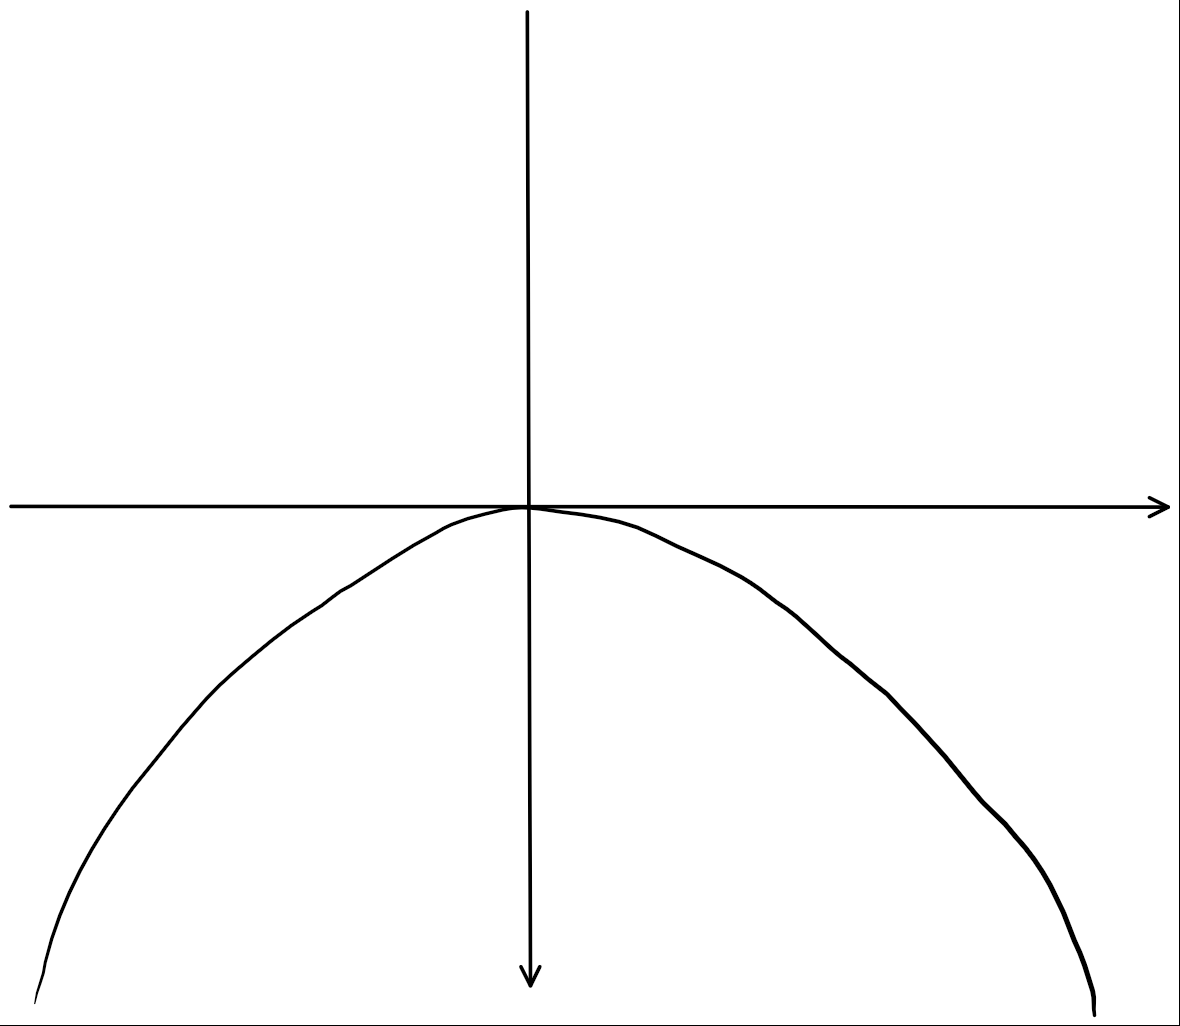
\includegraphics{Satz_15_2_5.png}\[p<0\]

\item[b)] $x^2 -a^2 = 0 \ (a\neq 0)$: zwei parallele Geraden
\\
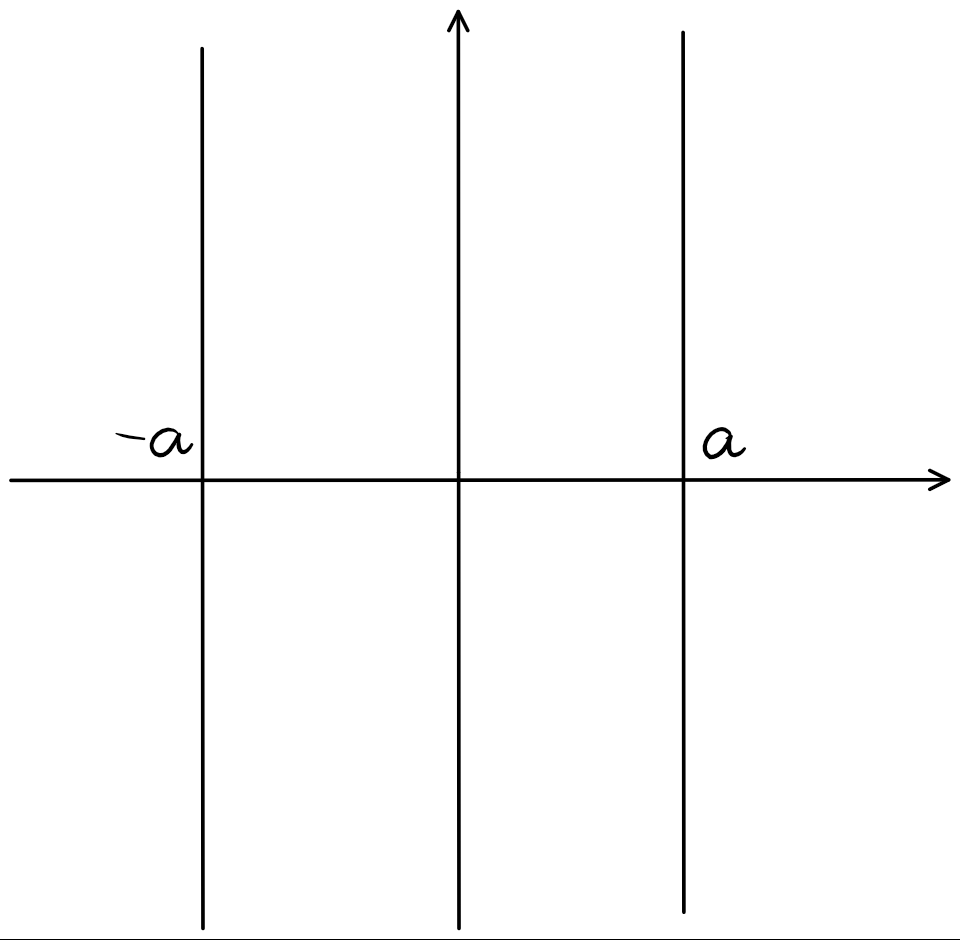
\includegraphics{Satz_15_2_6.png}
\\
\item[c)] $x^2 + a^2 = 0\ (a\neq 0)$: leere Menge
\item[d)] $x^2 = 0$: y-Achse
\end{description}
\end{description}
Quadriken im $\mathbb{R}^3$ siehe Skript Weikert\\
\section{Beispiel}
Gegeben ist das quadratische Polynom
\[q(x)=5x_1^2-4x_1x_2+8x_2^2+ \frac{20}{\sqrt{5}}x_1 - \frac{80}{\sqrt{5}}x_2+4\]
Die zugehörige Quadrik soll auf Normalform gebracht werden. Es gilt:
\[q(x) = x^TAx+b^Tx+c\] mit \[
A=\left(
\begin{array}{cc}
5&-2\\
-2&8
\end{array}
\right), \ b= \frac{1}{\sqrt{5}}\left(
\begin{array}{c}
20 \\-80
\end{array}
\right), c=4
\]
\begin{description}
\item[Schritt 1:] Diagonalisieren von $A$:
\[
\left(
\begin{array}{cc|c}
5-\lambda & -2&0\\
-2&8-\lambda&0
\end{array}
\right)\rightsquigarrow
\left(
\begin{array}{cc|c}
-2&8-\lambda&0\\
5-\lambda & -2&0\\
\end{array}
\right)\rightsquigarrow
\left(
\begin{array}{cc|c}
-2&8-\lambda&0\\
0 & \frac{(5-\lambda)(8-\lambda)-4}{2}&0\\
\end{array}
\right)
\]
Also sind $\lambda_1=9$ und $\lambda_2 = 4$ Eigenwerte von $A$ mit zugehörigen Eigenvektoren (auf Länge 1 normiert):
\[v_1= \frac{1}{\sqrt{5}} \left(
\begin{array}{c}
-1\\2
\end{array}
\right)
,\ 
v_2= \frac{1}{\sqrt{5}} \left(
\begin{array}{c}
-2\\-1
\end{array}
\right)\]
Also folgt mit $Q = \frac{1}{\sqrt{5}}
\left(
\begin{array}{cc}
-1&-2\\
2&-1
\end{array}
\right)$ (so dass also $det(Q)v=1$),\[y=Q^Tx, \ \tilde{b} = Q^Tb =\left(
\begin{array}{c}
-36\\8
\end{array}
\right):\]
\[
9y_1^2+4y_2^2-36y_1+8y_2+4=0
\]
\item[Schritt 2:] Entfernen der linearen Terme durch quadratische Ergänzung:\\
Setze: $z_1=y_1-2, \ z_2=y_2+1$\\
Dann:
\[9z_1^2+4z_2^2-36-4+4=0\]
Also:
\[
\frac{z_1^2}{4} + \frac{z_2^2}{9} = 1
\]
Es liegt alse eine Ellipse mit Halbachsen 2 und 3 vor.
\end{description}
\chapter{Matrixnormen und iterative Verfahren für lineare Gleichungssysteme}
In diesem Abschnitt sei der $\mathbb{R}^n$ versehen mit einer Norm, etwa
\[\|x\|_2 = \sqrt{\sum^n_{i=1}x_i^2}\ \text{"`Euklidsche Norm"'}\]
\[\|x\|_1= \sum^n_{i=1} |x_i| \ \text{"`1-Norm"'} \]
\[\|x\|_\infty= max_{i=1,...,n} |x_i| \ \text{"`Maximumsnorm"'} \]
\section{Definition}
Eine Abbildung $\|\cdot\|_M: \mathbb{R}^{n \times n}\to\mathbb{R}$ heißt \textbf{Matrixnorm}, falls $\|\cdot\|_M$ eine Norm im Sinn von Definition 10.7 ist und zusätzlich
\[
\|A*B\|_M \leq \|A\|_M\|B\|_M \ \forall A,B \in \mathbb{R}^{n\times n} \ \text{(\textbf{Submultiplikativität})}
\]
Eine Matrixnorm $\|\cdot\|_M$ ist \textbf{kompatibel} zu einer Norm $\|\cdot\|_V$ auf dem $\mathbb{R}^n$, falls für $A \in \mathbb{R}^{n \times n}$ und $x \in \mathbb{R}^n$ gilt:
\[
\|Ax\|_V \leq \|A\|_M \|x\|_V
\]
\section{Satz}
Sei $\| \cdot \| _V$ eine Norm auf $\mathbb{R}^n$. Dann definiert
\[
\|A\| := \sup\{
\|Ax\|_V|x \text{ mit } \|x\|_V = 1
\}
\]
eine zu $\| \cdot \|_V$ kompatible Matrixnorm. Sie heißt die $\|\cdot\|_v$ \textbf{zugeordnete Matrixnorm}.
\subsection*{Beweis}
$\| \cdot \|$ ist eine Norm auf $\mathbb{R}^{n \times n}$. Denn:
\begin{description}
\item[(N1)] $\| \lambda A\| = \sup_{\|x\|_V =1} \|\lambda A x\|_V = \sup_{\|x\|_V =1} |\lambda| \|Ax\|_V = |\lambda| \|A\|$
\item[(N2)] $\|A+B\| = \sup_{\|x\|_V =1} \|Ax+Bx\|_V \leq \sup_{\|x\|_V =1}(\|Ax\|_V+\|Bx\|_V)\\ \leq \sup_{\|x\|_V =1} \|Ax\|_V + \sup_{\|y\|_V =1} \|By\|_V = \|A\|+\|B\|$
\item[(N3)]$\|A\| = \sup_{\|x\|_V =1} \|Ax\|_V \geq 0$\\
Ist $\|A\| = 0$, so gilt für alle $x \in \mathbb{R}^n\backslash \{0\}$:
\[\|Ax\|_V = \|x\|_V \|A \frac{x}{\|x\|_V}\|_V \leq \|x\|_V \|A\| = 0\]
Also $Ax=0$ für alle $x \in \mathbb{R}^n$ und somit $A=0$.\\Die in (N3) gezeigte Ungleichung ist gerade die Kompatibilität.\\
Die Submultiplikativität folgt aus:
\[\|AB\| = \sup_{\|x\|=1}\|A(Bx)\|_V 
\underbrace{\leq}_{\text{kompatibilität}}
\sup_{\|x\|_V =1} \|A\|\|Bx\|_V = \|A\|\|B\|
_\square \]
\end{description}
\section{Beispiel}
\begin{description}
\item[i)]Sei $A \in \mathbb{R}^{n \times n},\ \lambda_1$ der größte Eigenwert von $A^TA$ und $B \in O(n)$ mit
\[
B^TA^TAB=\left(
\begin{array}{ccc}
\lambda_1&&0\\
&\ddots\\
0&&\lambda_n
\end{array}
\right)
\]
Dann gilt für alle $x \in \mathbb{R}^n$ mit $\|x\|_2 =1$.
\[
\|Ax\|_2^2 = x^TA^TAx = (B^Tx)^T\left(
\begin{array}{ccc}
\lambda_1&&0\\
&\ddots\\
0&&\lambda_n
\end{array}
\right)B^Tx
\]
\[\leq \lambda_1 \|B^Tx\|^2_2=\lambda_1\]
Gleichheit tritt ein für $x = Be_1$\\
Also:
\[
\|A\|_2 = \sigma_1(A),
\]
wobei $\sigma_1(A)$ der größte Singulärwert von $A$ ist, ist die der Euklidischen Norm zugeordnete Matrixorm. Sie wird \textbf{Spektralnorm} genannt.\\
Sei $A \in GL(n),\ b,\ \tilde{b} \in \mathbb{R}^n,\ x=A^{-1}b, \ \tilde{x} = A^{-1}\tilde{b}$. Dann:
\[
\|x-\tilde{x}\|_2\leq\sigma_1(A^{-1})\|b-\tilde{b}\|_2
\]
\[
\|b\|_2 \leq \sigma_1(A) \|x\|_2
\]
Also:
\[
\|x-\tilde{x}\|_2 \leq \sigma_1(A^{-1}\sigma_1(A) \frac{\|x\|_2}{\|b\|_2}\|b-\tilde{b}\|_2
\]
Aber:
\[
\sigma_1(A^{-1})\sigma_1(A) = \kappa(A) = \frac{\sigma_1(A)}{\sigma_n(A)}
\]
Denn:
\[
\left(
\begin{array}{ccc}
\lambda^{-1}_1&&0\\
&\ddots\\
0&&\lambda^{-1}_n
\end{array}
\right) = (B^TA^TAB)^{-1} = B^TA^{-1}(A^{-1})^TB
\]
Also:
\[\sigma_1(A^{-1})\underbrace{ =}_{\text{Bemerkung 14.3}} \sigma_1((A^{-1})^T)=\sigma_n(A)
\]
Dies zeigt die Stabilitätsabschätzug aus Bemerkung 14.5.
\item[ii)] Sei $x \in \mathbb{R}^n$ mit $\|x\|_1=1$. Dann gilt mit $a_{\cdot j}:=Ae_j$:
\[
\|Ax\|_1 = \|\sum^n_{j=1}x_ja_{\cdot j}\|_1\leq \sum^n_{j=1}|x_j| \|a_{\cdot j}\|_1
\]
\[
\leq max_{j=1,...,n} \|a_{\cdot j}\|_1\underbrace{(\sum^n_{k=1}|x_k|)}_{=1}
\]
\[
= max_{j=1,...,n} \sum^n_{i=1}|a_{ij}|
\]
Ist $j_0$ ein Index, an dem das Maximum angenommen wird, so gilt:
\[
\|Ae_{j_0}\|_1 = \|a_{\cdot j_0}\|_1 = \sum^n_{i=1}|a_{i j_0}|
\]
Also:
\[
\|A\|_1 = max_{j=1,...,n} \sum^n_{i=1}|a_{ij}|\text{ \textbf{Spaltensummennorm}}
\]
ist die der 1-Norm zugeordnete Matrixnorm.
\item[iii)] Sei $x \in \mathbb{R}^n$ mit $\|x\|_\infty =1$. Dann:
\[
\|Ax\|_\infty = max_{i=1,...,n} |\sum^n_{j=1}a_{ij}x_j|
\]
\[max_{i=1,...,n}sum^n_{j=1}|a_{ij}||x_j|\]
\[
\leq \underbrace{max_{k=1,...,n}|x_k|}_{=1} max_{i=1,...,n} \sum^n_{j=1}|a_{ij}| \ (*)
\]
Sei $i_0$ ein Index, an dem das Maximum angenommen wird. Sei $x = \left(
\begin{array}{c}
x_!\\\vdots\\x_n
\end{array}
\right)$ mit $x_j = \left\{
\begin{array}{l}
1,\ a_{i_0j} \geq 0\\
-1,\ a_{i_0j} < 0
\end{array}
\right.$\\
Dann:
\[
\|Ax\|_\infty =\text{max}_{i=1,...,n} \left| \sum^n_{j=1} a_{ij} x_j\right|
\]
\[\leq\text{max}_{i=1,...,n}  \sum^n_{j=1} \left| a_{ij} \right|\left|x_j\right|\]
\[\leq\underbrace{\text{max}_{k=1,...,n} \left|x_k\right|}_{=1} \text{max}_{i=1,...,n} \sum^n_{j=1} \left| a_{ij} \right|\]
Sei $i_0$ ein index, an dem das Maximum angenommen wird.\\
Sei $x = \left(
\begin{array}{c}
x_1\\\vdots\\x_n
\end{array}
\right)$ mit $x_j = \left\{
\begin{array}{ll}
1&,\ a_{i_0j} \geq 0\\
-1&,\ a_{i_0j} < 0
\end{array}
\right.$.\\
Dann:
\[|Ax\|_\infty \geq \left| \sum^n_{j=1}a_{i_0j}x_j\right|=\left| \sum^n_{j=1}a_{i_0j}\right|\geq |Ax\|_\infty\]
Also:
\[|Ax\|_\infty = \text{max}_{i=1,...,n} \sum^n_{j=1} \left| a_{ij} \right| \text{ (\textbf{Zeilensummennorm})}\]
ist die der Maximumsnorm zugeordnete Matrixnorm.
\end{description}
Mit den selben Argumenten wie in Satz 8.4 ii) zeigt man folgende Eigenwertabschätzung;
\section{Satz}
Sei $A\in \mathbb{R}^{n\times n}$, $\lambda$ ein Eigenwert zu $A$ und $\|\cdot\|_M$ eine zu irgend einer Vektornorm $\|\cdot\|_V$ auf $\mathbb{R}^n$ kompatible Matrixnorm. Dann:
\[|\lambda| \leq \|A\|_M\]
\subsection*{Problemstellung:} Sei $A \in \mathbb{R}^{n\times n}$ invertierbar und $b \in \mathbb{R}^n$. Das lineare Gleichungssystem $Ax=b$ soll numerisch gelöst werden.\\
Dazu sei $B$ eine weitere invertierbare $n \times n$-Matrix. Dann:
\[
Bx+(A-B)x =b
\]
Gegeben ein Starvektor $x^{(0)} \in \mathbb{R}^n$ definieren wir $x^(k), k\in \mathbb{N}$, durch:
\[
Bx^{(k)} +(A-B)x^{(k-1)}=b \text{, also}
\]
\[
x^{(k)} = B^{-1}(b-(A-B)x^{(k-1)})=(E_n-B^{-1}A)x^{(k-1)}+B^{-1}b
\]
\section{Satz}
Sei $\|\cdot\|_V$ eine Norm aus $\mathbb{R}^n$ und $\|\cdot\|_M$ eine dazu kompatible Matrixnorm. Dann gilt für alle $k \in \mathbb{N}$:
\[
\|x-x^{(k)}\|_V \leq \|E_n-B^{-1}A\|^k_M\|x-x^{(0)}\|_V
\]
Insbesondere gilt:
\[
\lim_{k\to \infty} \|x-x^{(k)}\|_V = 0,
\]
falls:
\[
\|E_n-B^{-1}A\|_M<1
\]
\subsection*{Beweis}
Da
\[(E_n-B^{-1}A)x+B^{-1}b=x,\]
folgt
\[
\|x-x^{(k)}\|_V = \|(E_n-B^{-1}A)(x-x^{(k-1)})\|_V\]
\[\|E_n-B^{-1}A\|_M\|x-x^{(k-1)}\|_V\]
Die behauptete Ungleichung folgt nun über Induktion über k. $_\square$
\subsection*{Frage}
Wie wählt man B?
\begin{itemize}
\item B sollte einfach zu invertieren sein (Diagonalform oder Dreiecksform)
\item B sollte "`möglichst nahe"' bei A sein.
\end{itemize}
\begin{description}
\item[a)] \textbf{Gesamtschrittverfahren (Jacobi-verfahren)}\\
Hier wählt man für $A = (a_{ij})_{i,j = 1,...,n}$ mit $|a_{ii}| > 0$ für alle $i=1,...,n$:
\[B=
\left(
\begin{array}{ccc}
a_{11}&&0\\
&\ddots\\
0&&a_{nn}
\end{array}
\right)
\]
Dann ist B invertierbar und die iteration
\[Bx^{(k)}+(A-B)x^{(k-1)} = b\]
lautet dann:
\[
a_{ii} x^{(k)}_i + \sum^n_{j=1\ j \neq i}a_{ij} x_j^{(k-1)}=b_i, \ i=1,...,n,\ k \in \mathbb{N}
\]
mit Startvektor $x^{(0)} \in \mathbb{R}^n$
\end{description}
\section{Definition}
Eine Matrix $A \in \mathbb{R}^{n \times n}$ heißt \textbf{strikt diagonaldominant}, falls für alle $i=1,...,n$
\[|a_{ii}| > \sum^n_{j=1\ j \neq i} |a_{ij}|\]
\section{Satz}
Ist $A \in \mathbb{R}^{n \times n}$ strikt diagonaldominant, so konvergiert das Gesamtschrittverfahren für jeden Startvektor $x^{(0)}$ und
\[
\|x-x^{(k)}\|_{\infty} \leq \left(
\text{max}_{i=1,...,n}\frac{\sum_{j\neq i}|a_{ij}|}{|a_{ii}|}
\right)^k \|x-x^{(0)}\|_{\infty}
\]
\subsection*{Beweis}
Es ist dann:
\[E_n-B^{-1}A = (c_{ij})_{i,j=1,...,n}\]
mit
\[c_{ij}=\left\{
\begin{array}{cc}
0&,\ i=j\\
\frac{-a_{ij}}{a_{ii}}&,\ i\neq j
\end{array}
\right.\]
Also:
\[\|E_n-B^{-1}A\|_{\infty} = \text{max}_{i=1,...,n}\sum^n_{j=1\ j\neq i}\frac{|a_{ij}|}{|a_{ii}|}<1.\]
Die Aussage folgt nun aus Satz 16.5 und Beispiel 16.3(iii). $_\square$
\section{Bemerkung} Ist $A \in \mathbb{R}^{n\times n} $ strikt diagonaldominant, so ist $A$ invertierbar. Denn sei $x \ in \mathbb{R}^n$ mit Ax = 0. Sei $i_0$ so gewählt, dass $|x_{i_0}| \geq |x_i|$ für alle $i = 1,...,n$. Durch Übergang von $x$ zu $-x$ (falls nötig) können wir annehmen, dass $a_{i_0i_0}x_{i_0}\geq 0$. Dann:
\[
0 = \sum^n_{j=1 \ j \neq i_0} |a_{i_0j}||x_j|+|a_{i_0i_0}||x_{i_0}|
\]
\[\geq \underbrace{\left(
|a_{i_0i_0}| -\sum^n_{j=1 \ j \neq i_0} |a_{i_0j}| 
\right)}_{>0} \underbrace{|x_{i_0}|}_{=0}\]
Also: $|x_{i_0}| = 0$ uns somit $x_i = 0$ für alle $i=1,...,n$. Die Invertierbarkeit folgt dann aus Satz 4.13.
\begin{description}
\item[b)] \textbf{Einzelschrittverfahren (Gauß-Seidel-Verfahren)}\\
Sei wieder $A = (a_{ij})_{i,j=1,...,n}$ invertierbar mit $a_{ii} \neq 0 $ für alle $i = 1, ..., n$. Setze
\[B=
\left(
\begin{array}{ccc}
a_{11}&&0\\
\vdots&\ddots\\
a_{n1}&\cdots&a_{nn}
\end{array}
\right)
\]
Dann ist $B$ wieder invertierbar und die Iteration
\[Bx^{(k)} + (A-B)x^{(k-1)} = b\]
wird zu
\[a_{ii}x_i^{(k)}+\sum^{i+1}_{j=1}a_{ij}x_j^{(k)}+\sum^{n}_{j=i+1}a_{ij}x_j^{(k-1)},\ i=1,...,n,\ k \in \mathbb{N}\]
Im Vergleich zum Gesamtschrittverfahren werden nun bei der Berechnung von $x^{(k)}_i$ bereits die zuvor berechneten Einträge von $x^{(k)}$, also $x^{(k)}_j$ für j < i, verwendet. \end{description}
Man kann zeigen:
\section{Satz} Das Einzelschrittverfahren konvergiert mit beliebigen Startwert $x^{(0)} \in \mathbb{R}^n $ gegen die Lösung $x \in \mathbb{R}^n$ zu $Ax=b$, d.h. $\lim_{k \to \infty}\| x^{(k)} - x \|_\infty = 0$, falls
\begin{description}
\item[a)] A strikt diagonaldominant oder
\item[b)] A symmetrisch und positiv definit ist.\\
Dies kann mit mehr Aufwand auf Satz 16.5 zurückgeführt werden, siehe Stoer/Bulrisch, Einführung in die numerische Mathematik II, Satz 8.2.12 und 8.3.7
\item[c)] \textbf{Relaxationsverfahren}\\
Man wählt hier in Abhängigkeit von einem Parameter $\omega > 0$:
\[
B(\omega) =
\left(
\begin{array}{cccc}
\frac{a_{11}}{\omega}&&&0\\
a_{21}&\ddots\\
\vdots&\ddots&\ddots\\
a_{n1}&\cdots&a_{n,n-1}&\frac{a_{nn}}{\omega}
\end{array}
\right)
\]
$B(\omega)$ ist unter der Vorraussetzung $a_{ii} \neq 0$ für alle $i=1,..., n$ wiederinvertierbar und 
\[B(\omega)x^{(k)}+(A-B(\omega))x^{(k-1)} = b\]
wird zu
\[
x^{(k)}_i = x_i^{k-1} + \frac{\omega}{a_{ii}}\left(
-\sum_{j=1}^{i-1}a_{ij}x_j^{(k)}
-a_{ii}x_i^{(k-1)}
-\sum_{j=i+1}^n a_{ij} x_j^{(k-1)}
\right)
\]
Für $\omega=1$ ist das gerade das Einzelschrittverfahren, für $\omega > 1$ spricht man von Überrelaxation, für $\omega < 1$ von Unterrelaxation.\\
Ist $A$ symmetrisch und positiv definit, so konvertiert das Relaxationsverfahren für alle $\omega \in (0,2)$, siehe Stoer/Bulirsch, Satz 8.3.7.
\end{description}
\section{Beispiel}
Sei
\[A= \left(
\begin{array}{cc}
2&-1\\
-1&2
\end{array}
\right)
,\ b = \left(
\begin{array}{c}
3\\4
\end{array}
\right)\]
Die exakte Lösung lautet x = $\left(
\begin{array}{c}
\frac{10}{3}\\\frac{11}{3}
\end{array}
\right)$\\
Mit dem Startvektor $x^{(0)} = \left(
\begin{array}{c}
0\\0
\end{array}
\right)$\\
gilt gerundet auf die dritte Hinterkommastelle
\[\left(
\begin{array}{c}
x_1^{(k)}\\x_2^{(k)}
\end{array}
\right)=\left(
\begin{array}{c}
3,333\\3,666
\end{array}
\right)\]
im Gesamtschritverfahren zuerst nach $k = 12$ Iterationen, im Einzelschrittverfahren nach $k=7$ Iterationen und mit Überrelaxation $(\omega=1,15)$ nach $k=5$ Iterationen.\\
In Satz 16.9 wurde die Maximumsnorm auf $\mathbb{R}^n$ verwendet. Diese kann durch jede andere Norm ersetzt werden:
\section{Satz} Sei $\|\cdot\|_V$ eine Norm auf $\mathbb{R}^n$. Dann existieren Konstanten $a, b > 0$ mit 
\[a\|x\|_V \leq \|x\|_\infty \leq b\|x\|_V\]
für alle $x \in \mathbb{R}^n $ \\
Insbesondere gilt für jede Folge $(x^{(k)})_{k \in \mathbb{N}} im \mathbb{R}^n: $
\[ \lim_{k \to \infty} \|x^{(k)}-x \|_V = 0\]
\[\Leftrightarrow \forall_{i=1,...,n} \lim_{k\to\infty} x^{(k)}_i = x_i\]
\subsection*{Beweis} 
Für alle $x\in \mathbb{R}^n$ gilt:
\[
\|x\|_V =
\|\sum^n_{i=1}x_ie_i\|_V
\leq \sum^n_{i=1} |x_i| \|e_i\|_V
\leq \underbrace{\left(
\sum^n_{i=1}\|e_i\|_V
\right)}_{=: a^{-1}}\|x\|_{\infty}
\]
Wir nehmen an, es existiert keine Konstante $b$ die das Geforderte liefert. Dann existiert zu jedem $k\in \mathbb{N} ein x^{(k)} \in\mathbb{R}^n$ mit $\|x^{(k)}\|_\infty > k\|x^{(k)}\|_V$.\\
Sei $y^{(k)}:=\frac{x^{(k)}}{\|x^{(k)}\|_\infty}$\\
Dann gilt für alle $i=1,...,n$: $\left| y^{(k)}_i\right| \leq 1$.\\
Nach dem Satz von Bulzano/Weierstraß (MfI1) konvergiert $(y_1^{(k)})$ entlang einer Teilfolge. Indem man sukzessive Teilfolgen von Teilfolgen bildet, erhält man schließlich eine Teilfolge $(k_l)$ und $y_1,...,y_n \in \mathbb{R}$ mit:\[\lim_{l\to \infty} y^{(k_l)}_i = y_i\] für alle $i=1,...,n$. Sei
\[
\left(
\begin{array}{c}
y_1\\\vdots\\y_n
\end{array}
\right)\in \mathbb{R}^n.
\]
Dann folgt:
\[
\lim_{l \to \infty} \left\|y^{\left(k_l\right)}-y\right\|_\infty = 0
\]
Ferner gilt
\[1= \lim_{l \to\infty} \left\|y^{\left(k_l\right)}\right\|_\infty
\leq \|y\|_\infty + \left\|y^{\left(k_l\right)}-y\right\|_\infty
= \|y\|_\infty
\]
Also: $y \neq 0 \in \mathbb{R}^n\ (*)$
Aber:
\[\|y\|_V \leq \|y-y^{(k_l)}\|_V+\|y^{(k_l)}\|_V\]
\[<a^{-1}\|y-y^{(k_l)}\|_\infty + \frac{1}{k_l}\]
\[
\rightarrow 0 \ (l \to \infty)
\]
Also: $\|y\|_V = 0$ und somit $y = 0 \in \mathbb{R}^n$ im Widerspruch zu $(*)$. $_\square$\\
Man sagt: Alle Normen im $\mathbb{R}^n$ sind äquivalent.
\end{document}